\documentclass[11pt]{article}

\usepackage[utf8]{inputenc}
\usepackage[spanish, es-tabla]{babel}
\usepackage{float}
\usepackage{xcolor}
\usepackage{verbatim}
\usepackage{mwe}
\usepackage{charter}
\usepackage{afterpage}
\usepackage{amsmath}
\usepackage{appendix}
\usepackage{ragged2e}
\usepackage{array}
\usepackage{etoolbox}
\usepackage{fancyhdr}
\usepackage{booktabs}
\usepackage{arydshln}
\usepackage{enumitem}
\usepackage[bottom=3.5cm,top=2.5cm,left=2.0cm,right=2.0cm]{geometry}
\usepackage{graphicx}
\usepackage{indentfirst}
\usepackage{mathtools}
\usepackage{multirow}
\usepackage{pdfpages}
\usepackage{subfiles}
\usepackage{blindtext}
\usepackage{stfloats}
\usepackage{lipsum} 
\usepackage[none]{hyphenat}
\usepackage{hyperref}
\usepackage[ruled,vlined]{algorithm2e}
\usepackage{multicol}
\usepackage[labelfont=bf]{caption}
\usepackage{lscape}

\renewcommand{\algorithmcfname}{Algoritmo}

\renewcommand{\{}{\left\lbrace}
\renewcommand{\}}{\right\rbrace}
\renewcommand{\familydefault}{\rmdefault}

\newcommand\blankpage{
    \null
    \thispagestyle{empty}
    \addtocounter{page}{0}
    \newpage}

\newcolumntype{L}[1]{>{\raggedright\let\newline\\\arraybackslash\hspace{0pt}}m{#1}}
\newcolumntype{C}[1]{>{\centering\let\newline\\\arraybackslash\hspace{0pt}}m{#1}}
\newcolumntype{R}[1]{>{\raggedleft\let\newline\\\arraybackslash\hspace{0pt}}m{#1}}

    \setlist[itemize,1]{label=$\bullet$}
    \setlist[itemize,2]{label=$\circ$}
    \setlist[itemize,3]{label=$-$}
    \setlist{nosep}

\setlength{\columnsep}{30pt}
\setlength{\parskip}{0.15cm}

\pagestyle{fancy}
\fancyhf{}
      
\fancyfoot{}
\fancyfoot[C]{\thepage} % page
\renewcommand{\headrulewidth}{0mm} % headrule width
\renewcommand{\footrulewidth}{0mm} % footrule width

\makeatletter
\patchcmd{\headrule}{\hrule}{\color{black}\hrule}{}{} % headrule
\patchcmd{\footrule}{\hrule}{\color{black}\hrule}{}{} % footrule
\makeatother

\definecolor{blueM}{cmyk}{1.0,0.49,0.0,0.47}

%%%%%%%%%%%%%%%%%%%%%%%%%%%%%%%%%%%%%%%%%%%%%%%%%%%%%%%%%%%%%%%%%%%%%%%%%%%%%%%%%%%%%%%%%%%%%%%%%%%%%%%%%%%%%%%%%%%%%%%%%%%%%%%%%%%%%%%%%%%%%%%%%%%%%%%%%%%%%%%%%%%%%%%%%%%%%%%%%%%%%%%%%%%%%%%%%%%%%%%%%%%%%%
%%%%%%%%%%%%%%%%%%%%%%%%%%%%%%%%%%%%%%%%%%%%%%%%%%%%%%%%%%%%%%%%%%%%%%%%%%%%%%%%%%%%%%%%%%%%%%%%%%%%%%%
\chead[C]{
      \begin{tabular}{m{2cm}m{12cm}m{2cm}}
      \centering
      
\includegraphics[width=1.5cm]{MarcaUS.png}
      &
      \centering
     \fcolorbox{white}{blueM}{\fbox{\begin{minipage}{10cm}
     \centering
     \textcolor{white}{Aplicaciones de Soft-Computing}
     \end{minipage}}}
     &
     \centering
        
\includegraphics[width=1.8cm]{MarcaETSII2.png}    
     \end{tabular}%
    }
    
\cfoot[C]{
    \raggedright
    \begin{tabular}{m{15cm}m{2cm}}
      \hline
      \noalign{\vskip 2mm}
      \raggedright
       \small \textsc{Evaluación Bloque III: Algoritmos Evolutivos}\\
       Autor: \textit{Ramos González, Víctor}.
     &
     \raggedleft
     \thepage   
     \end{tabular}%
    }
    

    
\begin{document}

\hfill\break

\vspace{0.3cm}

{\Large{\textsc{Evaluación Bloque III: Algoritmos Evolutivos}}}\\

{\Large{\textbf{Parte II: Problemas Multiobjetivo con restricciones}}}


\vspace{0.2cm}

\textsc{\textbf{Ramos González, Víctor}} \textit{\footnotesize (vicramgon@alum.us.es)}\\

\vspace{0.1cm}

\begin{tabular}{>{\small}l}
Fecha de elaboración: \textit{\today}\\
Profesor: \textit{Dr. Francisco V. Fernández Fernández}\\
Asignatura: \textit{Aplicaciones de Soft-Computing.} \\
Departamento: \textit{ Electrónica y Electromagnetismo.} \\
\textit{GII. Tecnologías Informáticas - Universidad de Sevilla.}
\end{tabular}



\vspace{11pt}

\centerline{\rule{0.95\textwidth}{0.4pt}}

\begin{center}
    
    \begin{minipage}{0.9\textwidth}
%        % RESUMEN
%        \noindent \textbf{Resumen:} Este trabajo tiene como objetivo principal la implementación de un algoritmo multiobjetivo  basado en agregación así como la comparación del mismo tomando como referencia algunos de los algoritmos utilizados en las clases prácticas de la asignatura, presentando y explicando de forma detallada el algoritmo implementado, los resultados obtenidos y las métricas evaluadas.\\
%        
%        \vspace{4mm}
%        % PALABRAS CLAVE
%        \noindent \textbf{Palabras clave:} Algoritmos Evolutivos, Optimización multiobjetivo, MOEA/D, Soft Computing.
	\renewcommand{\contentsname}{Contenidos}
	\setcounter{tocdepth}{1}
	\tableofcontents
    
    \end{minipage}
    
\end{center}
\centerline{\rule{0.95\textwidth}{0.4pt}}
\vspace{15pt}

\section{ntroducción}
%\section{Introducción}
\justify

Se considera el problema multi-objetivo (sin pérdida de generalidad) consistente en la minimización de $m$ funciones objetivo: $$minimize \, F(\boldsymbol{x})=(f_1(\boldsymbol{x}), \dots, f_m(\boldsymbol{x}))$$ de manera que el espacio de búsqueda $\boldsymbol{x} \in \Omega$ es acotado y corresponde a $\Omega = X_1 \times \cdots \times X_p$, con $X_i$ el conjunto continuo de valores posibles para la componente $x_i$ acotado superior e inferiormente por $x_{Li}$ y $x_{Ui}$ respectivamente.\\

En los problemas de optimización mutiobjetivo, es frecuente que los objetivos sean contrapuestos, esto es, la mejora en uno de los objetivos implica la desmejora de otro, de forma que no existe un único punto que optimice todos los objetivos, si no que se tiene lo que se conoce como frente, en concreto se habla del frente de Pareto o frente Pareto-óptimo.\\

El frente de Pareto corresponde al conjunto de puntos en el espacio de objetivos, tal que ninguno de ellos es dominado por ningún otro de punto de dicho espacio. Dado que un punto $\boldsymbol{u}$ es dominado por otro $\boldsymbol{v}$ si y sólo si $\forall i \in \{1, \dots, m \}: u_i \geq v_i$ y además $\exists j \in \{1, \dots, m\}: u_j > v_j$, esto es $\boldsymbol{u}$ es mejor que $\boldsymbol{v}$ en al menos un objetivo y no es peor en ninguno de los restantes. De forma que el objetivo corresponde, precisamente, a la obtención de este conjunto de puntos. Notaremos la dominancia Pareto como $v \preceq u$.\\

En el estado del arte, existen multitud de aproximaciones a esta categoría de problemas (\textit{MOP}), en este trabajo, se propone abordarla desde la filosofía de los algoritmos evolutivos basados en agregación (\textit{MOEA/D}), que basan su funcionamiento en la descomposición del problema de optimización multi-objetivo en varios subproblemas con un único objetivo (mono-objetivo), de manera que la función objetivo de cada uno de los subproblemas es definida por agregación ponderada de las funciones del problema multi-objetivo. Dentro de este campo existe una amplia variedad de subfilosofías y mejoras al algoritmo original (entre ellas \textit{MOEA/D-DE} \cite{Li2009} o \textit{MOEA/D-DRA} \cite{Qingfu2009}) pero nosotros nos referiremos generalmente a las mismas como \textit{MOEA/D}.\\

Para generar los distintos problemas mono-objetivo existen distintas formulaciones (como \textit{Weighted Sum} o \textit{Boundary Intersections} \cite{Zhang2008}), en este trabajo se seguirá la formulación más corriente en la literatura dada por Tchebychef como: $$ g^{te}\left(\boldsymbol{x}|\boldsymbol{\lambda},\boldsymbol{z^{*}}\right) = \max \limits_{1 \leq i \leq m} \{\lambda_i \, \left|f_{i}(\boldsymbol{x}) - z_{i}^{*}\right|\}$$ donde $\boldsymbol{\lambda}=(\lambda_i, \dots, \lambda_m)$ corresponde a un vector de pesos y $\boldsymbol{z^{*}}=(z^{*}_i, \dots, z^{*}_m)$ corresponde al vector cuyas componentes corresponden a los valores óptimos (mínimos) de las funciones objetivo consideradas de forma aislada, esto es: $$ z_i^{*} = \min \{ f_{i}(\boldsymbol{x}) \, | \,  \boldsymbol{x} \in \Omega \}$$

De forma que, para cada punto $\boldsymbol{x}^{*}$ del frente de Pareto existe un vector de pesos $(\boldsymbol{\lambda})$ tal que  $\boldsymbol{x}^{*}$ es solución óptima del subproblema asociado a $(\boldsymbol{\lambda})$, de manera que recorriendo completamente los posibles $\boldsymbol{\lambda}$ se obtendrían todos los puntos del frente Pareto-óptimo. Computacionalmente, nos quedaremos con una muestra de todos los posibles vectores de pesos $\boldsymbol{\lambda}$, de forma que tratemos de obtener una aproximación al frente de Pareto completo.\\


La filosofía \textit{MOEA/D} se enmarca dentro de los conocidos como \textit{Algoritmos Evolutivos} y como tal uno de los pasos fundamentales del funcionamiento del mismo se basa en la mutación y recombinación de los individuos de la población. En este aspecto la literatura está plagada de distintos operadores, dentro de los cuales los basados en \textit{Evolución Diferencial} son claramente los más numerosos. En este trabajo compararemos tres operadores (\textit{EOP1}, \textit{EOP2}, \textit{EOP3}), sobre un mismo marco de desarrollo, mostrando tanto la metodología seguida como la implementación realizada y los resultados obtenidos, evaluando, mediante el uso de distintas métricas características en la literatura (\textit{Hypervolume}, \textit{Spacing}, \textit{Cober Set}), la eficacia del algoritmo presentado (y los distintos operadores) en relación a otros presentados en este mismo ámbito (\textit{NSGA-II}).\\

%%%%%%%%%%%%%%%%%%%%%%%%%%%%%%%%%%%%%%%%%%%%%%%%%%%%%%%%%%%%



\section{Metodología}
\subsection{Funcionamiento general del algoritmo}


La \hyperref[fig:1]{\textit{figura 1}} muestra el diagrama de flujo general del algoritmo, ajustándose a un esquema típico de algoritmo evolutivo. De manera superficial, el algoritmo recibe las funciones objetivo, las funciones de restricción, el espacio de búsqueda y una serie de parámetros que intervienen en el algoritmo (detallados más adelante), lleva a cabo una primera etapa de inicialización de la población, los vectores de pesos y vecindad de los subproblemas, así como el punto de referencia y las evaluaciones de la población frente tanto a los objetivos como a las restricciones. A partir de ahí se lleva a cabo un proceso iterativo, en el que se va actualizando la población así como el punto de referencia. De forma que al fin del proceso la población constituye la aproximación del algoritmo al frente de Pareto para el problema tratado, distinguiendose para cada una de ellas las que son factibles (cumplen las restricciones) y las que no.\\


\subsection{Datos de entrada}

El algoritmo recibe como datos de entrada:\\
\begin{itemize}
    \item \textbf{Funciones objetivo}: Un conjunto ordenado de funciones $f_1, \dots, f_m$  consideradas como las funciones objetivo a optimizar por el algoritmo, tratando todas ellas como caso de minimización.\\
    
    \item \textbf{Restricciones}: Un conjunto ordenado de funciones $g_1, \dots, g_n$  consideradas como las restricciones del problema en formato $g_j(\boldsymbol{x})\geq 0$.\\
    
     \item \textbf{El espacio de búsqueda $\Omega$}: Dado por el producto cartesiano de los espacios de búsqueda de cada una de las variables, acotados superior e inferiormente por $x_{Lj}$ y $x_{Uj}$ respectivamente.\\

	\item \textbf{$N$}: Corresponde al número de subproblemas considerados para la división del objetivo mútiple en subobjetivos individuales (por agregación).\\
	
	\item \textbf{$G$}: Corresponde al número de generaciones máximo que realizará el algoritmo, estableciendo un criterio de parada para el mismo.\\
	  
    \item \textbf{$T$}: Corresponde al número de vecinos de cada subproblema esto es, el número de subproblemas, incluyéndose a sí mismo, que serán considerados parte de la vecindad de cada uno de los subproblemas y que influirán en el proceso evolutivo de la población.\\
    
	\item \textbf{Operador evolutivo}: Durante el desarrollo del algoritmo son utilizados operadores de cruce y mutación que han de ser dados por el usuario y que obtendrán un solo individuo como descendiente de cada uno de los individuos de la población. En este trabajo utilizaremos el operador EOP1 presentado en la primera parte (optimización no restringida).\\
    
	\item \textbf{Otros parámetros}, que detallamos y justificamos en el apartado correspondiente.\\
\end{itemize}

\subsection{Inicialización del algoritmo}

Para poder llevar a cabo la ejecución del algoritmo (proceso iterativo) hemos de disponer de algunos elementos que debemos inicializar al comienzo del algoritmo como son: \\

\begin{itemize}
    \item \textbf{El conjunto de vectores de pesos $\boldsymbol{\lambda_1}, \dots, \boldsymbol{\lambda_N}$}, vectores $m$-dimensionales que identifican a cada subproblema, de forma que para todos ellos debe cumplirse $||\boldsymbol{\lambda_{i}}||_{1} = 1$ y además deben estar distribuidos uniformemente (equiespaciados, tomando como distancia la forma euclídea). Para el caso bi-objetivo, dado que los vectores han de estar normalizados, los $N$ vectores pueden inicializarse siguiendo la expresión $\boldsymbol{\lambda_i} = \left(\frac{i-1}{N-1}, \frac{N-i}{N-1} \right)$ con $i \in \{1, \dots, N\}$.\\
    
    \item \textbf{Vecindad $B(i)$ de cada vector peso $\boldsymbol{\lambda_i}$}, que corresponde al conjunto de los  los $T$ vectores más cercanos a $\boldsymbol{\lambda_i}$ de entre todos los vectores de pesos (incluyendo al propio $\boldsymbol{\lambda_i}$). Nótese que $B(i)$ será considerado el entorno del subproblema $i$, de manera que debe considerarse un entorno cercano ($T$ pequeño) para la evolución del individuo asociado al subproblema considerado.\\

    
    \item \textbf{Inicialización de la población $P$}, con $N$ individuos cada uno de ellos asociados a uno de los subproblemas. Para la inicialización se generará una población aleatoria (respetando los espacios de búsqueda para cada variable). \\

    \item \textbf{Inicialización del punto de referencia $\boldsymbol{z}$}. Recuérdese que según la formulación de Tchebycheff $\boldsymbol{z}^{*}$ debe contener los óptimos globales de cada una de las funciones objetivo en el espacio de búsqueda, pero esto implica resolver $m$ problemas de optimización mono-objetivo. En vez de eso relajaremos $\boldsymbol{z^{*}}$ en $\boldsymbol{z}$ de forma que contendrá en cada momento el mejor (menor) valor para cada $f_j$ ($j = 1, \dots, m$) alcanzado por cualquiera de los individuos tanto factibles como infactibles, evaluados hasta ese instante. De forma que dicho punto de referencia $\boldsymbol{z}$ se irá actualizando de forma síncrona al avance del algoritmo.\\
    
    \item \textbf{Inicialización del conjunto de soluciones no dominadas}. Opcionalmente, el algoritmo puede mantener un conjunto con las soluciones no dominadas por ninguna otra encontrada hasta el momento de forma que el conjunto será actualizado a lo largo del proceso evolutivo, realizándose dicha actualización de acuerdo al concepto extendido de Pareto-dominancia.\\
\end{itemize}

\subsection{Desarrollo iterativo}

Tras la inicialización, comienza un proceso iterativo (evolutivo) en el que la población, se actualiza por medio del uso de operadores evolutivos y métodos de manejo de restricciones (métodos de señección) que presentaremos a continuación. Como criterio de parada para este proceso iterativo se tomará el límite de generaciones fijado por el usuario (al igual que en otros algoritmos de carácter evolutivo o inteligencia colectiva se pueden fijar otros criterios de parada anticipada). De manera que para cada iteración (generación) se llevan a cabo las siguientes operaciones:\\

\begin{enumerate}
	\justifying
	
    \item \textit{Reproducción}: Para cada uno de los individuos se aplica el operador evolutivo (cruces y/o mutaciones) de forma que cada individuo es perturbado (en mayor o menor medida) por el entorno. Como entorno se considera el vecindario $B(i)$, del que son tomados, con cierta aleatoriedad, (según el operador) una serie de individuos con los que se aplican los operadores evolutivos. Como el vecindario son los considerados problemas cercanos, es esperable que los cambios entre ellos sean pequeños por lo que los individuos tenderán a ser parecidos.\\
    
    En concreto se utilizará el operador EOP1 derivado de Evolución Diferencial + Perturbación Gaussiana, presentado (implementado y evaluado) en la primera parte del trabajo. de forma que el mismo del siguiente modo:\\

    \begin{enumerate}
        \item  El individuo $\boldsymbol{P_i}$ se genera el vector mutante $\boldsymbol{\hat{y}}$, con el uso de cinco vectores `noisy', mediante la expresión  $$\boldsymbol{\hat{y}}=\boldsymbol{x}^{(r1)} + F \cdot (\boldsymbol{x}^{(r2)}- \boldsymbol{x}^{(r3)}) + rand \cdot  F \cdot (\boldsymbol{x}^{(r4)}- \boldsymbol{x}^{(r5)}) $$ donde $F$ es elegido aleatoriamente de un pool de valores (entre $0$ Y $1$) y $rand$ corresponde a un número aleatorio (entre $0$ y $1$).\\
        
        \item  Tras esto, se realiza una recombinación utilizando el cruce típico de evolución diferencial, tal que cada componente del vector $\boldsymbol{y}$ se elige aleatoriamente entre $\boldsymbol{\hat{y}}$  y $\boldsymbol{P_i}$, de forma que $\boldsymbol{y}$ contenga al menos una componente del vector mutante. Para ello se sigue la expresión: $$ y_j = \left\lbrace \begin{array}{cl}
            \hat{y}_{ij} & \textrm{si } rand \leq \textit{CR} \textrm{ o } j = \delta\\
             P_{ij} & e.o.c.
        \end{array} \right. $$ donde \textit{CR} corresponde a un parámetro ajustable (entre $0$ y $1$) que representa la probabilidad de cruce, $\delta$ corresponde a una de las componentes del descendiente elegida aleatoriamente y $rand$ corresponde a un número aleatorio (entre $0$ y $1$).\\
        
        \item Finalmente cada componente de $\boldsymbol{y}$ es perturbada con probabilidad $p_m$ (parámetro ajustable entre $0$ y $1$, típicamente establecida en la literatura como $1/p$, con $p$ la dimensionalidad del espacio de búsqueda) mediante una distribución gaussiana ($N(0,\sigma_{j} = \frac{x_{Uj} - x_{Lj}}{SIG})$ con $SIG$ un parámetro ajustable).\\
        
        \item Reparación: si alguna de las componentes quedara fuera del espacio de búsqueda según las cotas su valor es establecido al valor de la más cercana.\\
    \end{enumerate}

    \item[2.] \textit{Evaluación}: El descendiente obtenido es evaluado respecto a todos los objetivos $\boldsymbol{F}(\boldsymbol{y})$ y respecto a todas las restricciones definiéndose $V(\boldsymbol{y}) = \left\vert \sum \limits_{j=1}^{n} min(0, g_j(\boldsymbol{y})) \right\vert$ (cuantía da violación de restricciones).\\
    
    \item[3.] \textit{Actualización del punto de referencia $\boldsymbol{z}$}: Recuérdese que $z$ correspondía al vector $m$-dimensional ($m$ el número de objetivos) cuyas componenetes correspondientes correspondían a los pseudo-óptimos (mejores valores obtenidos hasta el momento) luego hemos de actualizar $z$ en aquellas componentes tal que $F_j(\boldsymbol{y}) < z_j$ (con $j=1,\dots,m$). Nótese que el punto de referencia es actualizado de igual forma tanto con soluciones factibles como infactibles.\\
    
    \item[4.] \textit{Actualización del entorno $B(i)$}: El vecindario del subproblema $i$ (en el que se incluye él mismo) es actualizado siguiendo un criterio de selección. En este trabajo vamos a presentar un criterio mixto, basado en el concepto de dominancia pareto (separación de objetivos y restricciones)  (Constraint Goals Separation,\textit{CGS}) y en el concepto de función penalti. Este último suele ser más utilizado en la literatura y existen multitud de versiones \textit{Static}, \textit{Multi-staged}, \textit{Dynamic}, \textit{Self-adaptative}, \textit{Three-steps}, ... \cite{Vaz}. Además las penalizaciones puden ser aplicables en las funciones objetivo o una vez calculada $g^{te}$. En la literatura la tendencia a seguir es esta última dando mejores resultados, por lo que nosotros adoptaremos esta visión. Nuestra perspectivas estudiadas se basan en \cite{Fan2017,Asafuddoula2012,Yang2020,Jan2010,Zhu2019}) en los que se han comprobado la eficiencia y eficacia de métodos de selección adaptativos, con penalización basada en umbralización, remplazo en la élite, etc. En concreto se han implementado dos métodos, uno basado en umbralización y otro basado en penalización adaptativa + \textit{CGS}.\\
    
     En concreto los operadores toman $\boldsymbol{x_j}$ el individuo considerado en la actualización con valoración $\boldsymbol{F}(\boldsymbol{x_j})$ y cuantía de violación de restricciones $V(\boldsymbol{x_j})$ y $\boldsymbol{y})$ el descendiente con valoración $\boldsymbol{F}(\boldsymbol{y})$ y violación de restricciones $V(\boldsymbol{y})$, entonces:\\
    
    \noindent$\boxed{\textsc{Operador 1}}$\\
    \begin{enumerate}
    \item Se calculan $fitness(\boldsymbol{x_j})$ y   $fitness(\boldsymbol{y})$ aplicando:  $$ fitness(\boldsymbol{x}) = g^{te}(\boldsymbol{x} \vert \lambda_j, \boldsymbol{z}^{*}) + \sigma \cdot min(\tau, V(\boldsymbol{x}))^{2} + \eta \cdot (0, V(\boldsymbol{x}) - \tau)$$ donde $\tau = Vmin + 0.3 \cdot (Vmax - Vmin)$ con $Vmax$ y $Vmin$ los valores máximo y mínimo de violación de restricciones en el vecindario del problema $j$; $\sigma$ la penalización por debajo de umbral y $\eta$ la penalización por encima del umbral. Nótese que se pretende realizar la búsqueda por la zona factible y la zona infactible cercana a la factible. Por ello conviene que $\sigma << \eta$, así en la literatura $\sigma=0.01$ y $\eta=20$.\\
          
    \item Si $fitness(\boldsymbol{x_j}) >= fitness(\boldsymbol{y})$ entonces se actualiza el individuo del subproblema $j$ con $\boldsymbol{y}$. \\
    \end{enumerate}
    
    \noindent $\boxed{\textsc{Operador 2}}$\\
    \begin{enumerate}
    \item Si $V(\boldsymbol{y})=0 \wedge \left(V(\boldsymbol{x_j}))>0 \vee g^{te}(\boldsymbol{y}| \lambda_j, \boldsymbol{z}) \leq  g^{te}(\boldsymbol{x_j}| \lambda_j, \boldsymbol{z})\right)$  entonces se actualiza el individuo del subproblema $j$ con $\boldsymbol{y}$ \\
          
    \item Si no $fitness(\boldsymbol{x_j}) >= fitness(\boldsymbol{y})$ entonces se actualiza el individuo del subproblema $j$ con $\boldsymbol{y}$. Donde $fitness$: $$ fitness(\boldsymbol{x}) = g^{te}(\boldsymbol{x} \vert \lambda_j, \boldsymbol{z}^{*}) + \eta \cdot V(\boldsymbol{x}); \quad \eta = 10^{\frac{it}{G}} $$ de forma que el valor de penalización por violación de restricciones se adapta según la iteración, de forma que al principio la penalización es pequeña permitiendo la exploración en beneficio del objetivo, pero al final es más alta guiando a las soluciones hacia la zona factible.\\
    \end{enumerate}
    

      Hemos de notar también que la actualización de los vecinos (con ambos operadores) puede conllevar una gran pérdida de la diversidad mucho más apreciable que en el caso no restringido. Por ello se limita la capacidad de actualización a un número de actualizaciones muy bajo (normalmente menor del 5\% del tamaño de la población).Además dado el proceso iterativo propuesto, aunque no ha sido especificado, el proceso de actualización de la población (y sus valoraciones) se realiza directamente sobre la población, y no se espera para ser efectiva al fin de la generación. Por ello es conveniente que a la hora de llevar a cabo las actualizaciones los elementos se recorran en un orden aleatorio, para tratar de evitar descompensaciones entre los individuos.\\
      
       \item[5.] \textit{Actualización del \textit{NDS}}: El conjunto de soluciones no dominadas es actualizado según el criterio extendido de dominancia Pareto, forma que una solución $s_a$ domina a otra $s_b$ (y se nota por $s_a \succ_{ext} s_b$) en los siguientes casos:\\ 
       \begin{itemize}
       		\item Si $s_a$ es factible ($V_a=0$) y $s_b$ es infactible ($V_b=0$).\\
       		\item Si ambas son factibles y $s_a$ domina a $s_b$ según la Parteto-dominancia (clásica), esto es si $s_b$ no mejora a $s_a$ en ningún objetivo y $s_a$ mejora a $s_b$ en al menos uno de los objetivos.\\
       \end{itemize}\
\end{enumerate}

\subsection{Final del algoritmo}

\justify

El proceso iterativo previo se realiza hasta alcanzar el criterio de parada, dado por el número máximo de generaciones $G$. De forma que al final del proceso en la última población se tienen justamente los mejores individuos encontrados durante el proceso para cada uno de los subproblemas y cuyas valoraciones constituyen, precisamente, la aproximación al frente de Pareto. \\

También es posible, y casi más fiel, considerar el $NSD$ una aproximación más cercana y más amplia al frente real Pareto-óptimo, dado que en él se encontrarán todas aquellas soluciones no dominadas por ninguna otra de las encontradas durante todo el proceso de búsqueda.\\ 




\section{Implementación}
%\section{Implementación}


\justifying
\noindent\begin{minipage}[H]{0.5\linewidth}

En este apartado describiremos la implementación concreta realizada de la metodología previamente propuesta, concretando cada una de las etapas y procesos. En el \hyperref[alg:1]{\textit{algoritmo 1}} se presenta el pseudocódigo del marco general de desarrollo, del algoritmo. En los puntos esta sección concretaremos cada una de las partes del mismo, dando los detalles de implementación correspondientes.\\

\subsection{Datos de entrada}

Como se propone en la metodología los datos de entrada corresponden a:\\

\begin{itemize}
    \item \textbf{Funciones objetivo $f_1, \dots, f_m$}:  Dadas como una lista de longitud $m$ de funciones, que reciban como entrada un indivividuo (vector $p-dimensional$) y devuelvan una valor real correspondiente a la valoración del individuo respecto de dicha función.\\
\end{itemize}

\begin{itemize}
	\item \textbf{Restricciones $g_1, \dots, g_n$}:  Dadas como una lista de longitud $n$ de funciones, que reciban como entrada un indivividuo (vector $p-dimensional$) y devuelvan una valor real correspondiente a la valoración del individuo respecto de dicha función.\\
	
    \item \textbf{El espacio de búsqueda $\Omega$}: Que establece para cada una de las variables los límites de variación (continua) de la variable. De forma que dichos límites se darán como una lista de longitud $p$ de pares ($x_{Lj}, x_{Uj}$) de valores reales. Dichos pares son ordenados para asegurar que $x_{Lj} \leq x_{Uj}$.\\
     
     \item \textbf{Número de subproblemas $N$}: Un entero que corresponde al número de subproblemas considerados, esto es el número de vectores de pesos $\boldsymbol{\lambda_i}$ y el tamaño considerado para la población.\\
     
    
    
\end{itemize} 

\end{minipage} \hfill
\begin{minipage}[H]{0.47\linewidth}
    \begin{algorithm}[H]
\SetAlgoLined
 \textbf{Entrada}:
 \begin{itemize}
 
     \vspace{0.15cm}\item MOP: 
     \begin{itemize}
         \vspace{0.15cm}\item[] $\boldsymbol{F}=[f_1, \dots, f_m]$
         \vspace{0.15cm}\item[] $\boldsymbol{C} =[g_1, \dots, g_n]$
         \vspace{0.15cm}\item[] $\Omega =[(x_{L1}, x_{U1}), \dots, (x_{Lp}, x_{Up})]$
     \end{itemize}
     
    \vspace{0.15cm}\item $N$: número de subproblemas
     
    \vspace{0.15cm}\item $G$: número de generaciones
     
    \vspace{0.15cm}\item $T$: número de vecinos

    \vspace{0.15cm}\item $EOP$: operador evolutivo

    \vspace{0.15cm}\item $UN$: Updations number

    \vspace{0.15cm}\item $NDS$: Usar/no usar NDS.

 \end{itemize}
 
 \vspace{0.3cm}
  
 \textbf{Inicialización}:
    \begin{itemize}
        \vspace{0.15cm}\item $\boldsymbol{\lambda}$. Vectores de pesos $(\lambda_1, \dots, \lambda_N)$
        \vspace{0.15cm}\item $B$. Vecindad de los subproblemas $[[B_{1,1}, \dots, B_{1,T}], \dots, [B_{N,1}, \dots, B_{N,T}] ]$
        \vspace{0.15cm}\item P. Población ($\boldsymbol{I_1}, \dots, \boldsymbol{I_N}$)
        \vspace{0.15cm}\item FP. Valoración de la población ($\boldsymbol{F}(P)$)
        \vspace{0.15cm}\item VP. Violación de restricciones de la población ($\boldsymbol{V}(P)$)
        \vspace{0.15cm}\item $\boldsymbol{z}$. Punto de referencia $(z_1, \dots, z_m)$
        \vspace{0.15cm}\item \textit{Conjunto de soluciones no dominadas (NDS Set)}. 
    \end{itemize}
    
\vspace{0.3cm}
  
 \textbf{Actualización} (hasta el límite $G$):\\
    \textit{Para $i=1, \dots, N$}
        \begin{itemize}
            \vspace{0.15cm}\item $\boldsymbol{y_i} \gets EOP(\boldsymbol{P_i})$
            
            \vspace{0.15cm}\item Evaluar $\boldsymbol{y}$: $\boldsymbol{F}(\boldsymbol{y})$ y $V(\boldsymbol{y})$
            \vspace{0.15cm}\item Actualizar $\boldsymbol{z}$
            \vspace{0.15cm}\item Actualizar soluciones vecinas de $i$.
            \vspace{0.15cm}\item Actualizar NDS Set
        \end{itemize}
    
     
    \vspace{0.3cm} 
    
    \textbf{Salida}:
    \begin{itemize}
        \item Aproximación al frente de Pareto. (NDS Set)
    \end{itemize}
 \caption{Marco gral. del CMOEA/D}
 \label{alg:1}
\end{algorithm}
\end{minipage}\\


\begin{itemize}
 \item \textbf{Número de generaciones $G$}:  Un entero que corresponde al número de máximo de iteraciones llevadas a cabo por el algoritmo.\\
    
    \item \textbf{Número de vecinos $T$}: Un entero correspondiente al número de subproblemas, incluyéndose a sí mismo, que serán considerados parte de la vecindad.\\
\end{itemize}

\subsection{Inicialización}

Durante la fase de inicialización se establecen los valores iniciales para:\\

\begin{itemize}
\item\textbf{ Vectores de pesos $(\boldsymbol{\lambda_1}, \dots, \boldsymbol{\lambda_N})$}, de forma que si el problema es bi-objetivo dichos vectores son generados utilizando la expresión $\boldsymbol{\lambda_i} = \left(\frac{i-1}{N-1}, \frac{N-i}{N-1} \right)$ con $i \in \{1, \dots, N\}$ para $i=1,\dots, N$. Si se desea es posible especificar un fichero en formato \textit{ASCII} del que se leerán las $N$ primeras lineas que deberán contener los vectores de pesos considerados.\\

\end{itemize}


\begin{itemize}

\item \textbf{Vecindad de los subproblemas $B$}. Corresponde a una lista de listas que contienen los índices considerados dentro de la vecindad de un subproblema, de forma que para cada subproblema $i$ son considerados como vecinos los $T$ cuyos vectores asociados son más cercanos a $\boldsymbol{\lambda_i}$. Para ello se crea (temporalmente) un matriz de distancias $D_{N \times N}$ tal que cuya posición $i,j$ corresponde a la distancia euclídea entre $\boldsymbol{\lambda_i}$ y $\boldsymbol{\lambda_j}$. Una vez calculada dicha matriz, el vecindario de $i$ corresponde a los $T$ $j$ con menor $d_{ij}$.\\

\item \textbf{Población $P = [\boldsymbol{I_1}, \dots, \boldsymbol{I_N}]$}. Se inicializa con valores aleatorios (dentro del espacio de búsqueda) para cada una de las variables de cada uno de los individuos. Para ello se genera una matriz $\hat{P}_{N \times p}$ de números aleatorios (entre $0$ y $1$). De forma que ahora $P$ es obtenida aplicando a cada elemento de cada columna la expresión $P_{ij}=\hat{P}_{ij} \left(x_{Uj} - x_{Lj}\right) + x_{Lj}$, obteniendo un número aleatorio entre $x_{Lj}$ y $x_{Uj}$. De forma que la población $P$ es almacenada como una matriz $P_{N \times p}$ en la que cada fila corresponde al individuo $\boldsymbol{P_i}$ asociado al problema $i$; y cada columna corresponde al valor de las características de dicho individuo (genotipo).\\

\item \textbf{Valoración de la población $FP_{N \times m} = \boldsymbol{F}(P)$}. Es inicializada con la valoración de los individuos de $P$. Para ello a cada una de los individuos (filas) de $P$ son valorados según las funciones objetivo $f_1, \dots. f_m$, dando lugar a la matriz $FP$, en la que cada fila $i$ corresponde a las valoraciones del individuo $\boldsymbol{P_i}$ (fenotipo) y cada columna $j$ a la valoración según $f_j$\\ 

\item \textbf{Violación de restricciones de la población $VP^{(N)} = V(P)$}. Es inicializada con la violación de restricciones de cada uno de los individuos de $P$. Para ello a cada una de los individuos (filas) de $P$ se les aplica $V(\boldsymbol{x})= - \sum \limits_{j=1}^{n} \min(g_j(\boldsymbol{x}), 0)$ dando lugar a un vector (o lista) de longitud $N$ con la cuantía de violación (nótese que es positivo, ya que todos los sumandos son no positivos, esto es, negativos o nulos) de cada uno de los individuos.\\ 

\item \textbf{Punto de referencia $\boldsymbol{z} = (z_1, \dots, z_m)$}. Corresponde al vector de los mejores valores encontrados para cada una de las funciones objetivo $f_1, \dots. f_m$. Teniendo en cuenta que inicialmente solo se tienen los individuos de $P$, cuyas valoraciones corresponden a $VP$, para la inicialización de $z$ basta coger el mínimo de cada columna de $FP$ que será el mejor (menor) valor encontrado hasta el momento) indistintamente de si es factible o infactible.\\

\item \textbf{Conjunto de soluciones no dominadas \textit{NDS Set}}. Corresponde al conjunto de vectores en el espacio de objetivos (valoraciones) que no son dominada por ninguna encontrada hasta el momento. Dado que inicialmente solo se han encontrado las soluciones de $VP$ basta recorrer $VP$ y añadir \textit{NDS Set} aquellas que no son dominadas por ninguna otra, utilizando el concepto de Pareto-dominancia extendido. Esto es equivalente a tomar el inicialmente \textit{NDS Set} y realizar una actualización de \textit{NDS Set} con cada solución (vector fila) de $VP$. Dicha actualización se realiza según los pseudocódigos presentados en el \hyperref[alg:2]{algoritmo 2} y el \hyperref[alg:3]{algoritmo 3}\\

\begin{center}
\begin{minipage}[H]{0.45\linewidth}
    \begin{algorithm}[H]
\SetAlgoLined
 \textbf{Entrada}:
 \begin{itemize}
 
     \vspace{0.15cm}\item \textit{NDS}: $(NDS_P, NDS_F, NDS_V)$	
     
    \vspace{0.15cm}\item $\boldsymbol{x}, F^{(x)} = F(\boldsymbol{x}), V^{(x)} = V(\boldsymbol{x})$
 \end{itemize}
 
 \vspace{0.3cm}
  
 \textbf{Actualización del NDS}:\\
        \begin{itemize}
        	\vspace{0.15cm}\item $NDS' \gets copy(NDS)$;
        	\vspace{0.15cm}\item \textit{Para $i=1, \dots, |NDS_P|$}:  \hspace{2.5cm}
        	\begin{itemize}
        		\vspace{0.15cm}\item $F^{(j)} \gets NDS_F[j]$
        		\vspace{0.15cm}\item $V^{(j)} \gets NDS_V[j]$
            	\vspace{0.15cm}\item Si $(F^{(j)},V^{(j)}) \succ (F^{(x)}, V^{(x)})$: STOP
            	\vspace{0.15cm}\item Si $(F^{(x)}, V^{(x)}) \succ (F^{(j)},V^{(j)})$: $NDS'[j] \gets (x, F_x, V_x)$
        	\end{itemize}
        	\vspace{0.15cm}\item Hacer $NDS \gets unique(NDS')$
        \end{itemize}
    \vspace{0.3cm} 
    
    \textbf{Salida}:
    \begin{itemize}
        \item \textit{NDS} Actualizado.
    \end{itemize}
 \caption{Actualización de \textit{NDS}}
 \label{alg:2}
\end{algorithm}
\end{minipage} \;
\begin{minipage}[H]{0.5\linewidth}
    \begin{algorithm}[H]
\SetAlgoLined
 \textbf{Entrada}:
 \begin{itemize}
 
    \vspace{0.15cm}\item $s_a = (F^{(a)}, V^{(a)})$,
     \vspace{0.15cm}\item $s_b = (F^{(b)}, V^{(b)})$
    \vspace{0.15cm}\item $m$: número de objetivos
 \end{itemize}
 
 \vspace{0.3cm}
  
 \textbf{Desarrollo}:\\
        \begin{itemize}
        	\vspace{0.15cm}\item Si $V^{(a)} < V^{(b)}$: devolver \textit{True}
        	\vspace{0.15cm}\item Si $V^{(a)} > V^{(b)}$: devolver \textit{False}
        	\vspace{0.15cm}\item Si $V^{(a)} = V^{(b)}$: 
        	\begin{itemize}
        		\vspace{0.15cm}\item Si $\exists j=1, \dots, m / F_i^{(b)} < F_i^{(a)}$:\\devolver \textit{False} 
            	\vspace{0.15cm}\item Si no, $\exists j=1, \dots, m / F_i^{(a)} < F_i^{(b)}$: devolver \textit{True} 
            	\vspace{0.15cm}\item Si no: devolver \textit{False}
        	\end{itemize}
        \end{itemize}
    \vspace{0.3cm} 
    
    \textbf{Salida}:
    \begin{itemize}
        \item ¿$ s_a \succ_{ext} s_b$? (\textit{True}/\textit{False})
    \end{itemize}
 \caption{Pareto-dominancia ext.}
 \label{alg:3}
\end{algorithm}
\end{minipage}\\
\end{center}

\end{itemize}

\subsection{Desarrollo evolutivo (iterativo)}

Una vez inicializado el algoritmo se lleva a cabo un proceso iterativo de evolución durante $G-1$ iteraciones (de forma que el algoritmo genera en total $G$ generaciones y realiza $G \cdot N$ evaluaciones. Durante cada una de las iteraciones del proceso evolutivo se lleva a cabo:

\subsubsection{Reproducción}

Consistente en la generación de los nuevos descendientes. Para ello, se pueden utilizar distintos operadores evolutivos con la condición de que devuelvan un único descendiente. Para que el algoritmo tenga un carácter más general, se propone que la función generadora de los descendientes $EOP$ sea dada al algoritmo también como entrada, aunque en la experimentación utilizaremos el operador EOP1 descrito a continuación.\\

    \noindent\begin{minipage}{\textwidth}
    
        \begin{algorithm}[H]
    \SetAlgoLined
     \vspace{0.2cm}\textbf{Entrada}:
    \begin{multicols}{2}
     \begin{itemize}
         \vspace{0.15cm}\item $i$: índice del individuo actual 
         \vspace{0.15cm}\item $P$: Población (genotipos)
         \vspace{0.15cm}\item $VP$: Valoración de la población (fenotipos)
         \vspace{0.15cm}\item $B_i$: Índices de vecinos de $i$
         \vspace{0.15cm}\item $\Omega$: Espacio de búsqueda.
         \vspace{0.15cm}\item Parámetros : 
            \begin{itemize}
                \item $Fs$ : Pool de valores para $F$ 
                \item $CR$ : Probabilidad de cruze 
                \item $PM$ : Probabilidad de mutación
                \item $SIG$ : Apertura de la mutación 
            \end{itemize} 
     \end{itemize}
    \end{multicols}
    
    \begin{multicols}{2}
     \vspace{0.2cm} \textbf{(1) Mutación de $\boldsymbol{P_i}$}: Vector mutante $\boldsymbol{\hat{y}}$.
            \begin{enumerate}
                \item $r_1, r_2, r_3, r_4, r_5 \in B_i$.
                \item $\boldsymbol{\hat{y}} \gets \boldsymbol{P_{r1}} + F \cdot (\boldsymbol{P_{r2}} - \boldsymbol{P_{r3}}) + rand \cdot (\boldsymbol{P_{r2}} - \boldsymbol{P_{r3}}) $
            \end{enumerate}
            
     \vspace{0.2cm} \textbf{(2) Cruce de $P_i$ con $\boldsymbol{\hat{y}}$}: 
            \begin{enumerate}
                \item $Cp \gets (\dots,  Cp_\delta=1, \dots) \in \{0,1\}^{p}$.
                \item $y_j \gets Cp \odot \boldsymbol{\hat{y}} +  (\boldsymbol{1}^{(p)} - Cp) \odot \boldsymbol{P_i}
                 $
            \end{enumerate}
            
    \end{multicols}
        
    \begin{multicols}{2}
    \vspace{0.2cm} \textbf{(3) Mutación de $\boldsymbol{y}$}:\\
    Para $j = 1, \dots, dim(\boldsymbol{P_i})$\\
            \begin{enumerate}
                \item Si $rand \in [0,1] < PM $: 
                \begin{enumerate}
                    \item $\sigma_j \gets |x_{Uj} - x_{Lj}|/SIG$
                    \item $y_j \gets y_j + rand \in \mathcal{N}(0, \sigma_j)$ 
                \end{enumerate}
            \end{enumerate}\columnbreak
            
        \vspace{0.2cm} \textbf{(4) Reparación de $\boldsymbol{y}$}: \\
        Para $j = 1, \dots, dim(\boldsymbol{P_i})$\\
            \begin{enumerate}
                \item $y_j \gets \min ( \max ( y_j , x_{Lj}), x_{Uj})$
            \end{enumerate}
    \end{multicols}
       
         \vspace{0.2cm}\textbf{Salida}: Descendiente $y \in \Omega$
     \caption{Pseudocódigo EOP1}
     \label{alg:4}
    \end{algorithm}
     \end{minipage}\\ \vspace{0.2cm}
    
    \noindent\textbf{EOP1}. Basado en DE + GP. En el \hyperref[alg:4]{\textit{algoritmo 4}} se presenta el pseudocódigo de la función que describimos a continuación. El operador evolutivo EOP1 toma un individuo $P_i$ y genera un desciendente $\boldsymbol{y}$ a partir de él, de forma que:\\
    
    \begin{enumerate}
        \item Realiza una primera mutación de $\boldsymbol{P_i}$ (procendente de DE) de forma que se genera un vector mutante a partir de cinco vectores escogidos del entorno de $P_i$. En concreto se escogen al azar cinco elementos del vecindario de $i$ (correspondientes a los subproblemas $r1$, $r2$. $r3$, $r4$ y $r5$, con reemplazamiento si es necesario) y se genera el vector mutante aplicando la expresión descrita a partir de los vectores asociados a los subproblemas que son justamente las filas correspondientes a los índices $r1$, $r2$ y $r3$ de la población (matriz) $P$, de forma que el vector mutante corresponde a $\boldsymbol{\hat{y}} = P_{r1} + F (P_{r2} - P_{r3})$. Con $F$ un parámetro de la función establecido por el usuario (típicamente $0.5$). \\
        
        \item Realiza el cruce del individuo $\boldsymbol{P_i}$ con el vector mutante $\boldsymbol{\hat{y}}$. Para ello se genera un vector de números aleatorios booleanos $\boldsymbol{CP}$ (crossing points) (con probabilidad $CR$, dada por el usuario, típicamente $0.5$), esto es un vector de valores $0$ y $1$, de forma que para garantizar que el vector resultante contiene al menos un elemento del vector mutante, una posición aleatoria de $CP$ es fijada a $1$. Ahora para el vector resultante (descendiente) se toman  de $\boldsymbol{\hat{y}}$ aquellas componentes en las que $CP_j = 1$ y de $\boldsymbol{P_i}$ aquellas que son $0$, esto es justamente (en operaciones vectoriales) $\boldsymbol{y} = \boldsymbol{CP} \odot \boldsymbol{\hat{y}} +  (\boldsymbol{1}^{(p)} - \boldsymbol{CP}) \odot \boldsymbol{P_i}$ (con $\boldsymbol{1}^{(p)}$ el vector $p$-dimensional con todas sus componentes  $1$).\\
        
        \item Realiza una perturbación gaussiana en algunas de las componentes del descendiente. De forma que para cada una de las componentes se sortea aleatoriamente con probabilidad $PM$ (dada por el usuario o en su ausencia $1/p$, con $p$ el número de componentes de los individuos) y en caso favorable dicha componente $y_j$ es perturbada añadiéndole una cantidad aleatoria obtenida de una distribución normal (gaussiana) de media 0 y desviación estándar $\frac{|x_{Uj} - x_{Lj}|}{SIG}$ (donde $SIG$ corresponde a un parámetro ajustable por el usuario, típicamente 20). \\
        
        \item Finalmente cada una de las componentes de $y$ que se encuentren fuera del espacio de búsqueda son ajustadas a la cota correspondiente, equivalente a aplicar la función $y_j = min(max(y_j ,x_{Lj}),$ $x_{Uj})$ sobre cada componente.\\
        
    \end{enumerate}

\subsubsection{Evaluación del descendiente}

Una vez generado el sucesor éste es evaluado respecto a cada uno de los objetivos almacenándose en un vector $\boldsymbol{f_y}$ las valoraciones tal que la posición $k$ de dicho vector corresponde a $f_k(\boldsymbol{y})$.\\

De igual forma el sucesor es evaluado respecto de las restricciones y se calcula $V_y = V(y)$ como la suma de los valores del vector que resulta de dicha evaluación..\\

\subsubsection{Actualización del punto de referencia}

Como $\boldsymbol{z}$ debe mantener en todo momento los mejores valores obtenidos por alguno de los individuos, es necesario actualizar aquellas componentes en las que $\boldsymbol{f_y}$ sea mejor (menor) que $\boldsymbol{z}$, de forma que para cada componente $j=1, \dots, m$, se actualiza $\boldsymbol{z}$ con $z_j = \min(z_j, (f_y)_j)$. \\

\subsubsection{Actualización de los vecinos}

A continuación se aplicará sobre el vecindario el operador de selección,de entre los que han sido presentados en la metodología, cuyos pseudocódigos se presentan en el \hyperref[alg:5]{algoritmo 5} y el \hyperref[alg:6]{algoritmo 6}, siguiendo los pasos descritos detalladamente en la metodología.\\


\subsubsection{Actualización de \textit{NDS Set}}

Para mantener en todo el momento la consistencia del conjunto cada vez que es generado un descendiente se actualiza el conjunto añadiendo la valoración asociada y eliminando las soluciones dominadas por ella, si procede.\\

Para ello se recorre el conjunto de soluciones dominadas, comparando cada solución con $\boldsymbol{F}(\boldsymbol{y})$ en el momento en que se encuentre una que la domine, el proceso es abortado. En caso de que no se encuentre ninguna, se habrán ido eliminando, al mismo tiempo que se recorren, aquellas soluciones dominadas por $\boldsymbol{F}(\boldsymbol{y})$, por lo que basta añadir $\boldsymbol{F}(\boldsymbol{y})$ al conjunto para completar la actualización. \\


\begin{center}
\begin{minipage}[H]{0.8\linewidth}
    \begin{algorithm}[H]
\SetAlgoLined
 \textbf{Entrada}:
 \begin{itemize}
 
     \vspace{0.15cm} \item $i$: el subproblema considerado.
     \vspace{0.15cm} \item $B$: la lista de vecindades. 
     \vspace{0.15cm} \item $P, FP, VP$: la población y su valoración de objetivos y restricciones.
     \vspace{0.15cm} \item $\boldsymbol{\lambda}$: la lista de vectores de pesos.
     \vspace{0.15cm} \item $z$: el vector de mejores valores objetivo.
     \vspace{0.15cm} \item $NDS$: conjunto de soluciones no dominadas.
     \vspace{0.15cm} \item $\boldsymbol{y},\boldsymbol{f_y}, V_y$: el descendiente y su valoración de objetivos y restricciones.
     \vspace{0.15cm} \item $m$: el número de objetivos.
 \end{itemize}
 
 \vspace{0.3cm}
  
 \textbf{Actualización de la vecindad}:\\
        \begin{itemize}
        	\vspace{0.15cm} \item $c=0$,  $\eta= 20$, $\sigma=0.01$;
        	\vspace{0.15cm}\item \textit{Para $j=1, \dots, B(i)$}:
        	\begin{itemize}
        		\vspace{0.15cm}\item $f_x=FP[j]$, $V_x=VP[j]$, 
        		\vspace{0.15cm}\item $Vmin = min\{V_x \in VP[B(j)\}$, $Vmax = max\{V_x \in VP[B(j)\}$, 
        		\vspace{0.15cm}\item $\tau= Vmin + 0.3 \cdot (Vmax - Vmin)$
        		\vspace{0.15cm}\item $fitness_x = max \{\lambda[j][i] \cdot  \left\vert f_x[i]-z[i] \right\vert; i=1, \cdots m\} + \sigma \cdot min(\tau, V_x)^2 + \eta \cdot max(0, V_x-\tau)$
        		\vspace{0.15cm}\item $fitness_y = max \{\lambda[j][i] \cdot  \left\vert f_y[i]-z[i] \right\vert; i=1, \cdots m\} + \sigma \cdot min(\tau, V_y)^2 + \eta \cdot max(0, V_y-\tau)$
        		\vspace{0.15cm}\item Si $fitness_y \leq fitness_x$:
            	\begin{itemize}
            		\vspace{0.15cm}\item $P[j]=\boldsymbol{y}$, $FP[j]=\boldsymbol{f_y}$, $VP[j]=V_y$
            		\vspace{0.15cm}\item $c \gets c + 1$
				\end{itemize}            	 
            	\vspace{0.15cm}\item Si $c \geq UN$: \textit{next} $j$
        	\end{itemize}
        \end{itemize}
    \vspace{0.3cm} 
    
    \textbf{Salida}:
    \begin{itemize}
        \item Población actualizada.
    \end{itemize}
 \caption{Actualización de la vecindad del subproblema $i$ (OS 1)}
 \label{alg:5}
\end{algorithm}
\end{minipage} \\
\end{center}

\begin{center}
\begin{minipage}[H]{0.8\linewidth}
    \begin{algorithm}[H]
\SetAlgoLined
 \textbf{Entrada}:
 \begin{itemize}
 
     \vspace{0.15cm} \item $i$: el subproblema considerado.
     \vspace{0.15cm} \item $B$: la lista de vecindades. 
     \vspace{0.15cm} \item $P, FP, VP$: la población y su valoración de objetivos y restricciones.
     \vspace{0.15cm} \item $\boldsymbol{\lambda}$: la lista de vectores de pesos.
     \vspace{0.15cm} \item $z$: el vector de mejores valores objetivo.
     \vspace{0.15cm} \item $NDS$: conjunto de soluciones no dominadas.
     \vspace{0.15cm} \item $\boldsymbol{y},\boldsymbol{f_y}, V_y$: el descendiente y su valoración de objetivos y restricciones.
     \vspace{0.15cm} \item $it$: el número de generación actual.
     \vspace{0.15cm} \item $G$: el número máximo de generaciones.
     \vspace{0.15cm} \item $m$: el número de objetivos.
 \end{itemize}
 
 \vspace{0.3cm}
  
 \textbf{Actualización de la vecindad}:\\
        \begin{itemize}
        	\vspace{0.15cm} \item $c=0$,  $\eta= 10^{\frac{it}{G}}$;
        	\vspace{0.15cm}\item \textit{Para $j=1, \dots, B(i)$}:
        	\begin{itemize}
        		\vspace{0.15cm}\item $f_x=FP[j]$, $V_x=VP[j]$, 
        		\vspace{0.15cm}\item $gte_x = max \{\lambda[j][i] \cdot  \left\vert f_x[i]-z[i] \right\vert; i=1, \cdots m\}$
        		\vspace{0.15cm}\item $gte_y = max \{\lambda[j][i] \cdot  \left\vert f_y[i]-z[i] \right\vert; i=1, \cdots m\}$
        		\vspace{0.15cm}\item Si $V_y=0 \wedge (V_x>0 \vee gte_x >= gte_y)$:
            	\begin{itemize}
            		\vspace{0.15cm}\item $P[j]=\boldsymbol{y}$, $FP[j]=\boldsymbol{f_y}$, $VP[j]=V_y$
            		\vspace{0.15cm}\item $c \gets c + 1$
				\end{itemize}   
				
				\vspace{0.15cm}\item Si no si $gte_x + \eta \cdot V_x >= gte_y + \eta \cdot V_y)$:
            	\begin{itemize}
            		\vspace{0.15cm}\item $P[j]=\boldsymbol{y}$, $FP[j]=\boldsymbol{f_y}$, $VP[j]=V_y$
            		\vspace{0.15cm}\item $c \gets c + 1$
				\end{itemize}  
				         	 
            	\vspace{0.15cm}\item Si $c \geq UN$: \textit{next} $j$
        	\end{itemize}
        \end{itemize}
    \vspace{0.3cm} 
    
    \textbf{Salida}:
    \begin{itemize}
        \item Población actualizada.
    \end{itemize}
 \caption{Actualización de la vecindad del subproblema $i$ (OS 1)}
 \label{alg:5}
\end{algorithm}
\end{minipage} \\
\end{center}



\subsubsection{Otras cuestiones}

Nótese que el proceso de evolución (actualización de $P$ y $VP$) se realiza de forma síncrona, esto es la actualización de $P_{i}$ se realiza directamente sobre $P$ y no en una matriz auxiliar que luego sea volcada. Por ello, los individuos son recorridos en orden aleatorio en cada iteración (mediante una lista con los índices que es reordenada aleatoriamente en cada iteración) de manera que las actualizaciones influyan (probabilísticamente) igual en todos los individuos.\\

A fin de que se pueda testear el funcionamiento del algoritmo al final de cada iteración, la matriz de soluciones ($(FP_{N \times m} |VP_{N \times 1})$) es volcada a un fichero \textit{ASCII} en el que cada fila corresponde a un individuo y sus columnas reflejan las valoraciones del individuo y una última columna con el número de restricciones violadas. También es generado un fichero con el contenido de todas las generaciones y otro con el contenido final del conjunto de soluciones no dominadas (en caso de usarse).\\

%%%%%%%%%%%%%%%%%%%%%%%%%%%%%%%%%%%%%%%%%%%%%%%%%%%%%%%%%%%%




%
%
%\section{Experimentación y resultados}
\begin{minipage}[H]{0.5\linewidth}
\section{Experimentación y resultados}
\justify

La implementación del algoritmo propuesto se ha llevado a cabo utilizado el lenguaje \textit{Python} haciendo uso de las librerías \textit{Numpy}, para el manejo de vectores y matrices, \textit{os} y \textit{shutil} para el manejo de los ficheros y directorios, y \textit{matplotlib} y \textit{colour} para algunas representaciones gráficas. El código Python (débidamente comentado) se encuentra disponible en: \href{https://github.com/vicramgon/EV_BIII.git}{\color{blue} Código MOEA/D}. Para la evaluación de las métricas se ha utilizado el software proporcionado en la asignatura. \\

A continuación se muestran los resultados obtenidos para la evaluación del algoritmo propuesto con los distintos operadores. Para ello testearemos el mismo con la función matemática ZDT3 (con 30 dimensiones)\cite{zdt3}, comprobando tanto el comportamiento del mismo como evaluando una serie de métricas para los distintos operadores y comparándolo también con el algoritmo de referencia \textit{NSGA-II} \cite{Deb2002}.\\

\subsection{Evaluación MOEA/D + EOP1 con ZDT3}

Vamos a realizar algunas pruebas para comprobar la efectividad del algoritmo. Tanto utilizando una capacidad de cómputo de $10000$ evaluaciones (en distintos casos) como una de $4000$ evaluaciones (con distintos repartos). Para ello mostraremos algunas gráficas del comportamiento típico del algoritmo. Aunque en esta sección se muestra una o dos ejecuciones se han realizado 10 ejecuciones, cuyos resultados se presentan en los apéndices.\\


\end{minipage} \hfill
\begin{minipage}[H]{0.47\linewidth}
    \begin{figure}[H]
        \centering
        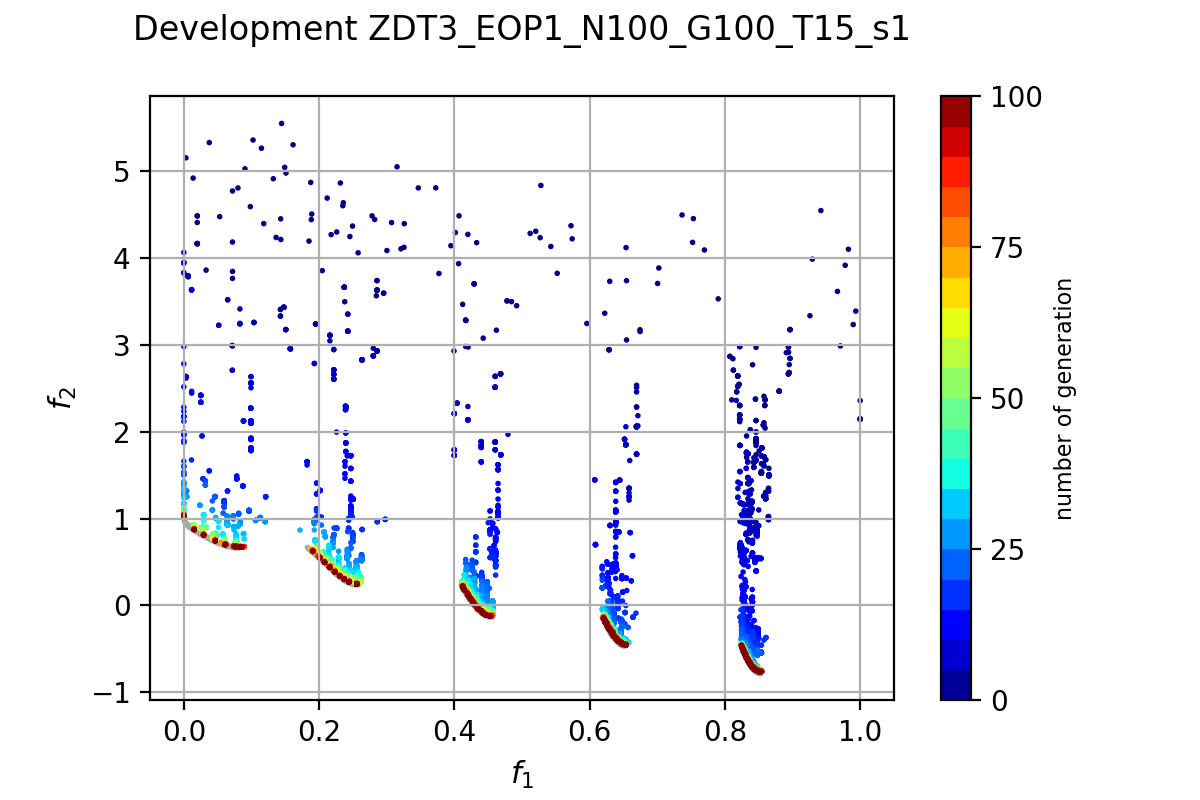
\includegraphics[scale=0.55]{figures/ZDT3_EOP1_N100_G100_T15/s1_dev.png}\\
        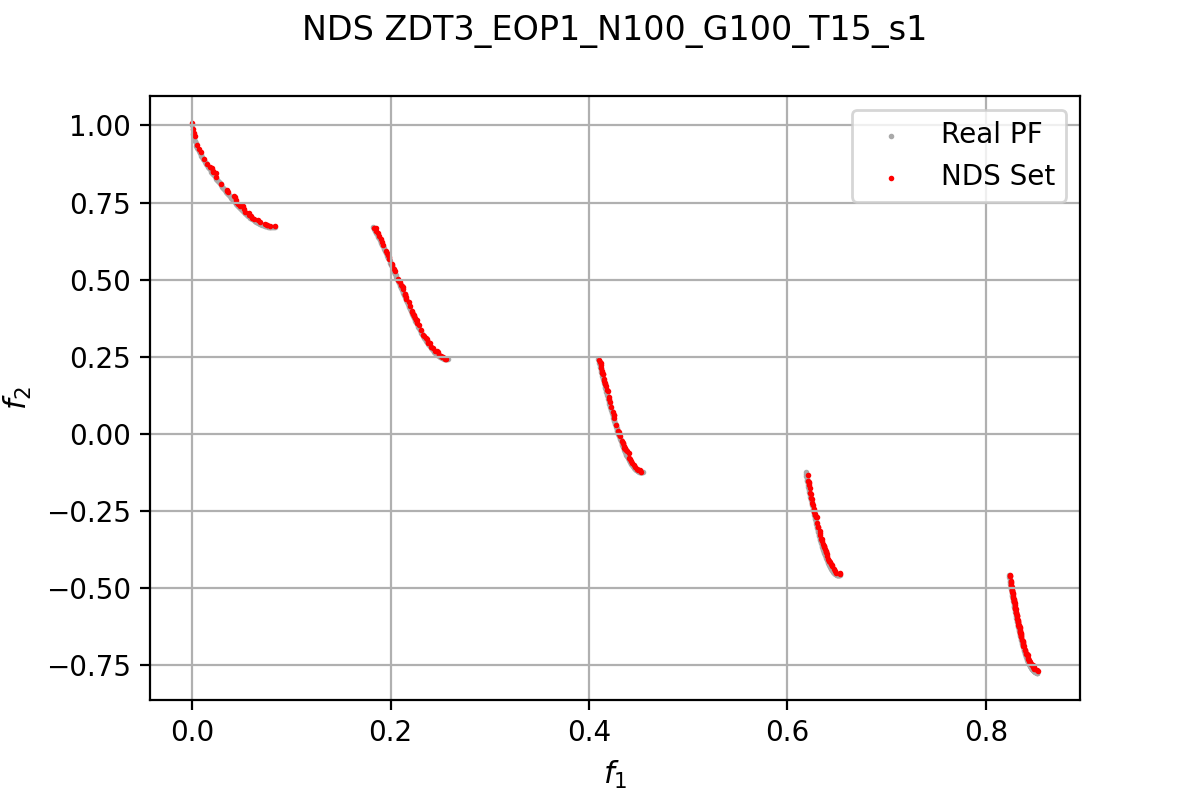
\includegraphics[scale=0.5]{figures/ZDT3_EOP1_N100_G100_T15/s1_nds.png}\\
        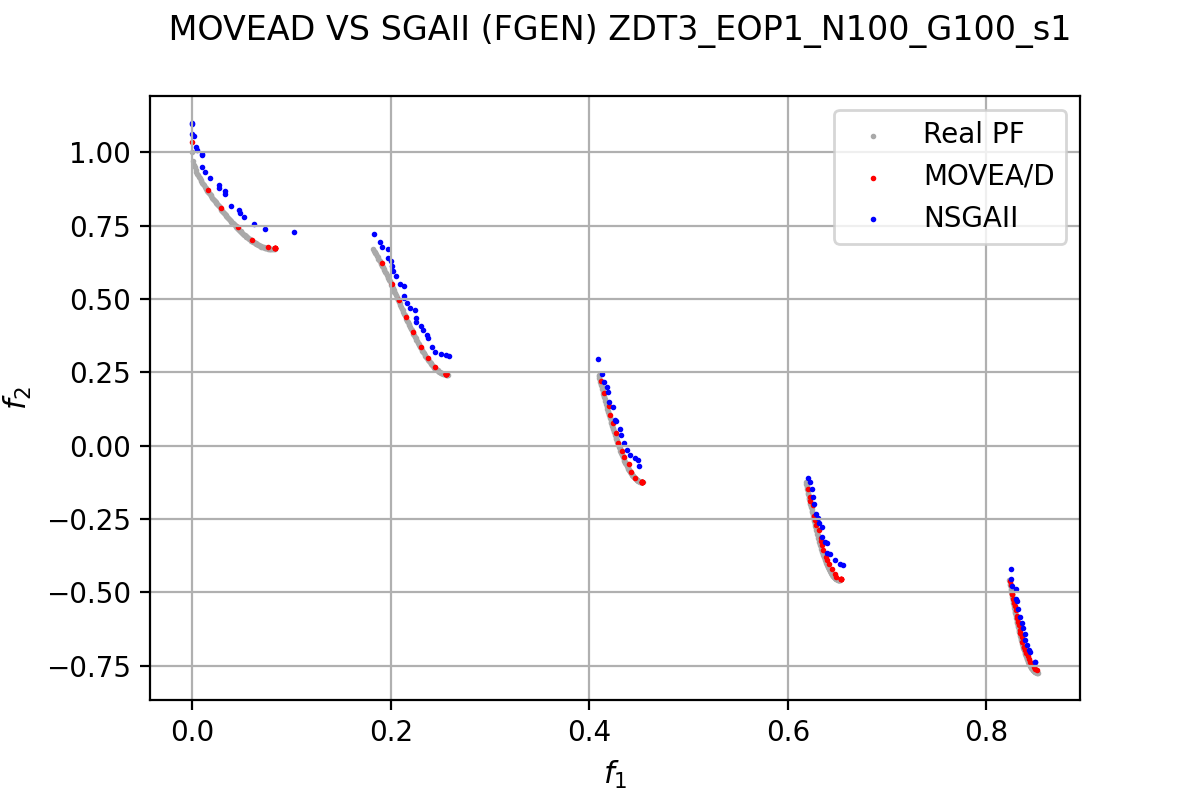
\includegraphics[scale=0.5]{figures/ZDT3_EOP1_N100_G100_T15/s1_comp.png}\\
        \caption{MOEA/D + EOP1 + N100G100}
        \label{fig:2}
    \end{figure}

    \vfill
    \end{minipage}\\

\justify
\subsubsection{Experimentación con 1OOOO ev.}

En este apartado realizamos un estudio (gráfico) del comportamiento del algoritmo, analizando la convergencia y diversidad de la población a lo largo de la ejecución del algoritmo. Propósito de tal estudio es además tratar de esclarecer la influencia de los parámetros $G$ y $N$ en el proceso evolutivo presentando una comparativa de las soluciones finales variando dichos parámetros, manteniendo constante el número de evaluaciontes, para los casos $(G=100, N=100)$, $(G=250, N=40)$ y $(G=50, N=200)$.\\

En la \hyperref[fig:2]{\textit{figura 2}} presentamos tres gráficos pertenecientes a una ejecución característica del algoritmo con el operador evolutivo EOP1, $N=100, G=100$ y $T=15$ (para todos los casos se ha tomado un $15\%$  (recuérdese que en los anexos se muestran varias ejecuciones que validan las discusiones) el primrer diagrama muestra el desarrollo de las soluciones en el espacio de objetivos a lo largo de la ejecución del algoritmo (en las distiontas generaciones). En él podemos apreciar que, tal como esperábamos a medida que el algoritmo avanza (pasan las generaciones) las soluciones tinden a ir convergiendo hacia el frente real de Pareto (señalado en gris), además de forma bastante rápida (los azules corresponden a las primeras generaciones y los anaranjados y rojos a las últimas) de forma que en menos de 50 generaciones se sitúan ya próximas al frente real. Otro aspecto a destacar es la diversidad, en los algoritmos evolutivos es corriente que las soluciones tiendan a concentrarse (se pierde diversidad); en este caso podemos ver dicha tendencia pero al mismo tiempo se puede notar que se tiende a conservar cierta dispersión en los puntos lo que denota una intención de mantener la diversidad (objetivo de todo algoritmo evolutivo).\\

En el segundo diagrama se presenta el conjunto de las soluciones no dominadas calculadas por el algoritmo, que parece corresponder en gran medida con el frente real de pareto, tanto en proximidad (convergencia) como en cobertura (dispersión) en los puntos del frente. Lo que denota, a priori, y a falta de métricas un buen comportamiento del algoritmo. De hecho, esos puntos podrían ser considerados como la salida del algoritmo, esto es la aproximación al frente de pareto que parece ser fiel al frente real (mostrado en gris).\\

Finalmente, presentamos una gráfica comparativa para nuestro algoritmo y para el algoritmo \textit{NSGA-II}. Para ello hemos representado las soluciones en el espacio de objetivos, las cuales corresponden a la última generación de ejecuciones en iguales condiciones $(G=100, N=100)$ para ambos algoritmos. Podemos ver que en cuanto a convergencia (proximidad al frente real) el frente del nuestro algoritmo es sensiblemente mejor que el frente proporcionado por  \textit{NSGA-II} (una gran mayoría de los puntos rojos están por debajo de los azules), mientras que en dispersión parece que los puntos del frente de \textit{NSGA-II} se distribuyen más uniformemente que los de nuestro algoritmo. Pero nótese que si consideramos como salida la proporcionada por el frente de las soluciones no dominadas la tanto la cobertura como la convergencia parecen más que aceptables.\\


Veámos ahora unas gráficas análogas a las presentadas pero para el caso $(G=250, N=40)$ en la \hyperref[fig:3]{\textit{figura 3}} podemos notar que el comportamiento es similar al caso anterior, esto es, como se espera a través de las generaciones las soluciones van aproximándose la convergencia al igual que en el caso anterior sigue siendo es buena, sin embargo se nota que la reducción en el número de subproblemas afecta de manera notable a la dispersión, sobre todo en las últimas generaciones. Sin embargo, si miramos el frente de soluciones no dominadas, vemos que tanto en convergencia (a priori, sin otro algoritmo de referencia) que tanto el grado de convergencia de las soluciones como el grado de dispersión hacen que se aproximen en buena medida al frente real de pareto, por lo que nos incita a pensar que la pérdida de diversidad debe darse relativamente al final porque existen soluciones buenas a lo largo prácticamente de todo el frente. Si comparamos ahora la última generación con la del algoritmo \textit{NSGA-II} (ejecutado en las mismas condiciones) podemos ver que ahora la superioridad no es tan patente como en el casi anterior y ambos algoritmos alcanzan un grado análogo de convergencia y dispersión (en este último aspecto quizá \textit{NSGA-II} parezca un poco mejor).\\

\begin{minipage}[H]{0.47\linewidth}
\begin{figure}[H]
        \centering
        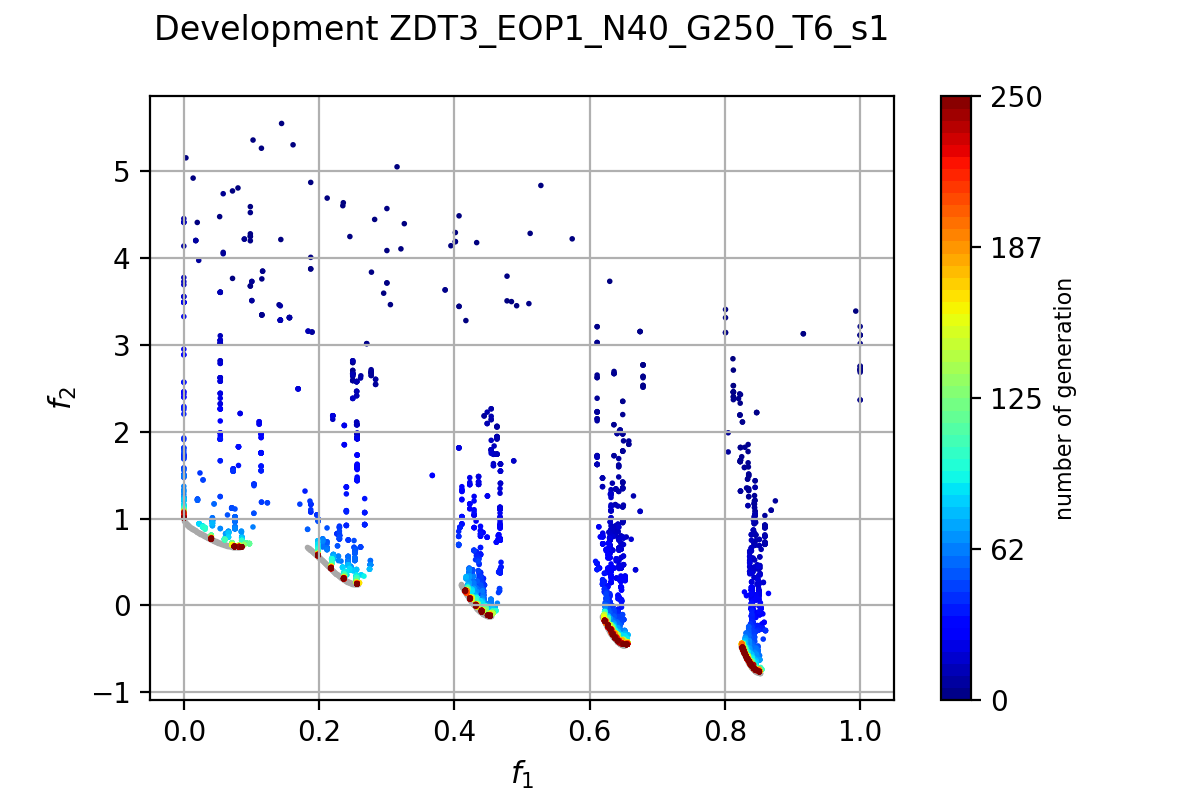
\includegraphics[scale=0.55]{figures/ZDT3_EOP1_N40_G250_T6/s1_dev.png}\\
        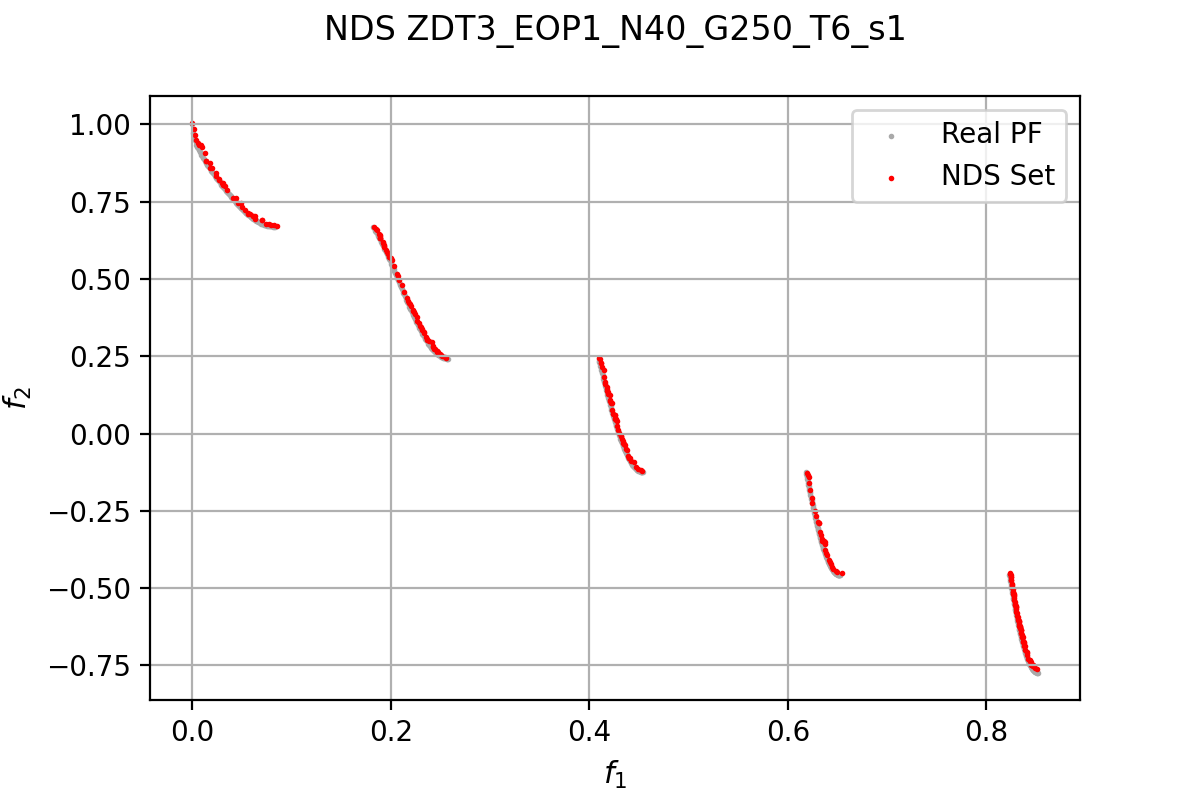
\includegraphics[scale=0.5]{figures/ZDT3_EOP1_N40_G250_T6/s1_nds.png}\\
        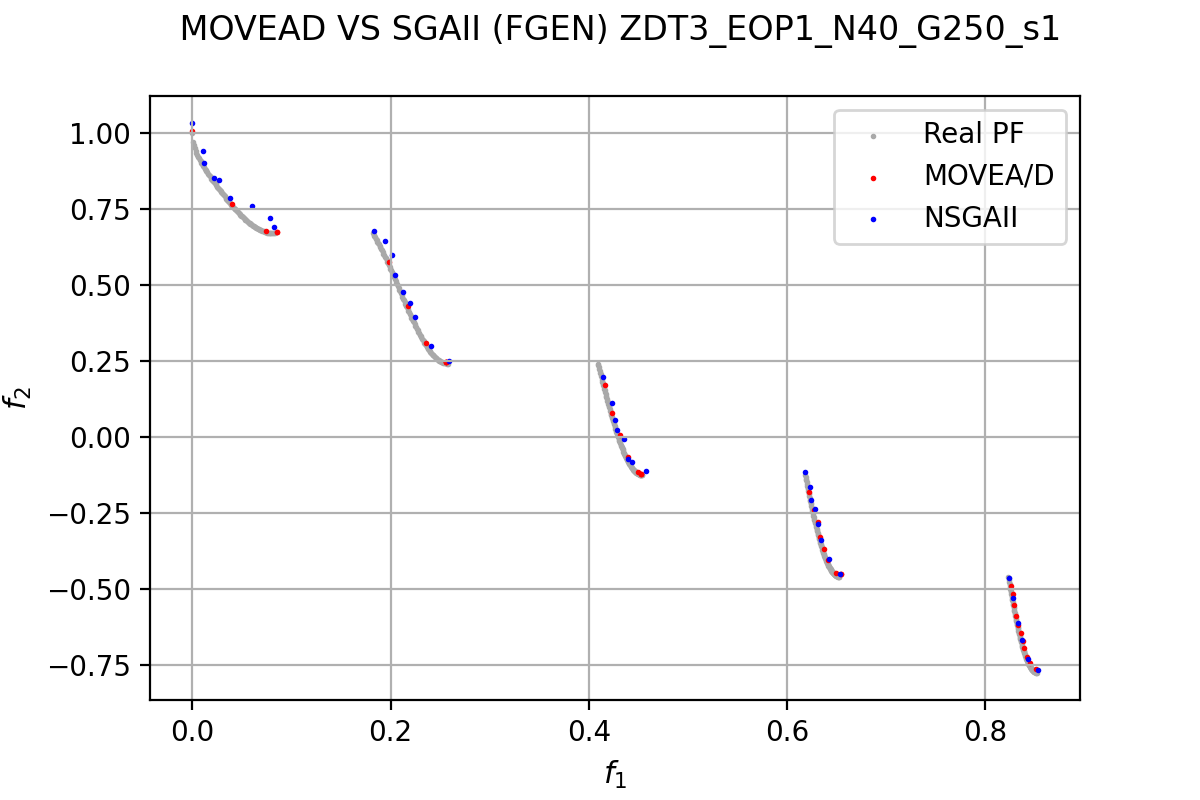
\includegraphics[scale=0.5]{figures/ZDT3_EOP1_N40_G250_T6/s1_comp.png}\\
        \caption{MOEA/D + EOP1 + N40G250}
        \label{fig:3}
    \end{figure}
\end{minipage} \hfill
\begin{minipage}[H]{0.47\linewidth}
    \begin{figure}[H]
        \centering
        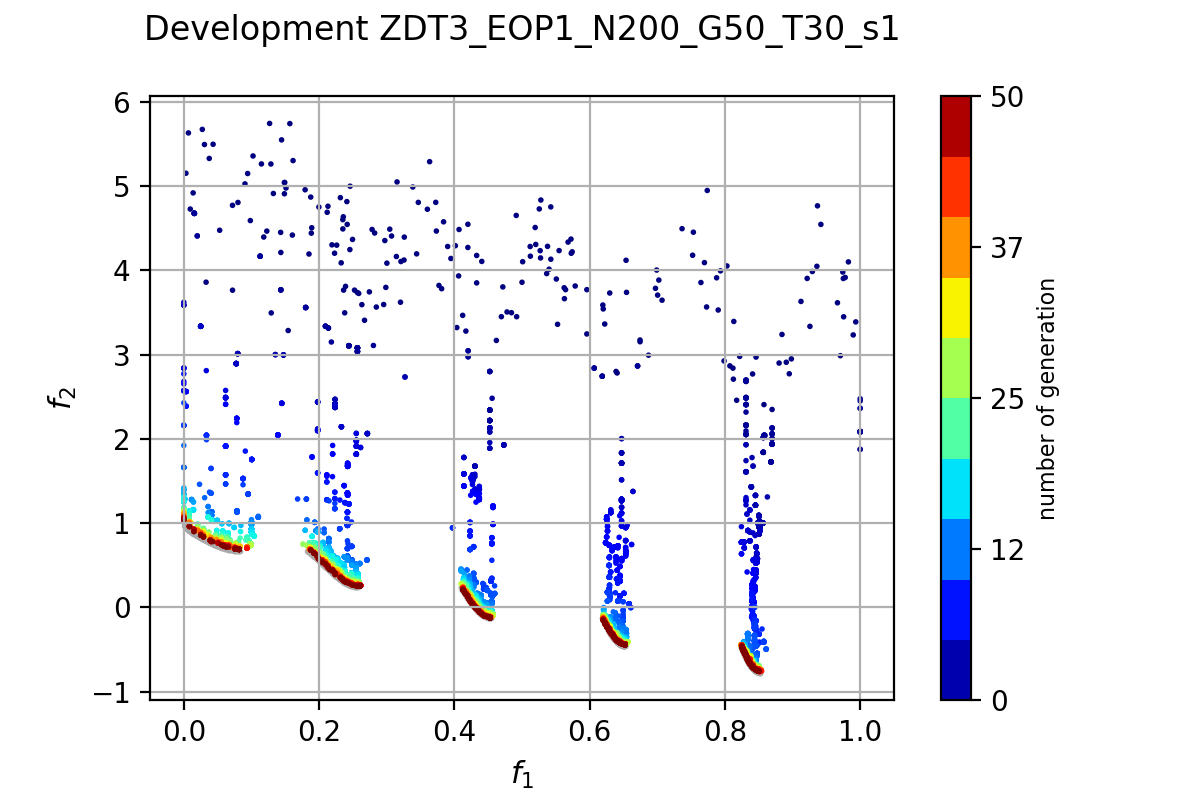
\includegraphics[scale=0.55]{figures/ZDT3_EOP1_N200_G50_T30/s1_dev.png}\\
        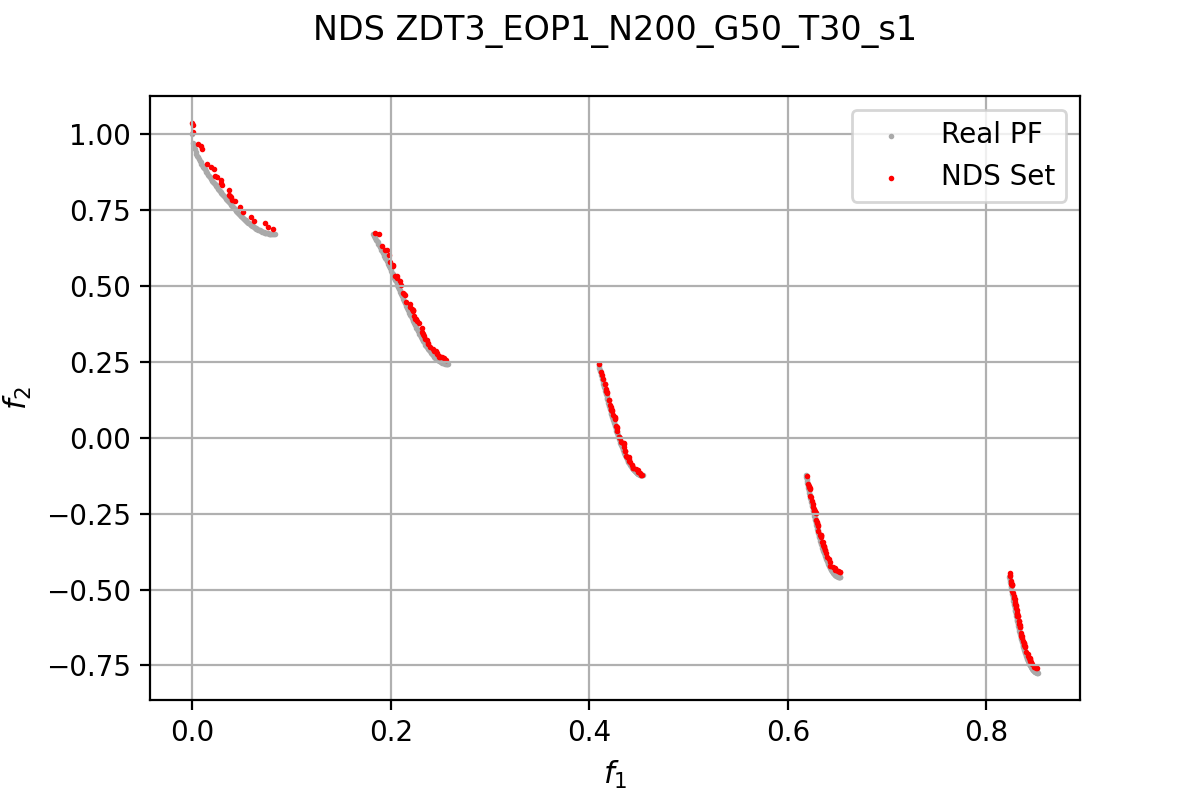
\includegraphics[scale=0.5]{figures/ZDT3_EOP1_N200_G50_T30/s1_nds.png}\\
        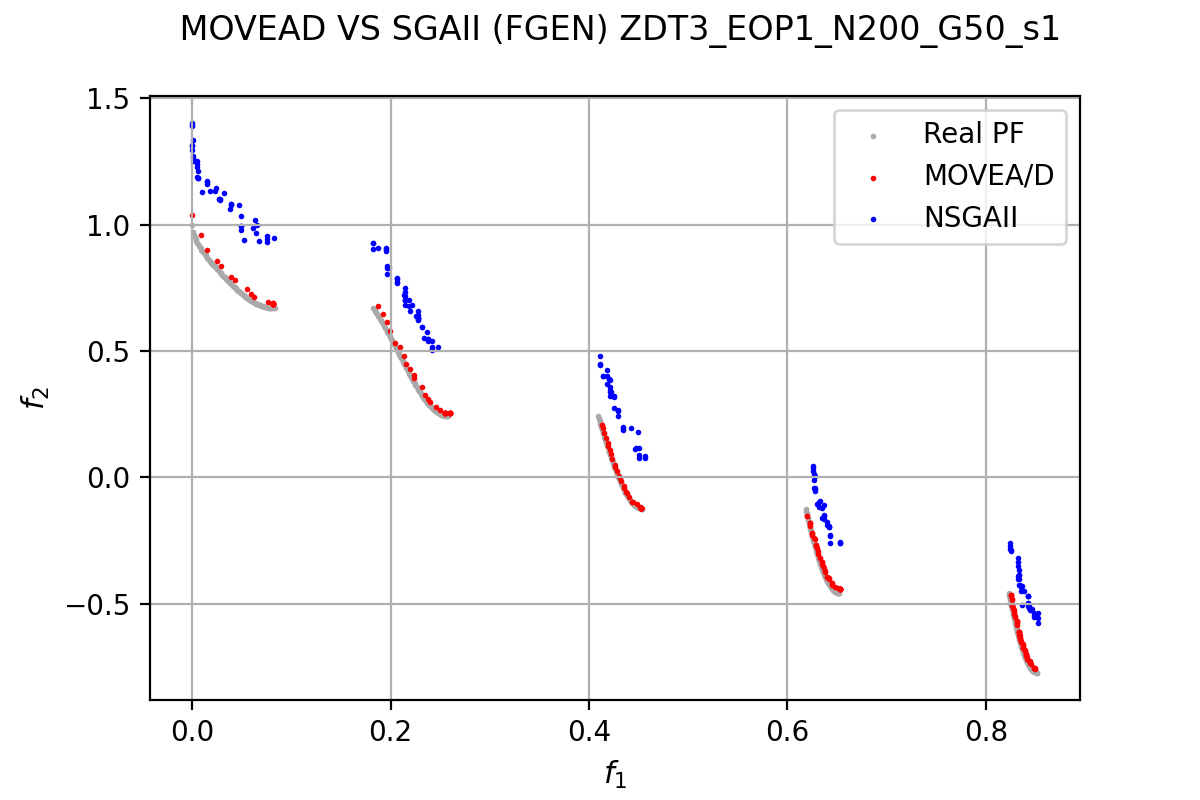
\includegraphics[scale=0.5]{figures/ZDT3_EOP1_N200_G50_T30/s1_comp.png}\\
        \caption{MOEA/D + EOP1 + N200G50}
        \label{fig:4}
    \end{figure}

    \vfill
    \end{minipage}\\


Y en último lugar comprobemos cuál es el resultado de elevar el número de subproblemas frente al número de generaciones. Dado que según hemos visto hasta ahora lo convergencia suele ser rápida, y que el número de subproblemas favorecerá la diversidad, a priori el comportamiento debería ser satisfactorio. Veámos qué ocurre para el caso $(G=250, N=40)$ en las gráficas presentadas en la \hyperref[fig:4]{\textit{figura 4}}. Podemos notar que la convergencia es bastante buena y la diversidad también permite que en las últimas generaciones se cubran los tramos del frente de manera más o menos uniforme. De hecho, si observamos el diagrama de las soluciones no dominadas podemos notar que, primero el ajuste es ligeramente peor que en los otros casos (normal dado que tiene menos generaciones para tratar de ajustarse) y la cobertura es buena y se reparte de forma más o menos uniforme. Si comparamos con la ejecución del \textit{NSGA-II} en este caso nuestro algoritmo es claramente mejor en convergencia y también algo mejor en cobertura (tramos más largos). \\

Finalmente vamos a realizar una comparativa entre los tres casos tanto para los frentes de la última generación como para los frentes \textit{NSD}. En la \hyperref[fig:5]{\textit{figura 5}} se muestran las dos gráficas de comparativa de los frente anteriormente indicados. En cuanto a las soluciones de la generación final todas se encuentran bastante superpuestas, quizá la roja con con una ligera menor convergencia (proximidad al frente) y la verde con una menor convergencia pudiendo ser la azul la más adecuada, esto es un balance en el número de generaciones y número de subproblemas lo que proporciona la mejor solución, aunque los resultados no son concluyentes y trataremos de realizar un estudio más profundo con el uso de las métricas. \\

En cuanto al NSD, las sensaciones son similares se nota bastante superposición entre los puntos, quizá con la roja un poco menor de convergencia en algunas partes y la azul y la verde muy similares, los resultados no son nada concluyentes, así que intentaremos clarificarlos con el uso de métricas y el correspondiente estudio estadístico de las mismas. 

\begin{center}
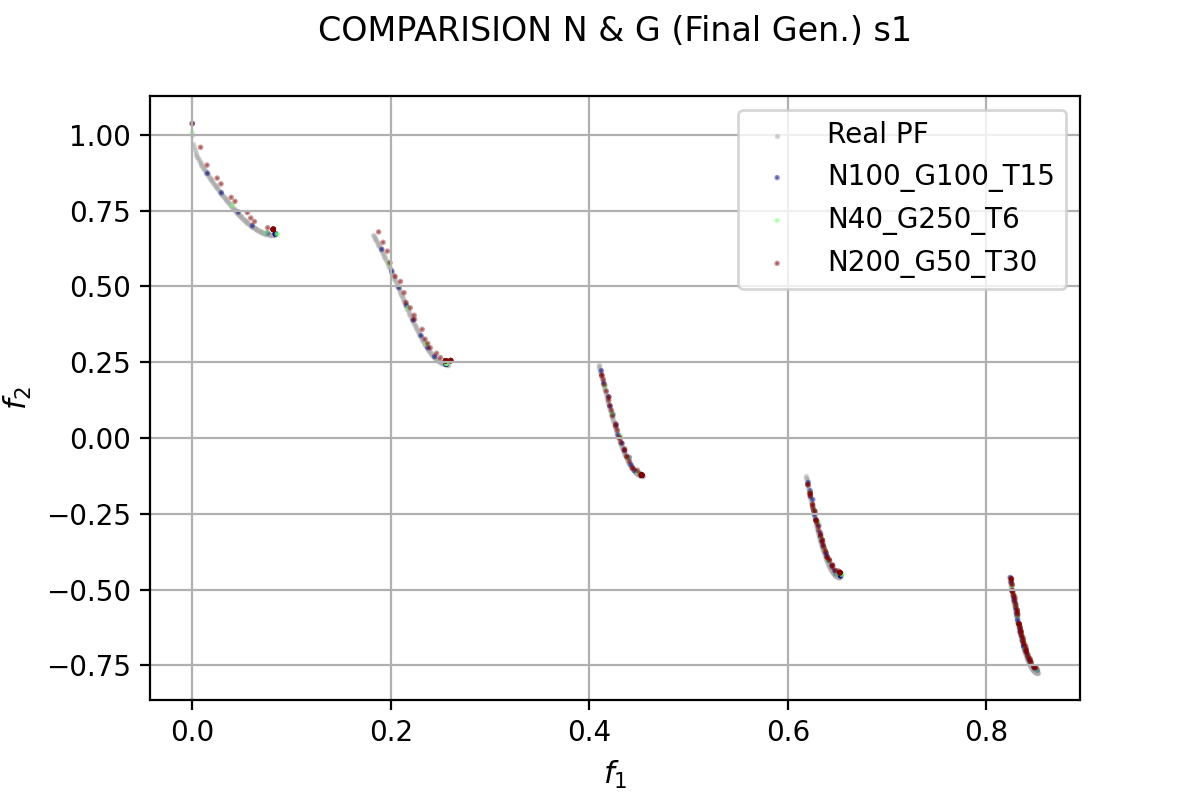
\includegraphics[scale=0.9]{figures/COMPARISIONS_EOP1/GCOMP_FGEN_s1.png}\\
\end{center}
\begin{figure}[H]
\centering
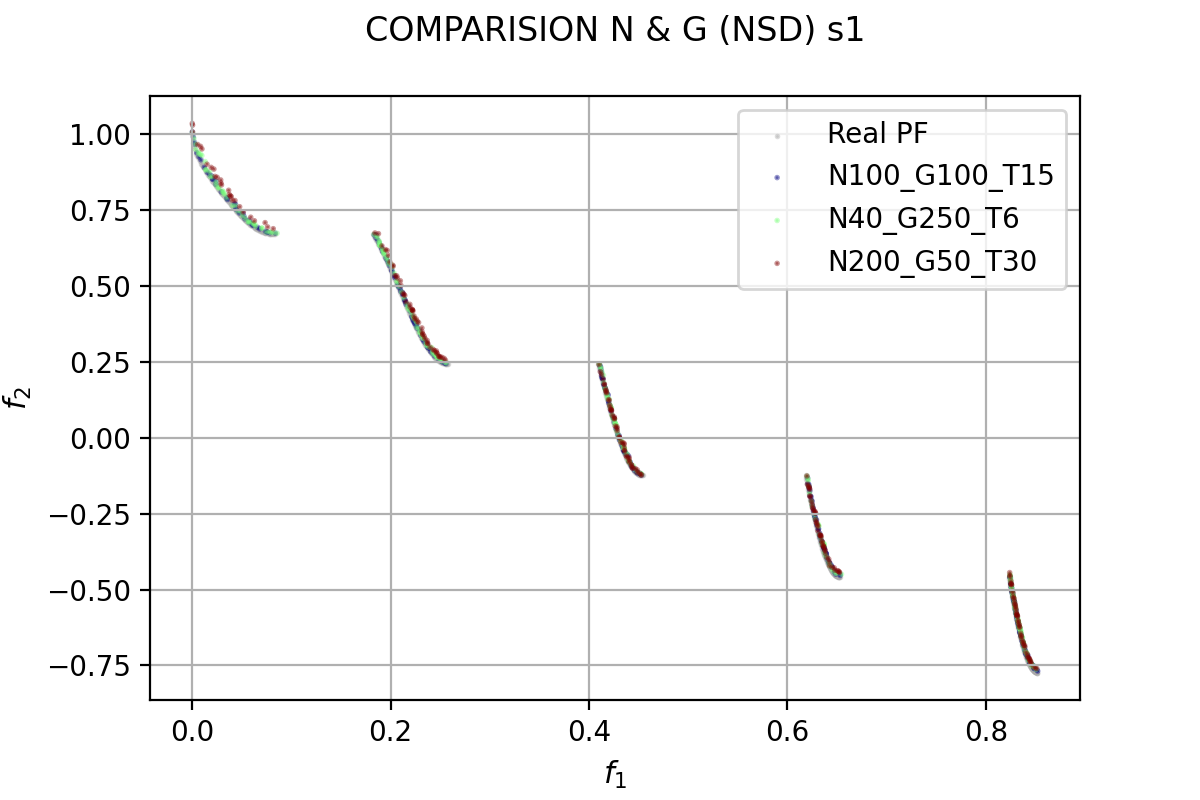
\includegraphics[scale=0.9]{figures/COMPARISIONS_EOP1/GCOMP_NDS_s1.png}\\
\caption{MOEA/D + EOP1. Comparación de casos}
\label{fig:5}
\end{figure}



\subsubsection{Análisis de métricas para 10000 ev.}

Presentado el estudio preliminar anterior vamos a tratar de profundizar para exclarecer y llevar a cabo una discusión más profunda de los casos anteriores. Para ello realizaremos un estudio de algunas métricas para los casos ya presentados. Tales métricas corresponden al hipervolumen, espaciado y cover set.\\

Comencemos viendo algunas gráficas asociadas a las métricas para los casos planteados en el apartado anterior. En la \hyperref[fig:6]{figura 6} se muestra la evolución de hipervolumen y el espaciado en durante las distintas generaciones para 10 ejecuciones del algoritmo. Podemos observar que en todos los casos  el desarrollo del hipervolumen como el del espaciado se comportan de manera bastante uniforme para todas las generaciones, lo que denota que nuestro algoritmo es robusto (aunque, lógicamente, dos ejecuciones distintas tienen comportamientos distintos, dado el carácter estocástico del algoritmo). Aunque no es posible hacer un análisis conjunto del hipervolumen (ya que el punto de referencia para su cálculo es distinto en cada caso) sí podemos destacar la rápida convergencia del algoritmo (que destacamos también en el estudio preliminar) y el aparente estancamiento final, por lo que es preferible primar el número de subproblemas frente al número de generaciones (en valores razonables)como sugiere también el comportamiento del espaciado.\\


\begin{figure}[H]
\centering
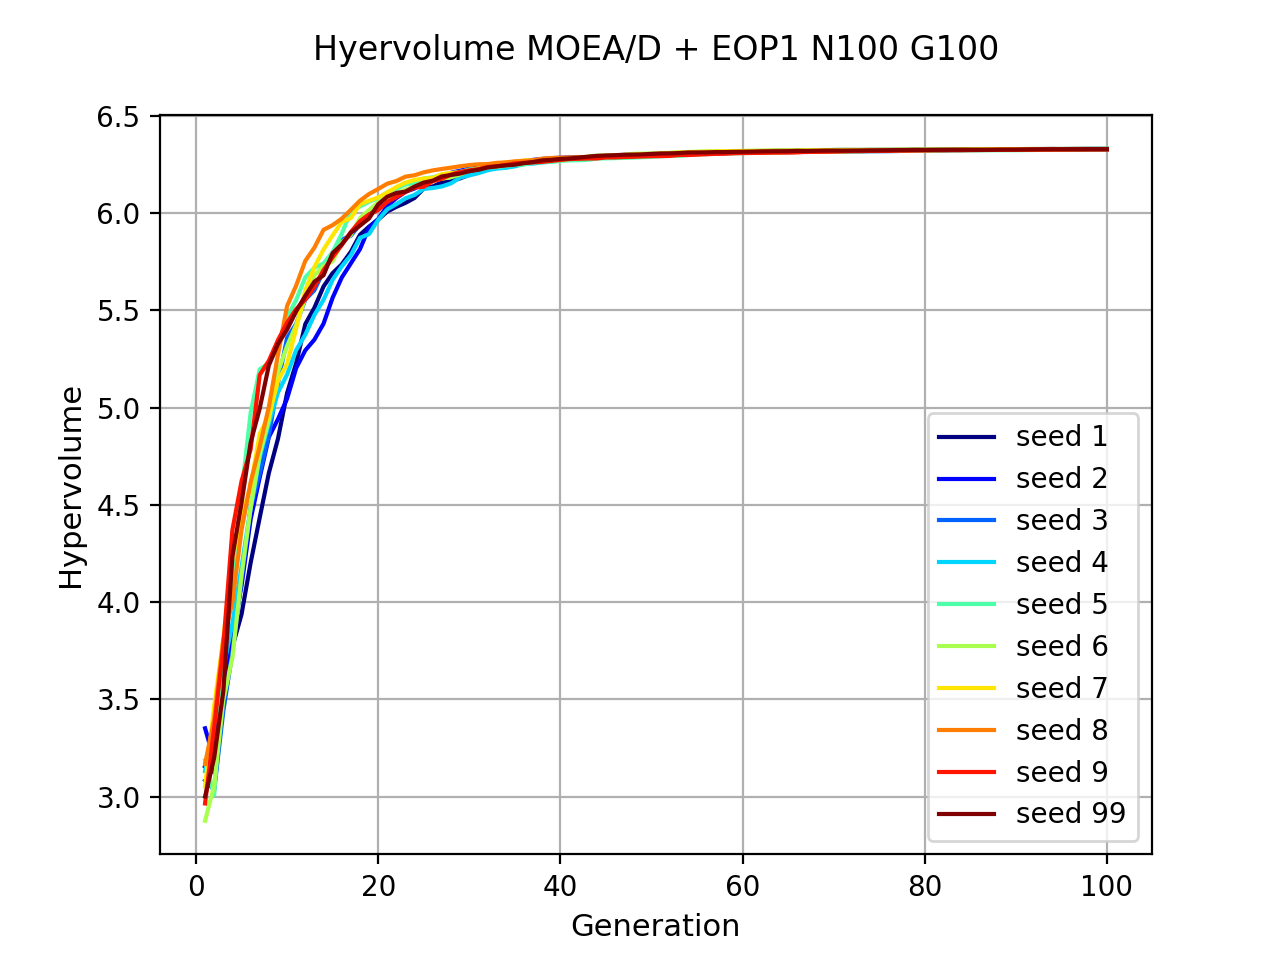
\includegraphics[scale=0.5]{figures/METRICS_EOP1/Hypervol_N100_G100.png} \quad 
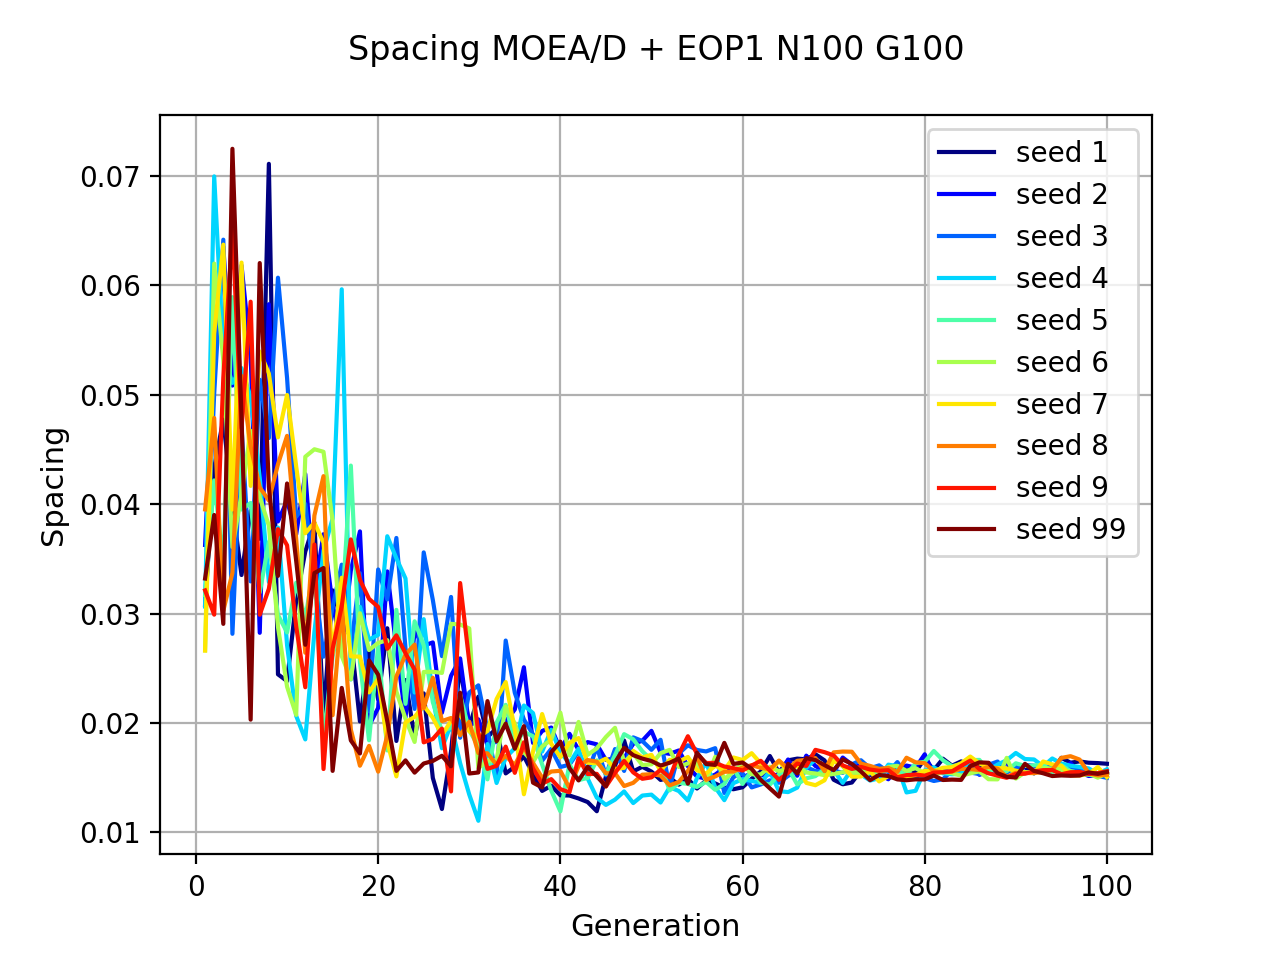
\includegraphics[scale=0.5]{figures/METRICS_EOP1/Spacing_N100_G100.png}\\
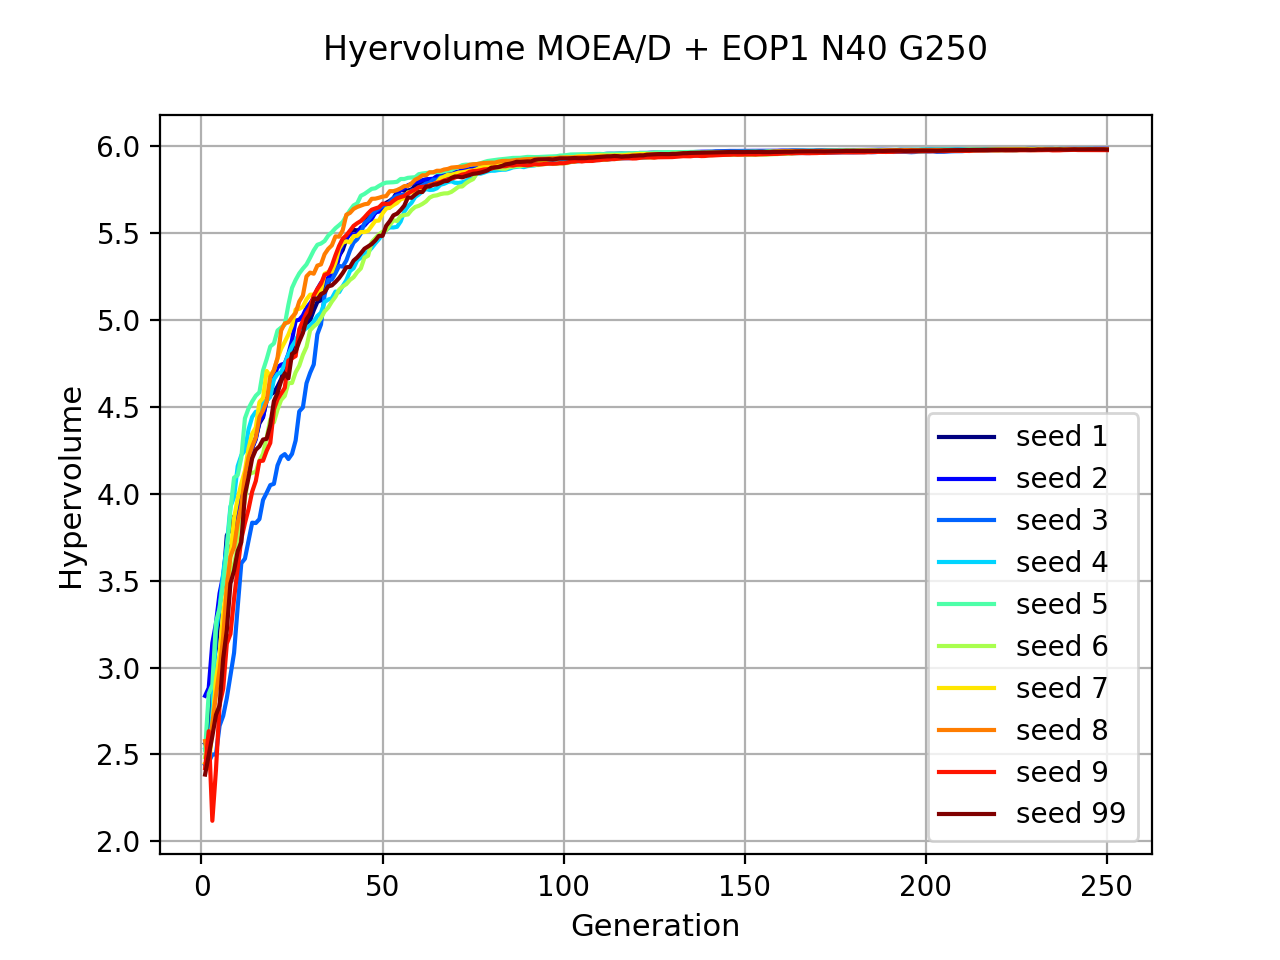
\includegraphics[scale=0.5]{figures/METRICS_EOP1/Hypervol_N40_G250.png}\quad 
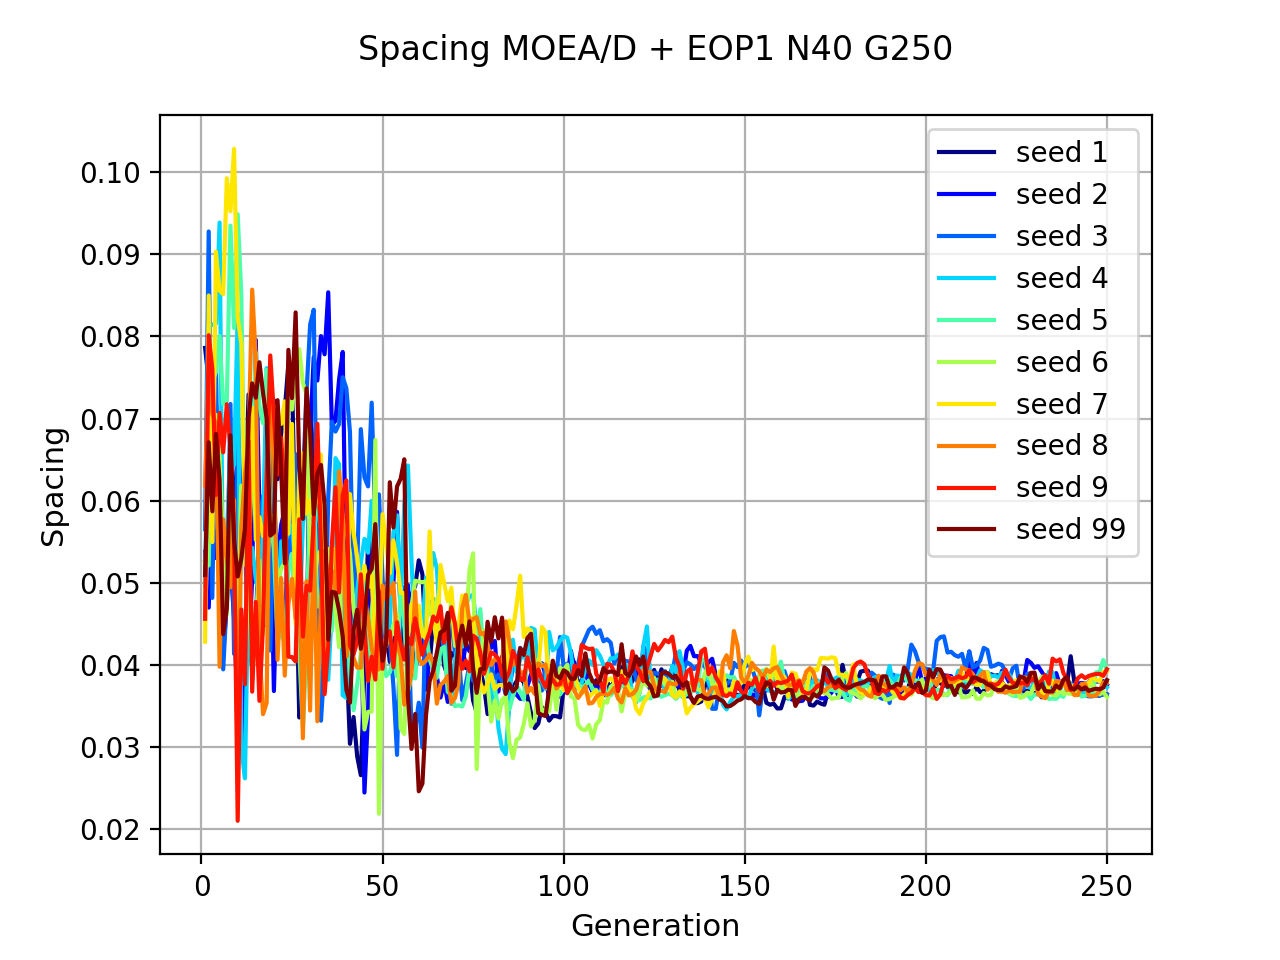
\includegraphics[scale=0.5]{figures/METRICS_EOP1/Spacing_N40_G250.png}\\
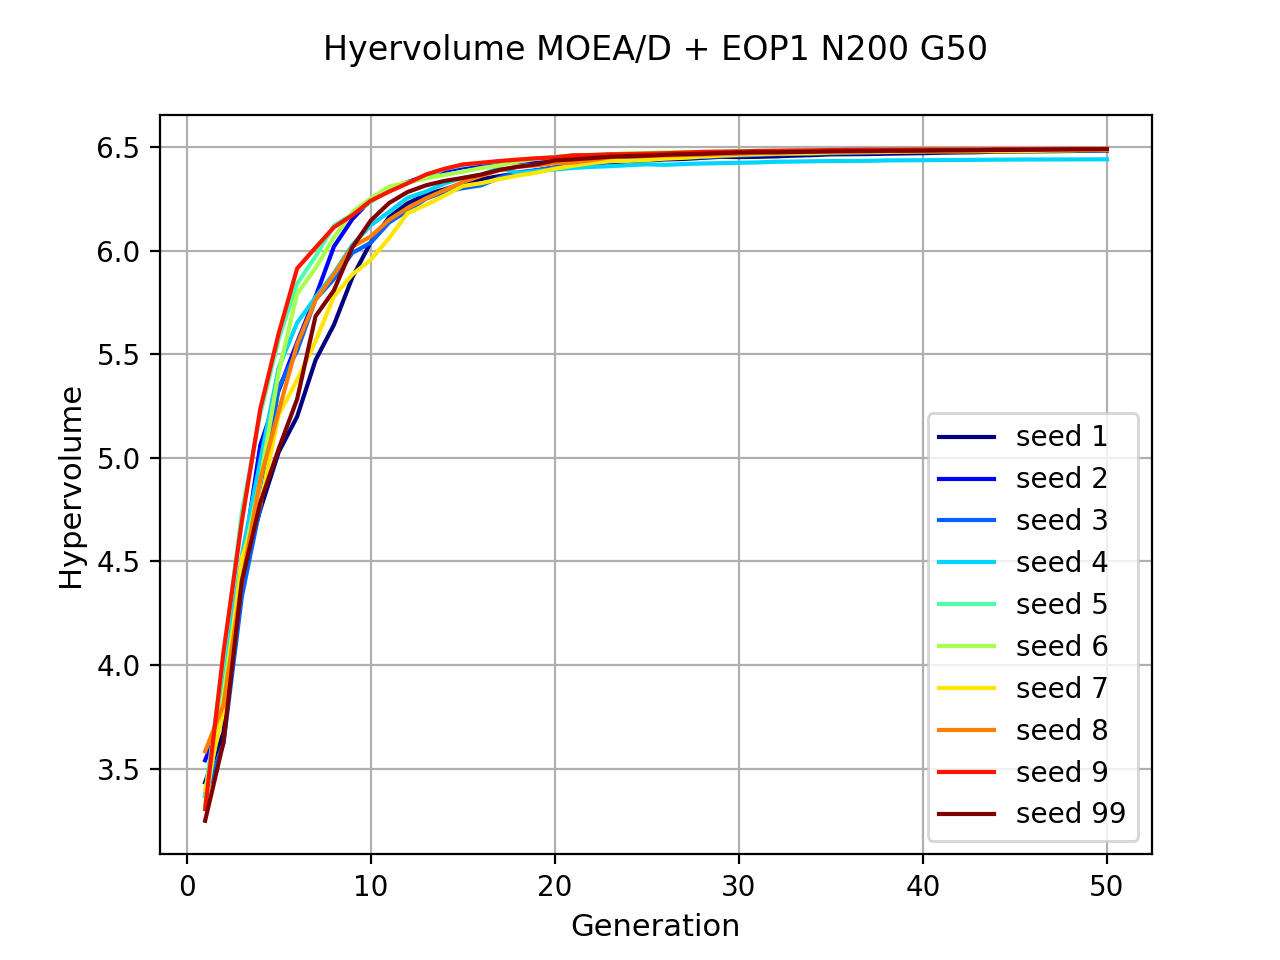
\includegraphics[scale=0.5]{figures/METRICS_EOP1/Hypervol_N200_G50.png}\quad 
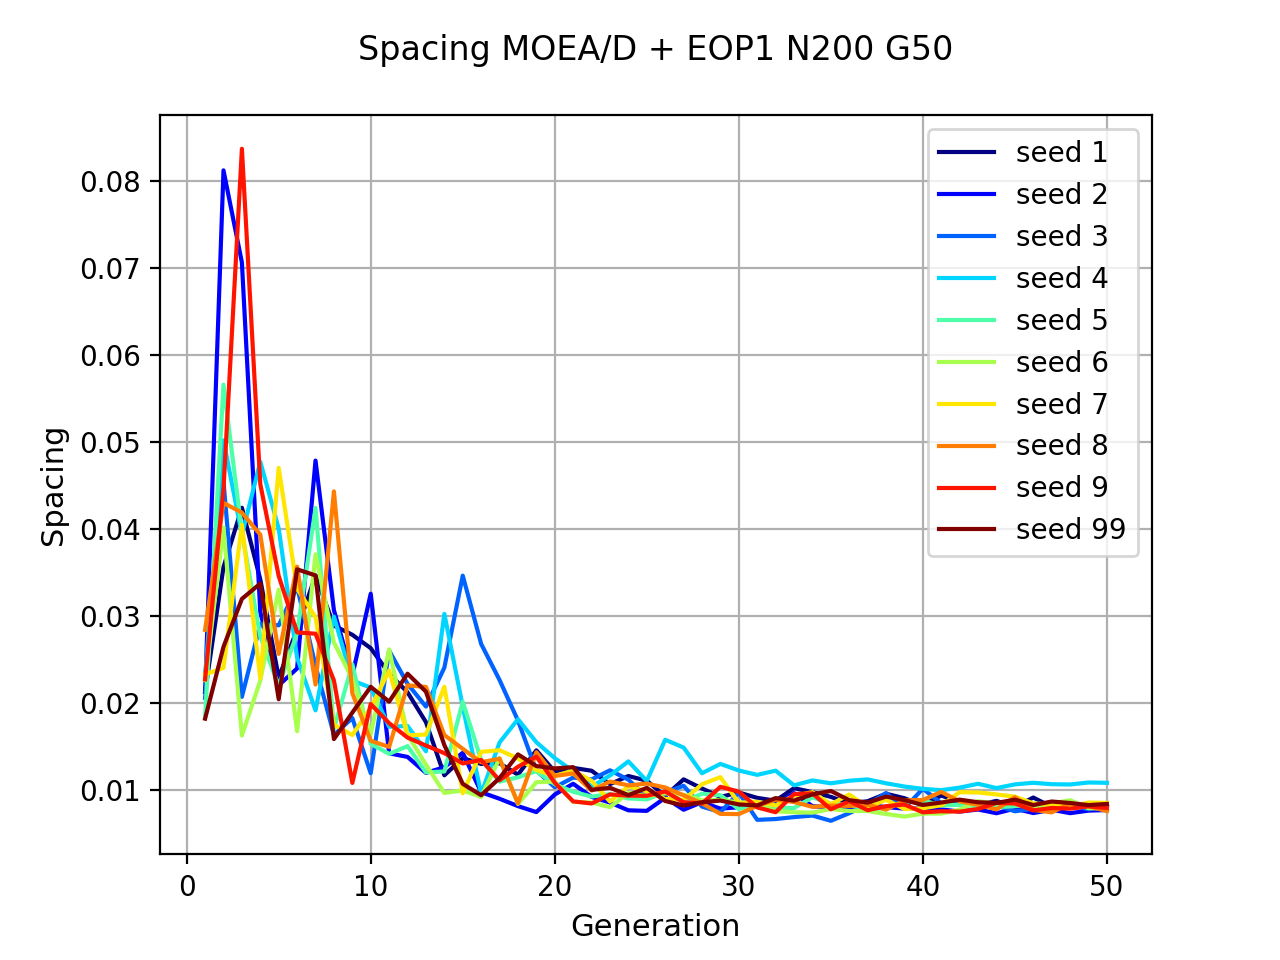
\includegraphics[scale=0.5]{figures/METRICS_EOP1/Spacing_N200_G50.png}\\
\caption{MOEA/D + EOP1. Méticas para 10000 EV}
\label{fig:6}
\end{figure}

A continuación presentaremos algunas gráficas comparativas del comportamiento del algoritmo frente a \textit{NSGAII}. En la \hyperref[fig:7]{figura 7} se muestran las graficas con dichas comparativas en las que podemos notar que en todos los casos el espaciado en el algoritmo NSGAII se compora mejor que en algoritmo propuesto mientras que el hipervolumen suele ser al revés. Como vimos en el estudio preliminar el algoritmo sí suele converger a soluciones mejores que el algoritmo \textit{NSGAII} pero también suele tender a concentrar más las soluciones. Sin embargo si comprobamos la métrica cover set, sí podemos ver que para el segundo y el tercer caso ($N100$ y $N200$) el algoritmo propuesto tiende a dominar al \textit{NSGAII}, para el primer caso en todas las ejecuciones el frente del algoritmo \textit{NSGAII} quedó dominado por el de \textit{MOEA/D + EOP1} en más del 80\% de sus puntos, mientras que el frente de  \textit{NSGAII} no es apreciable que dominase al \textit{MOEA/D + EOP1} en ni siquiera un 2\% en niguna de las ejecuciones; y además este comportamiento es patente a partir las 5 primeras iteraciones. No es así para el caso $N=40$, en el que el nuestro algorito sí supera en hipervolumen al \textit{NSGAII} pero es sensiblemente peor en cuanto al espaciado y en cuanto al cover set en ningún caso ninguno de los dos frentes es dominado más de un 40\% por el otro. aunque nuestro algoritmo tienda a quedear por debajo. Como venimos repitiendo a nuestro algoritmo le aporta más un número alto de subproblemas que de generaciones.


\begin{figure}[H]
\centering
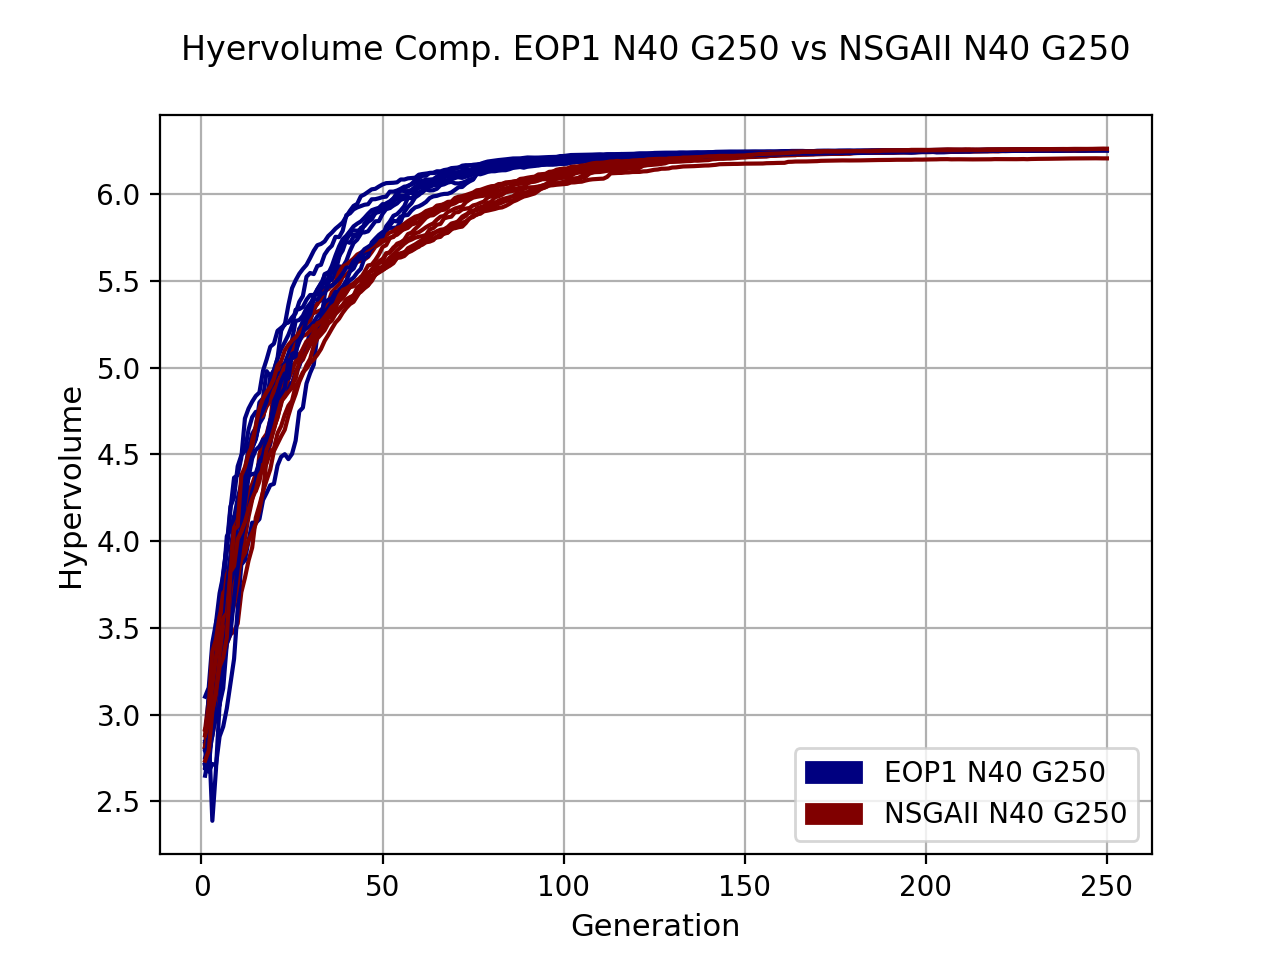
\includegraphics[scale=0.35]{../METRICS_PLOTS/Hypervol_COMP_EOP1N40G250_NSGAIIN40G250.png}
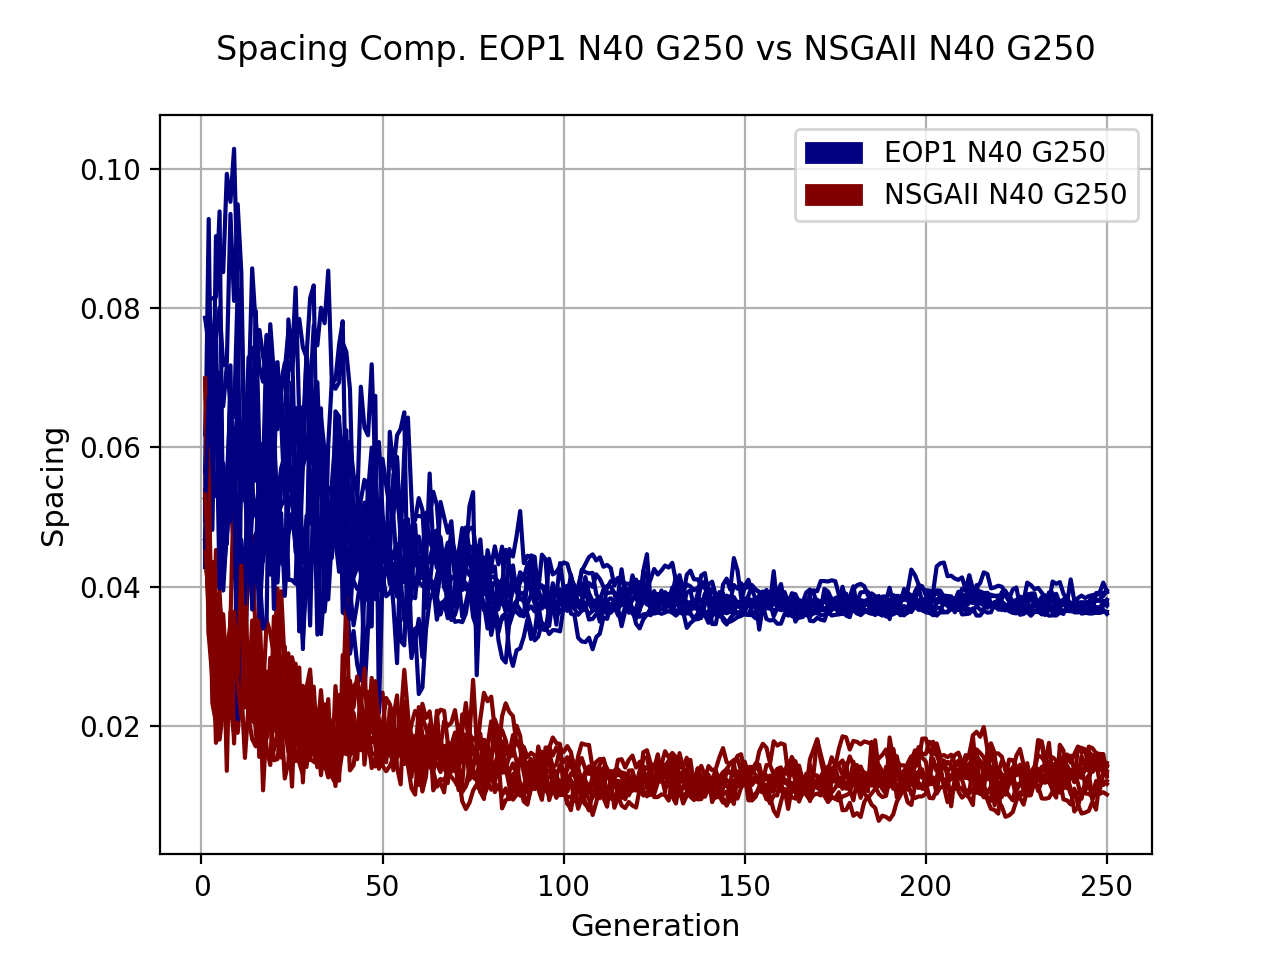
\includegraphics[scale=0.35]{../METRICS_PLOTS/Spacing_COMP_EOP1N40G250_NSGAIIN40G250.png}
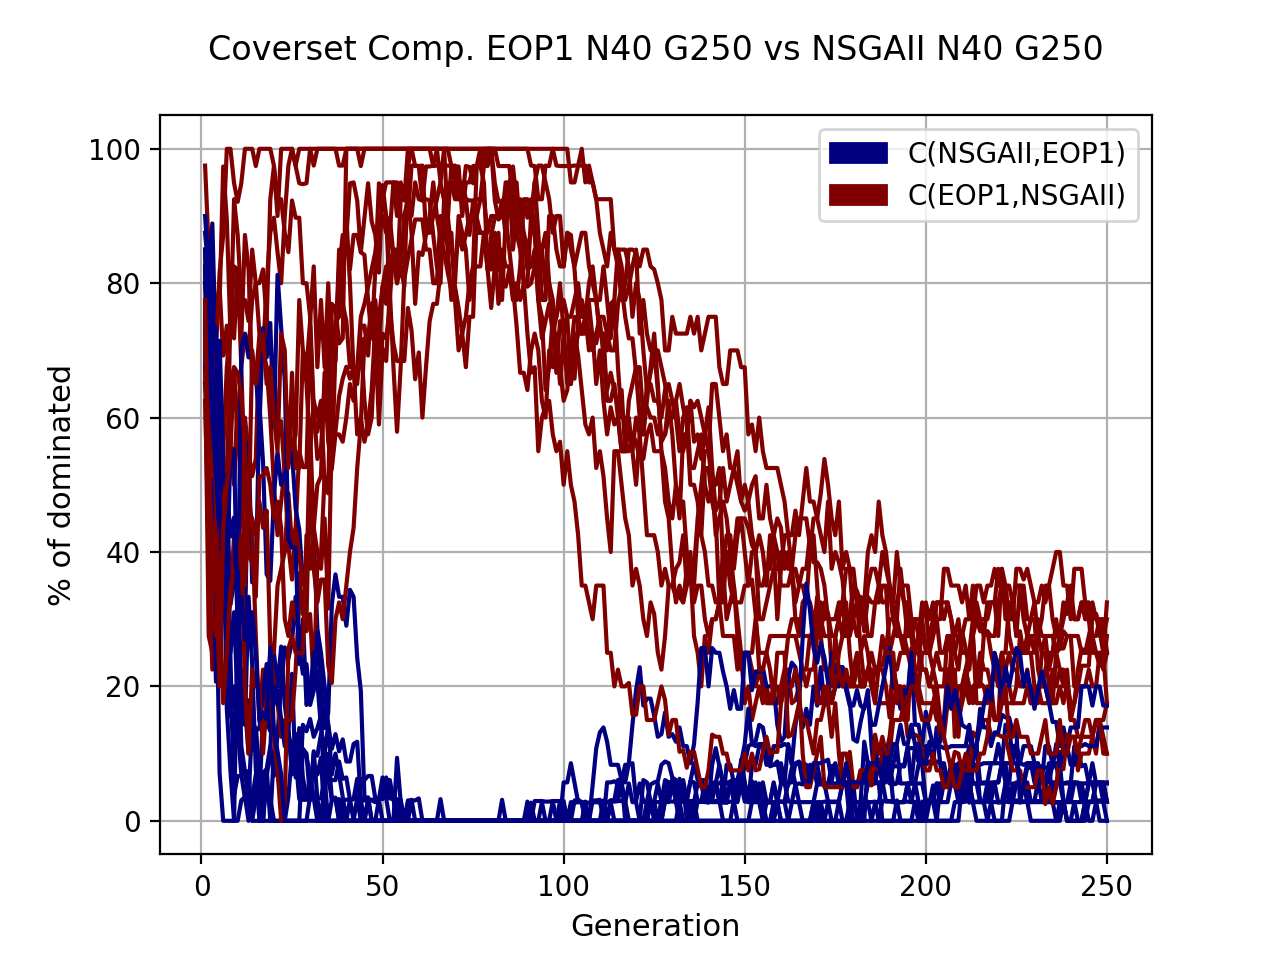
\includegraphics[scale=0.35]{../METRICS_PLOTS/CoverSet_COMP_EOP1N40G250_NSGAIIN40G250.png}\\
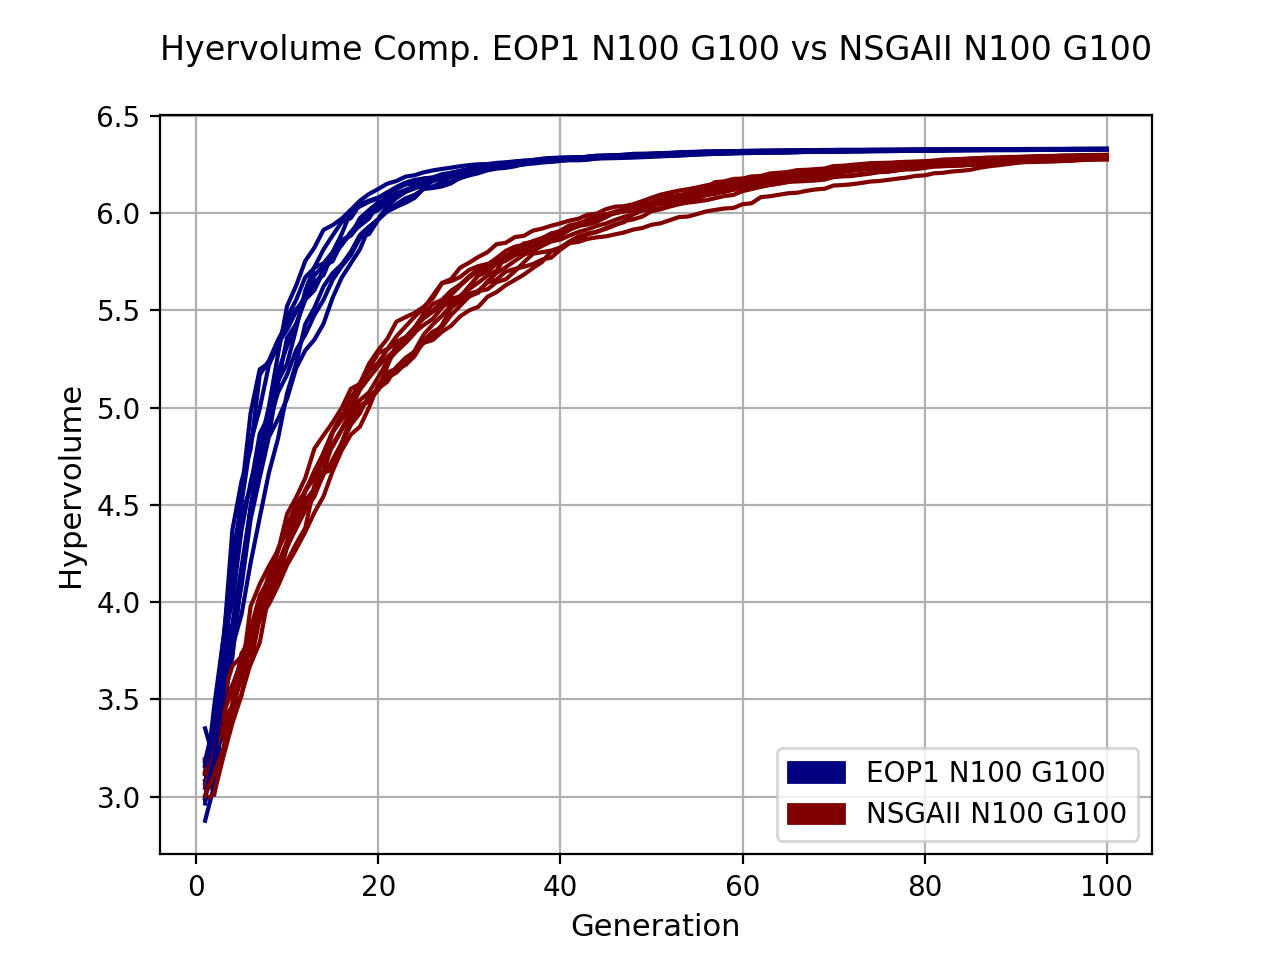
\includegraphics[scale=0.35]{../METRICS_PLOTS/Hypervol_COMP_EOP1N100G100_NSGAIIN100G100.png}
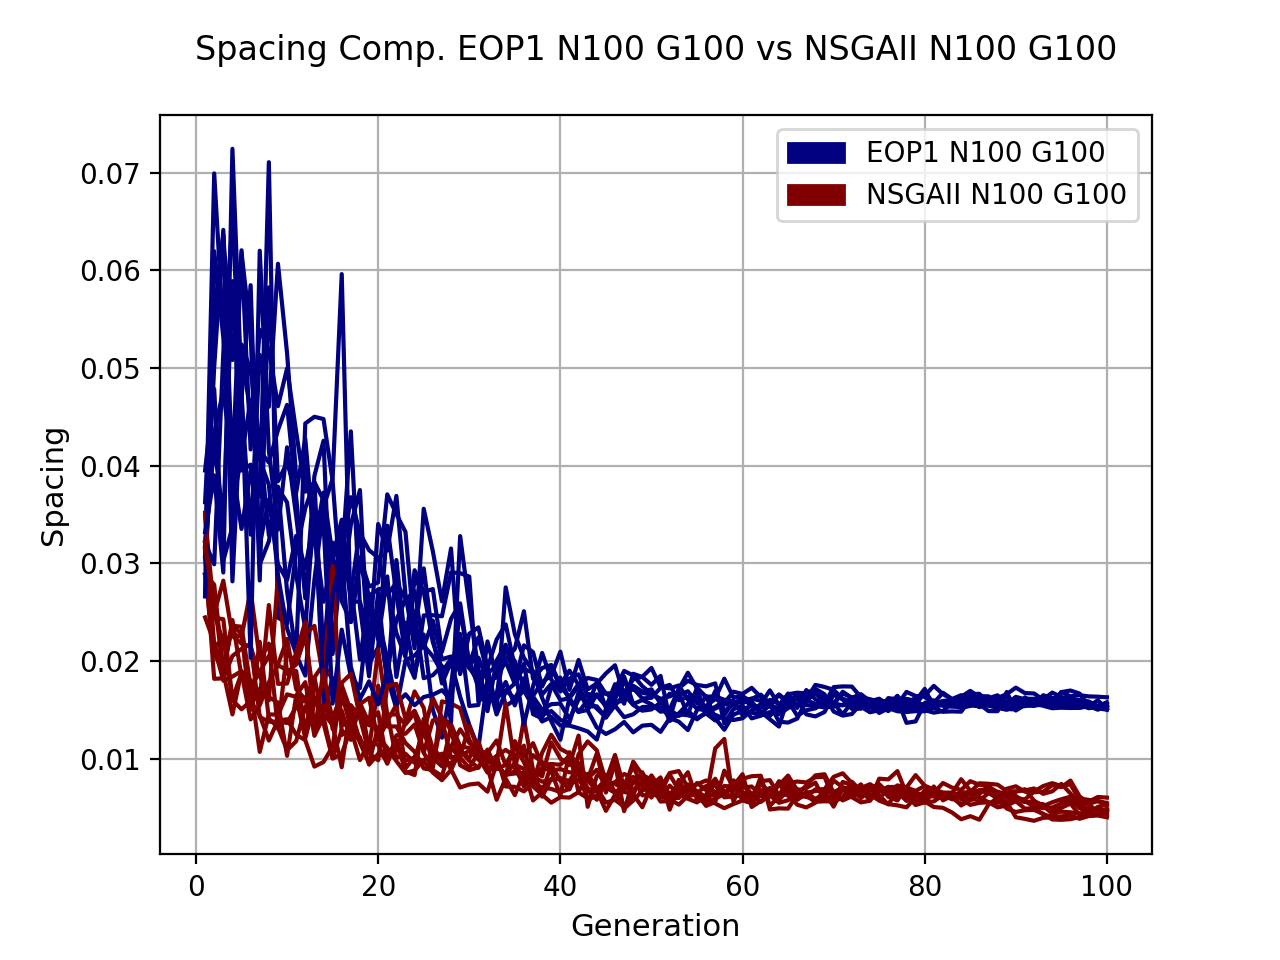
\includegraphics[scale=0.35]{../METRICS_PLOTS/Spacing_COMP_EOP1N100G100_NSGAIIN100G100.png}
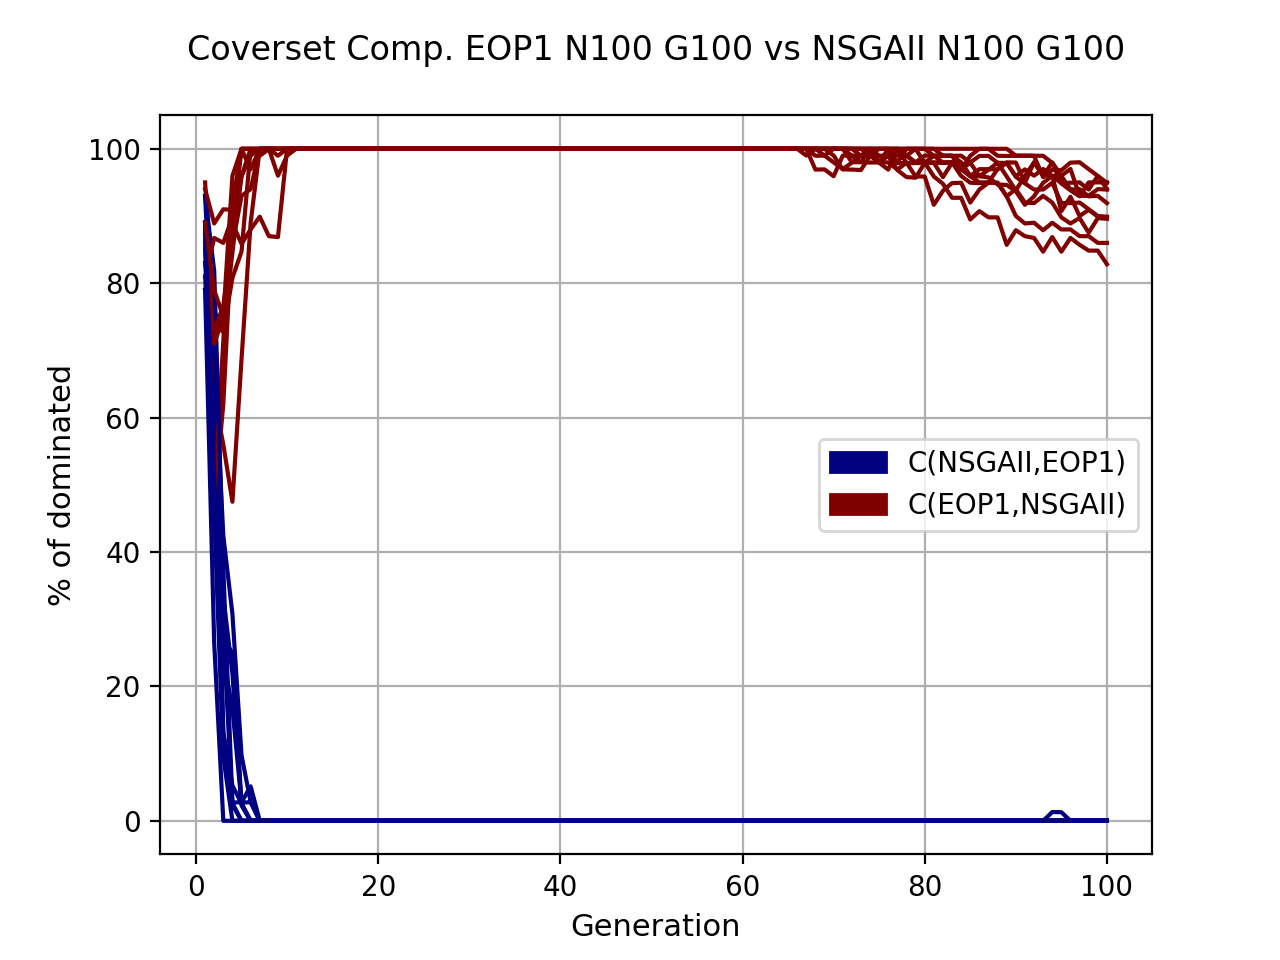
\includegraphics[scale=0.35]{../METRICS_PLOTS/CoverSet_COMP_EOP1N100G100_NSGAIIN100G100.png}\\
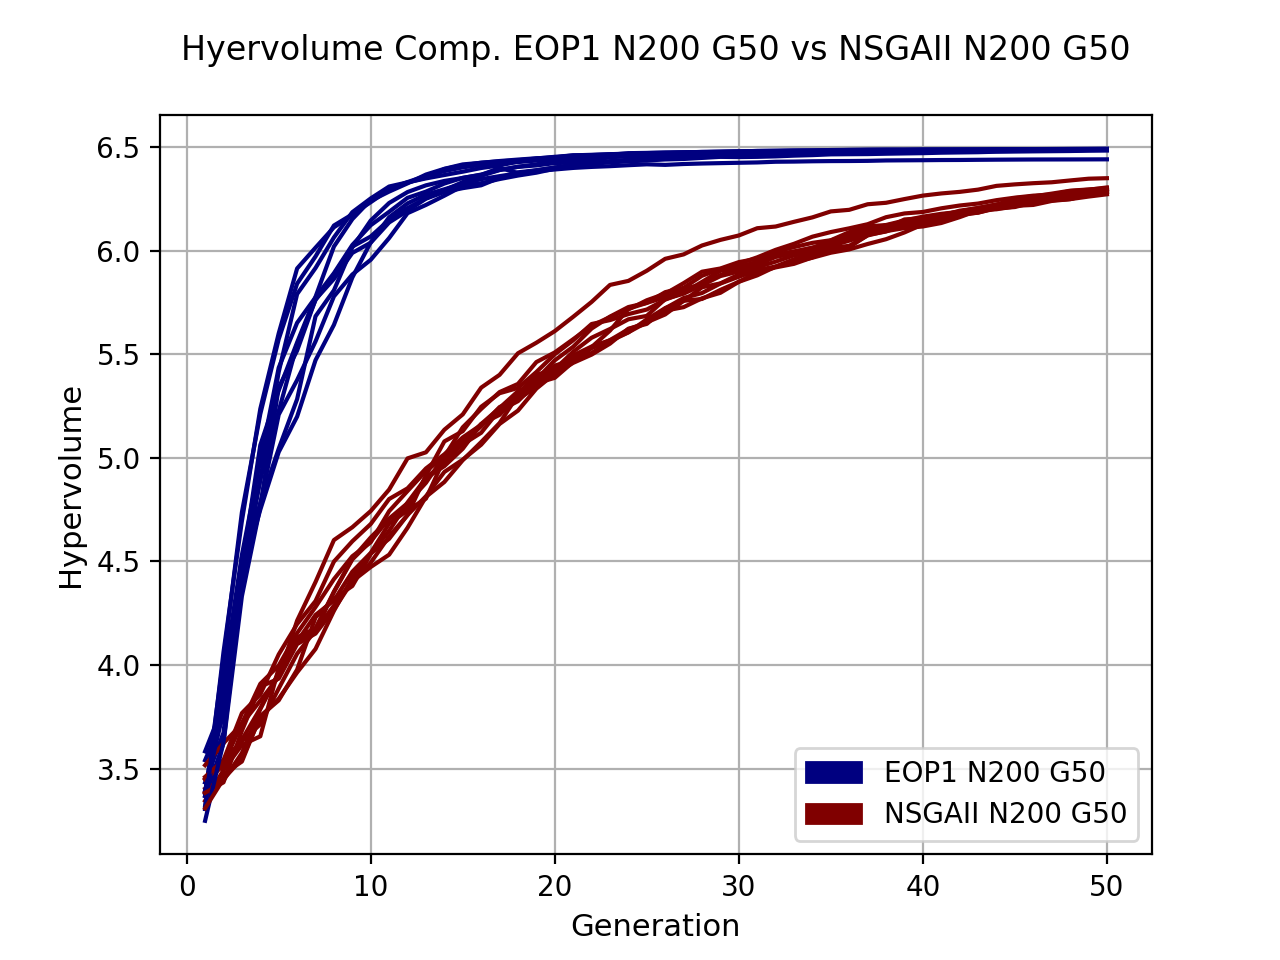
\includegraphics[scale=0.35]{../METRICS_PLOTS/Hypervol_COMP_EOP1N200G50_NSGAIIN200G50.png}
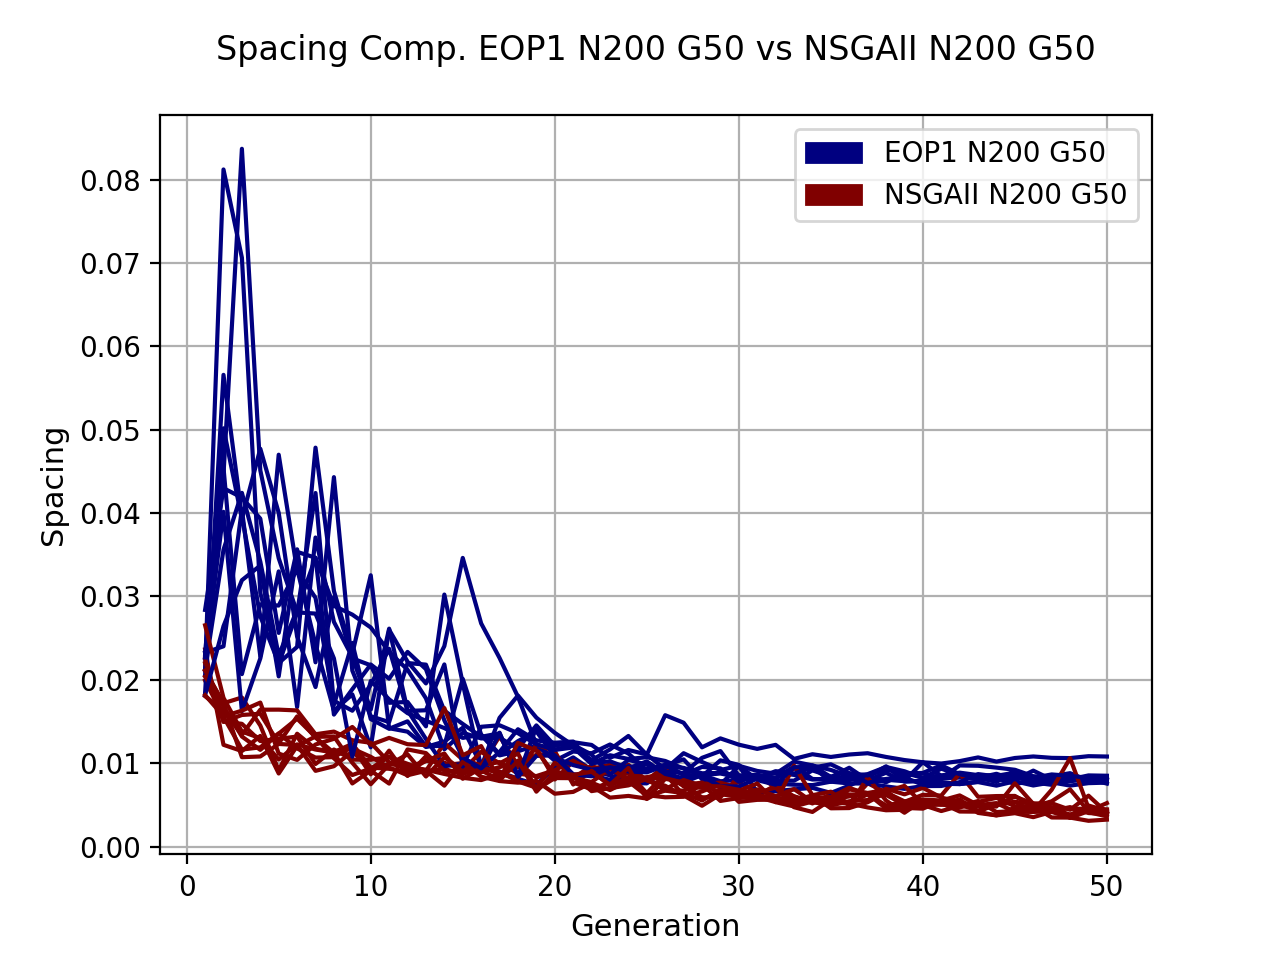
\includegraphics[scale=0.35]{../METRICS_PLOTS/Spacing_COMP_EOP1N200G50_NSGAIIN200G50.png}
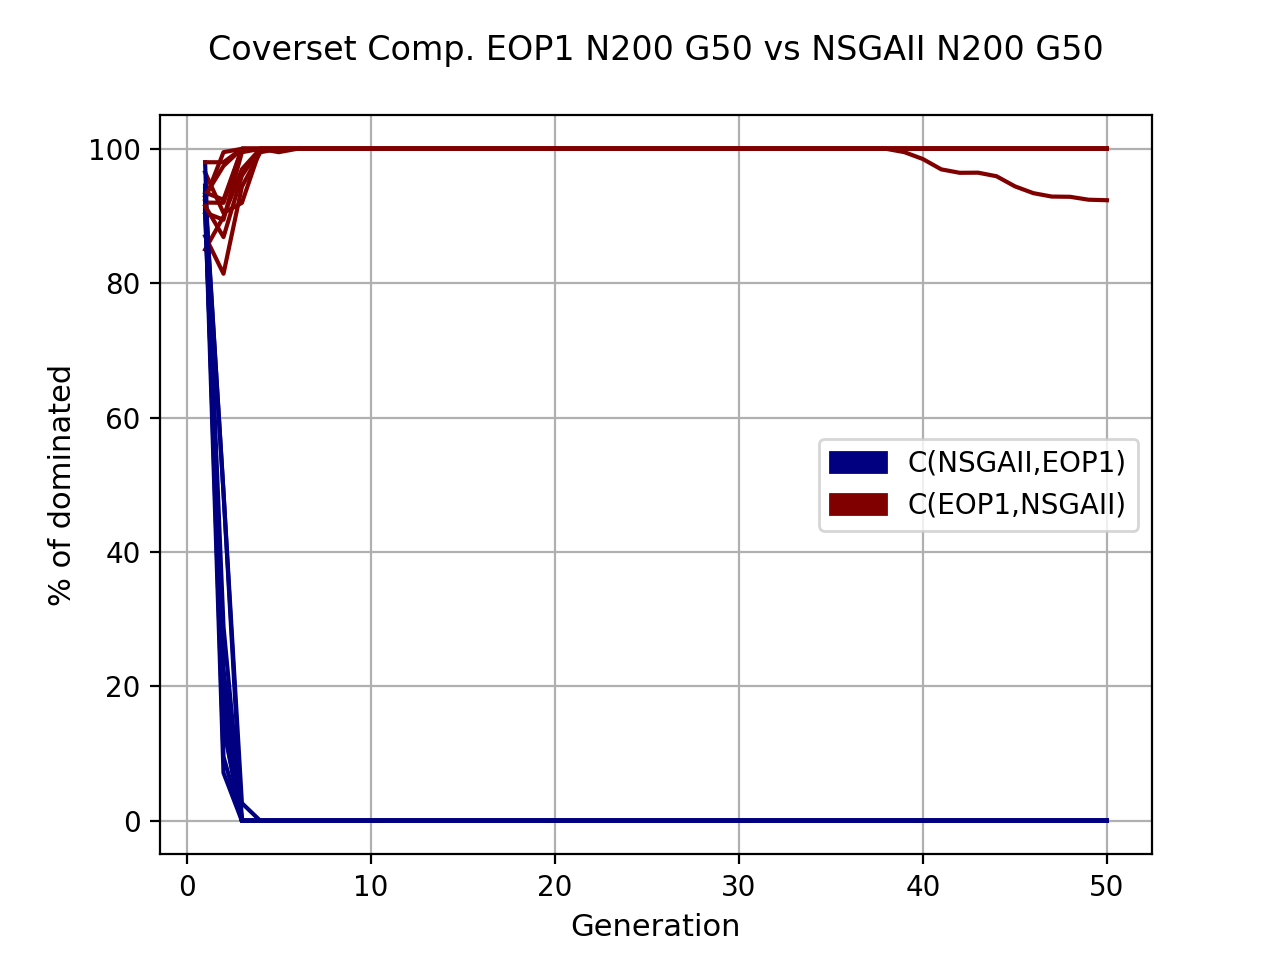
\includegraphics[scale=0.35]{../METRICS_PLOTS/CoverSet_COMP_EOP1N200G50_NSGAIIN200G50.png}\\
\caption{MOEA/D + EOP1. Comparación de métricas con NSGAII para 10000 EV.}
\label{fig:7}
\end{figure}

Aunque en este apartado no hemos realizado (explícitamente) un análisis de las soluciones (población final y NSD) en el último apartado de esta sección presentaremos una comparativa conjunta de las últimas generaciones y de los conjuntos no dominados (NSD) para todos los casos y todos los algoritmos (y operadores).

\noindent\textbf{EXPERIMENTACIÓN PARA 4000 EVALUACIONES}\\

Ya presentamos para 10000 evaluaciones el comportamiento del algoritmo es adecuado, esto es, a través de las generaciones los individuos se aproximan al frente. No vamos a volver a presentarlo para el caso de 4000 evaluaciones, pues sigue lógicamente el mismo esquema (en los apéndices se presentan las gráficas que atestiguan lo expuesto). Por tanto pasaremos directamente a evaluar las métricas y a razonar directamente sobre los resultados obtenidos en dicho análisis.  \\

En la \hyperref[fig:8]{figura 8} se presentan las gráficas del desarrollo del hypervolumen y el espaciado para cada uno de los casos coniderados en las 4000 evaluaciones en contreto $(N=40, G=100)$, $(N=80, G=50)$, $(N=100, G=40)$. Como podemos apreciar el comportamiento es similar a los presentados para las 10000 evaluaciones, denotándose que la convergencia (hipervolumen) se desarrolla de forma análoga a como lo hacía para los casos previos (viendo la forma de la curva, dado que los valores no son comparables debido a la desigualdad del punto de referencia en cada caso), pero truncada a las iteraciones correspondientes (aproximadamente). De igual forma el espaciado disminuye notablemente con el aumento del número de subproblemas, lo que sin duda se adecua a los resultados presentados previamente.\\

Si realizamos una comparativa (al igual que en el caso de 10000 ev) con el algoritmo \textit{NSGAII} obtenemos conclusiones análogas a las ya presentadas previamente, descando que en cuanto a convergencia en todos los casos nuestro algoritmo supera al algoritmo \textit{NSGAII}, en espaciado ocurre al contrario y en cuanto al cover set, para el caso $N=40$ el frente más del 50\%   del frente (final) de \textit{NSGAII} es dominado por el de nuestro algoritmo, mientras que apenas un 5\% del frente de nuestro algoritmo es dominado por el competidor. En los otros dos casos el cover set es mucho más claro de forma que aparentemente (para ambos casos) el 100\% del frente es dominado (en todas las ejecuciones) por el frente final (última generación) de nuestro algoritmo y mientras que para ningún punto (o desde luego menor al 1\% o 2\%) se da el comportamiento contrario.\\

De todo ello destacamos la bondad de nuestro algoritmo en cuanto a la convergencia, no tanto para el espaciado (sobre todo si consideramos la última generación, si consideramos el frente NSD veremos que el espaciado mejora notablemente, presentado en la comparativa final de la \hyperref[table:1]{tabla 1}) y en cuanto al cover set, con el número adecuado de subproblemas (mejor que de generaciones) nuestro algoritmo domina practicamente en su totalidad a \textit{NSGAII}. \\

\begin{center}
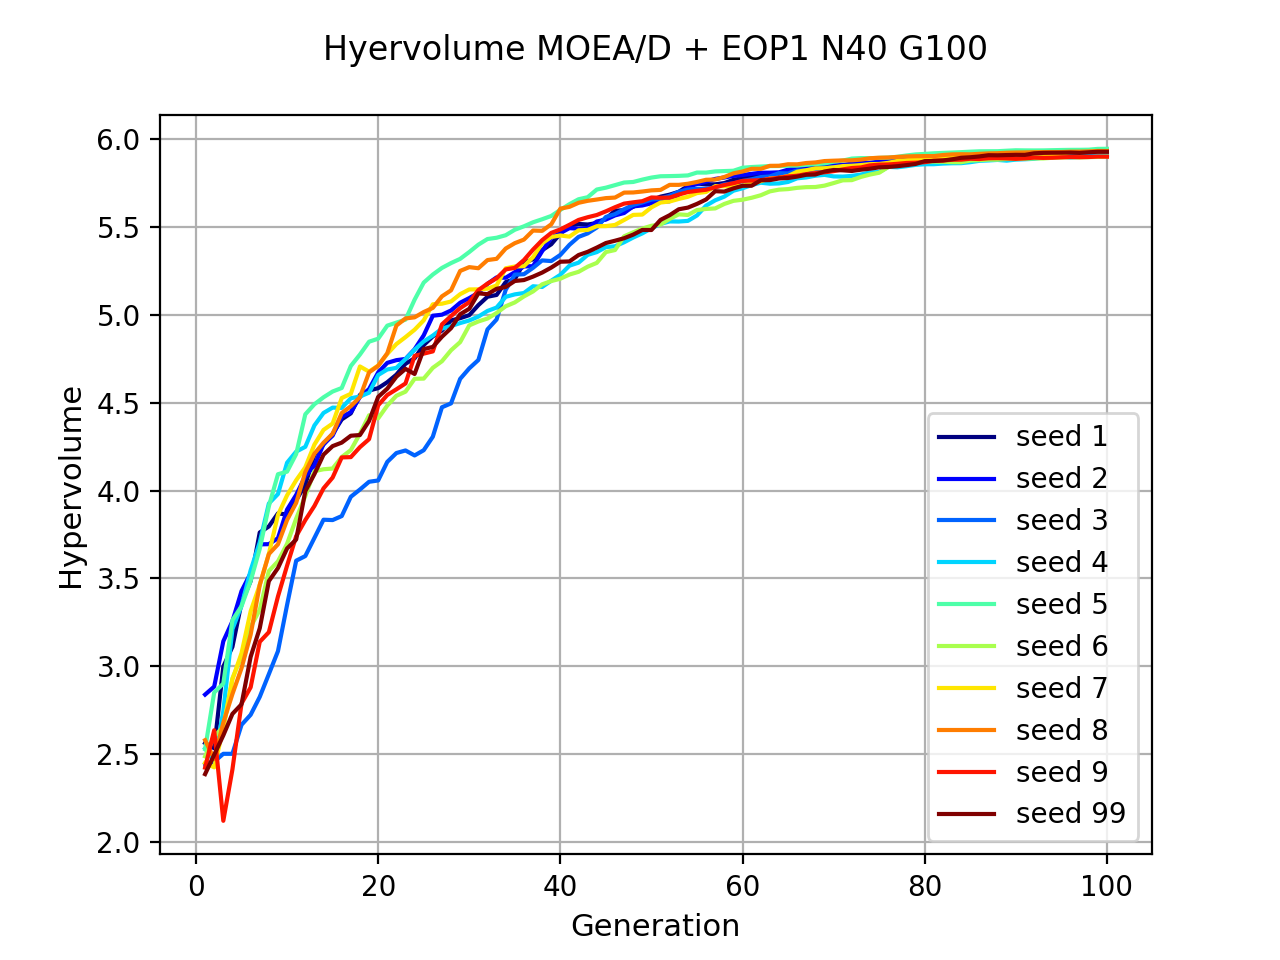
\includegraphics[scale=0.43]{figures/METRICS_EOP1/Hypervol_N40_G100.png} \quad 
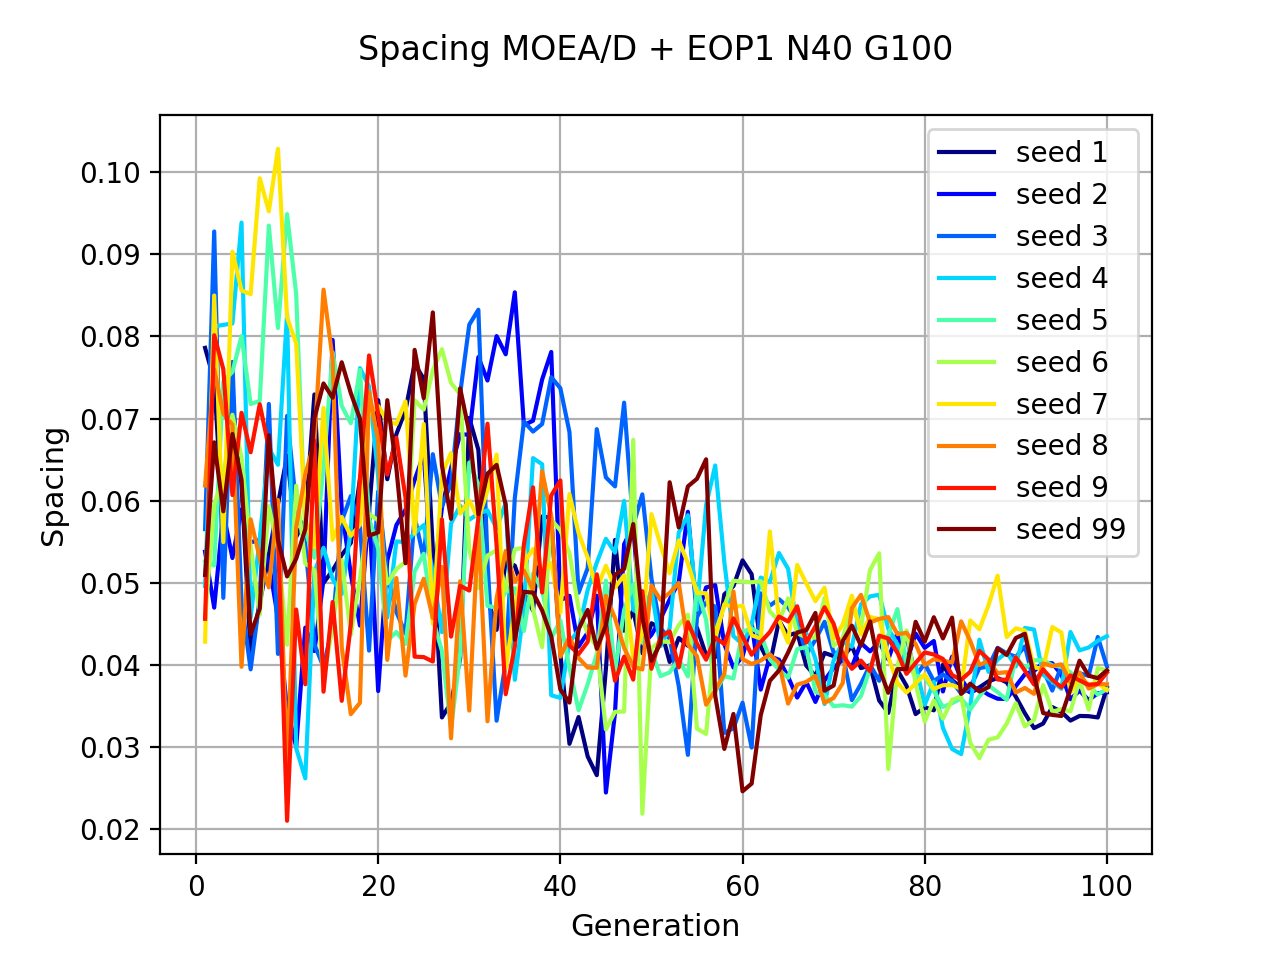
\includegraphics[scale=0.43]{figures/METRICS_EOP1/Spacing_N40_G100.png}\\
\end{center}

\begin{figure}[H]
\centering
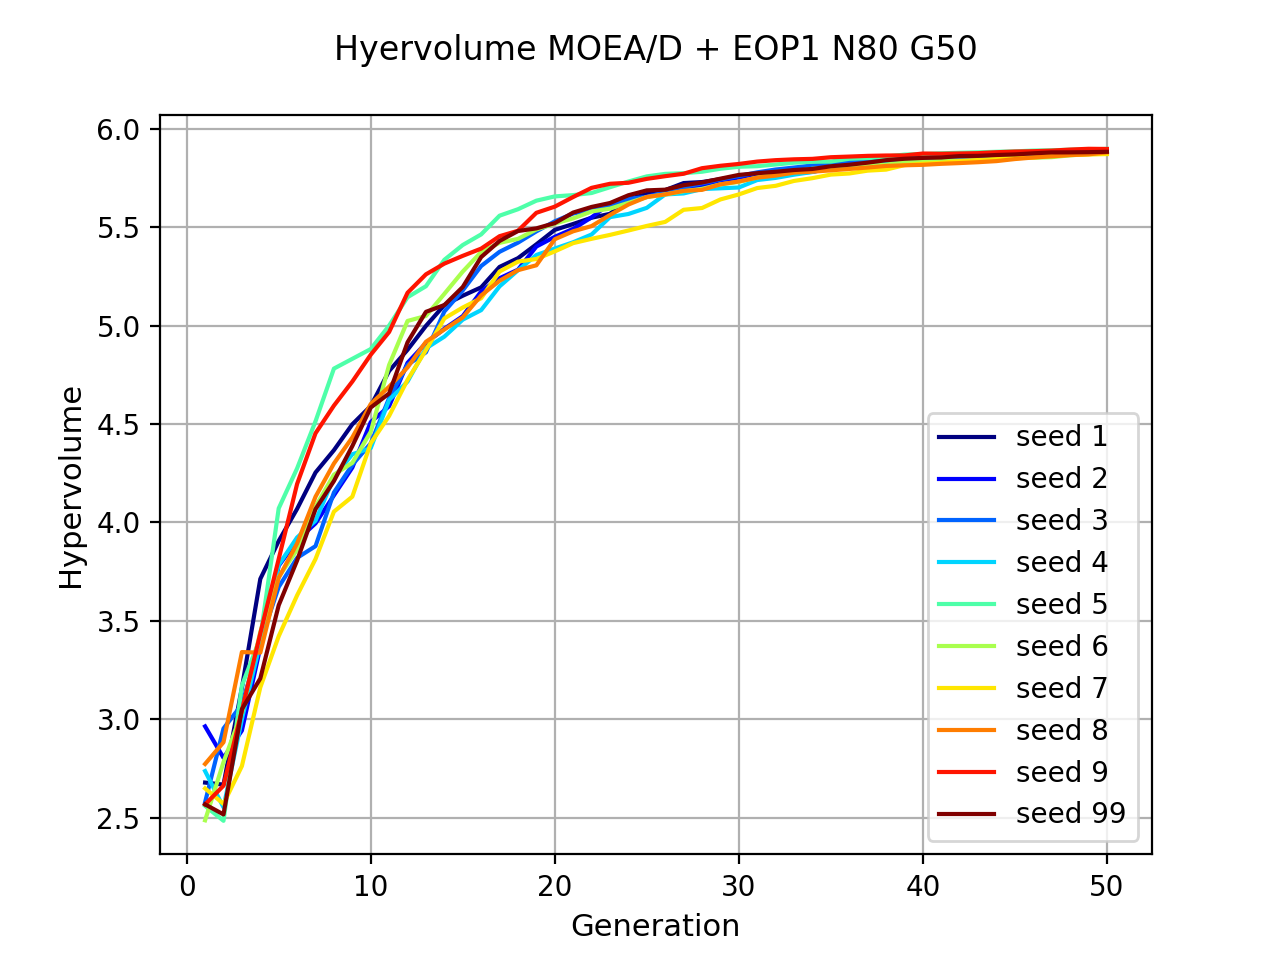
\includegraphics[scale=0.43]{figures/METRICS_EOP1/Hypervol_N80_G50.png}\quad 
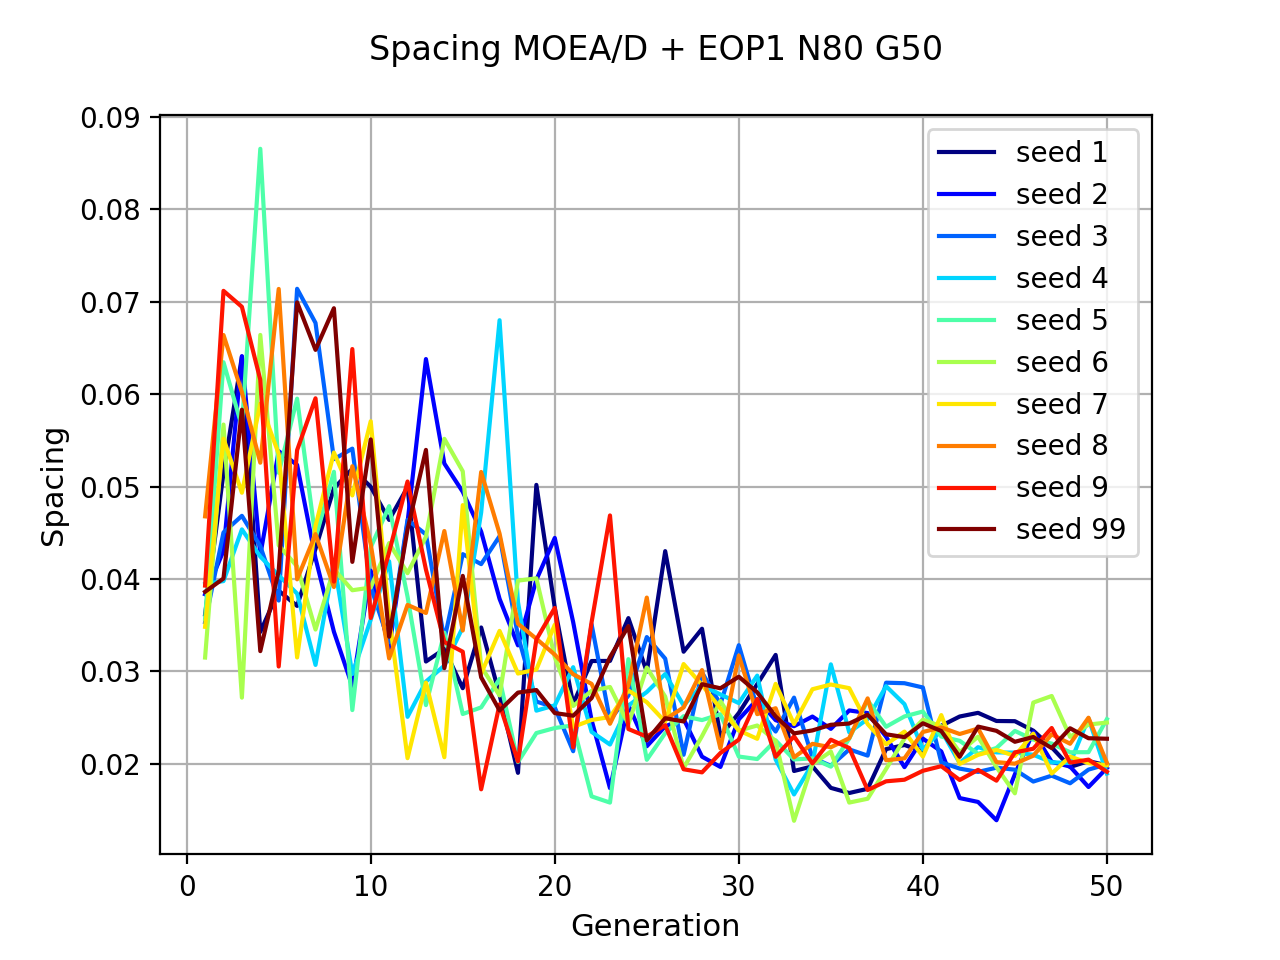
\includegraphics[scale=0.43]{figures/METRICS_EOP1/Spacing_N80_G50.png}\\
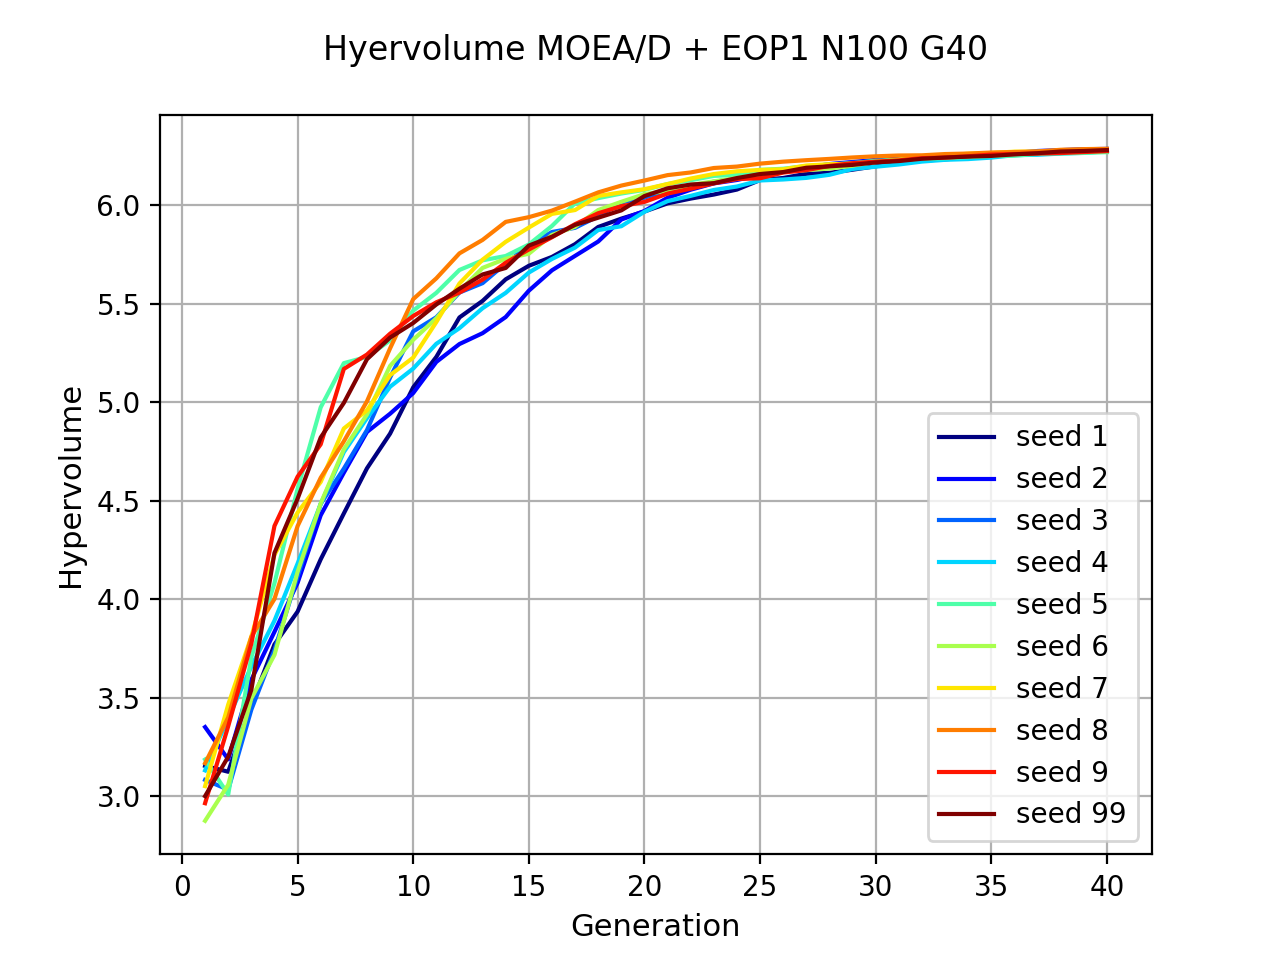
\includegraphics[scale=0.43]{figures/METRICS_EOP1/Hypervol_N100_G40.png}\quad 
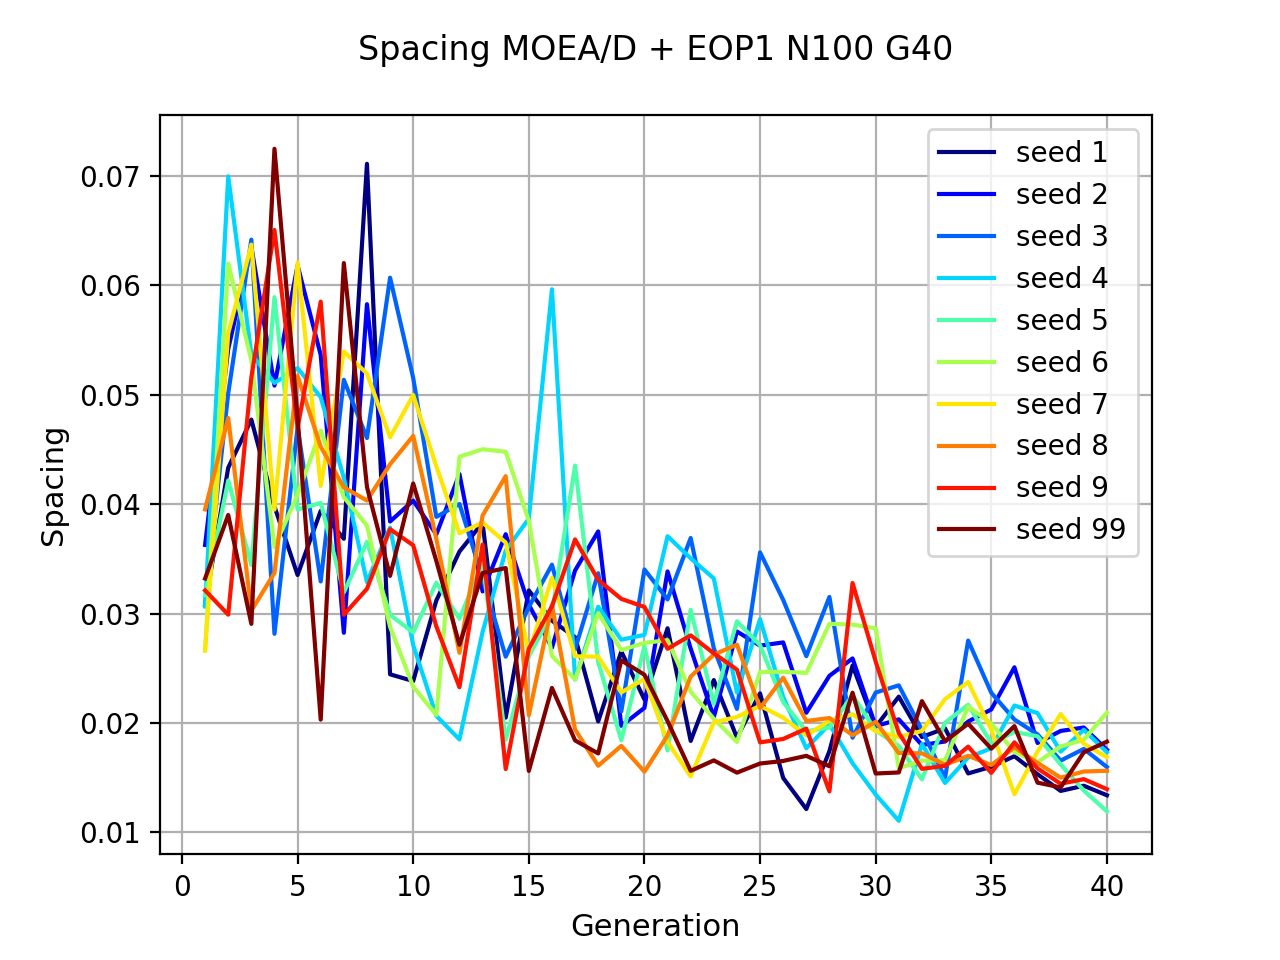
\includegraphics[scale=0.43]{figures/METRICS_EOP1/Spacing_N100_G40.png}\\
\caption{MOEA/D + EOP1. Métricas para 4000EV}
\label{fig:8}
\end{figure}

\hfill\break

\begin{center}
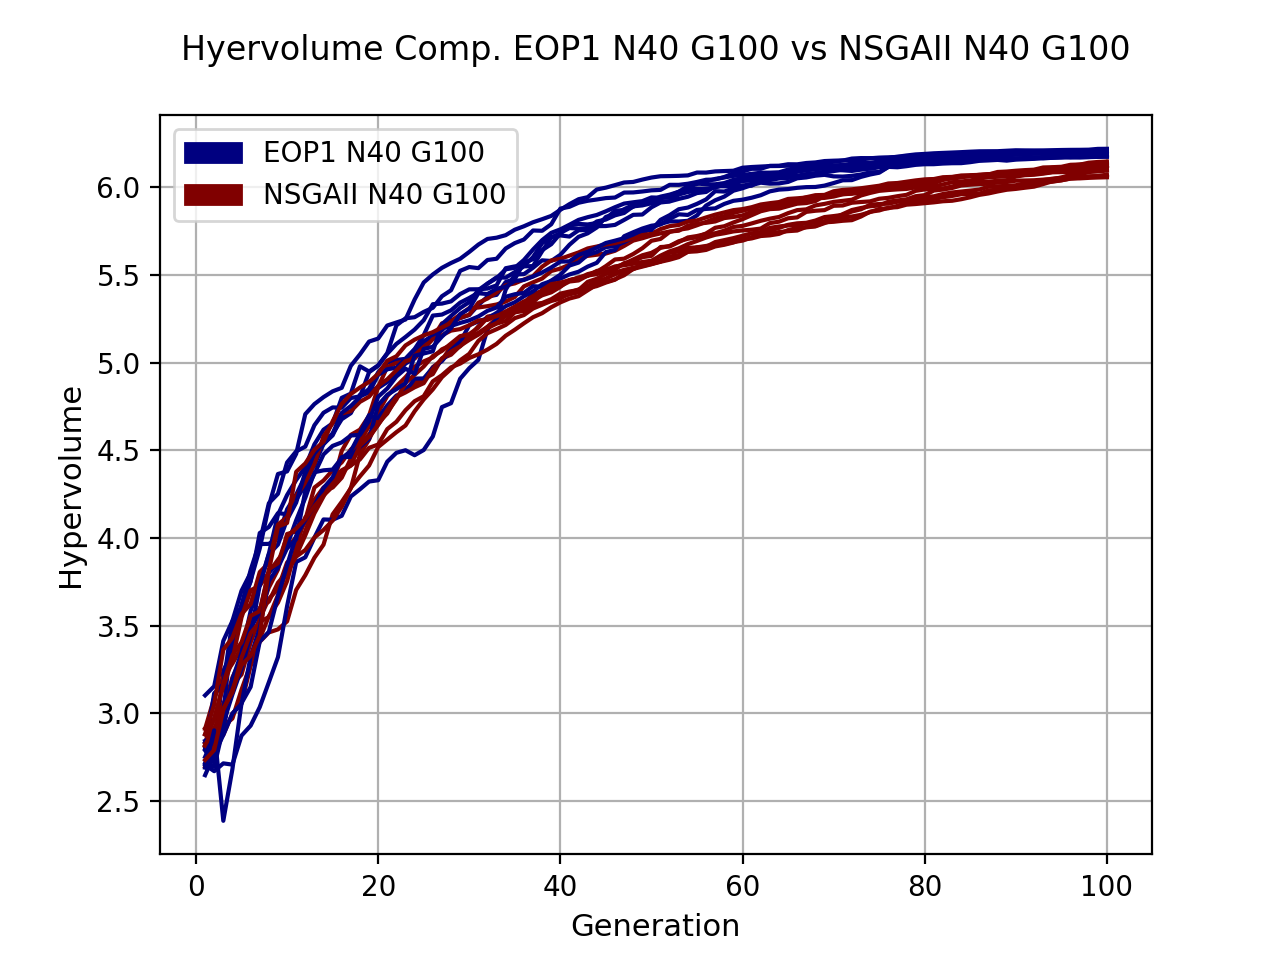
\includegraphics[scale=0.35]{../METRICS_PLOTS/Hypervol_COMP_EOP1N40G100_NSGAIIN40G100.png}
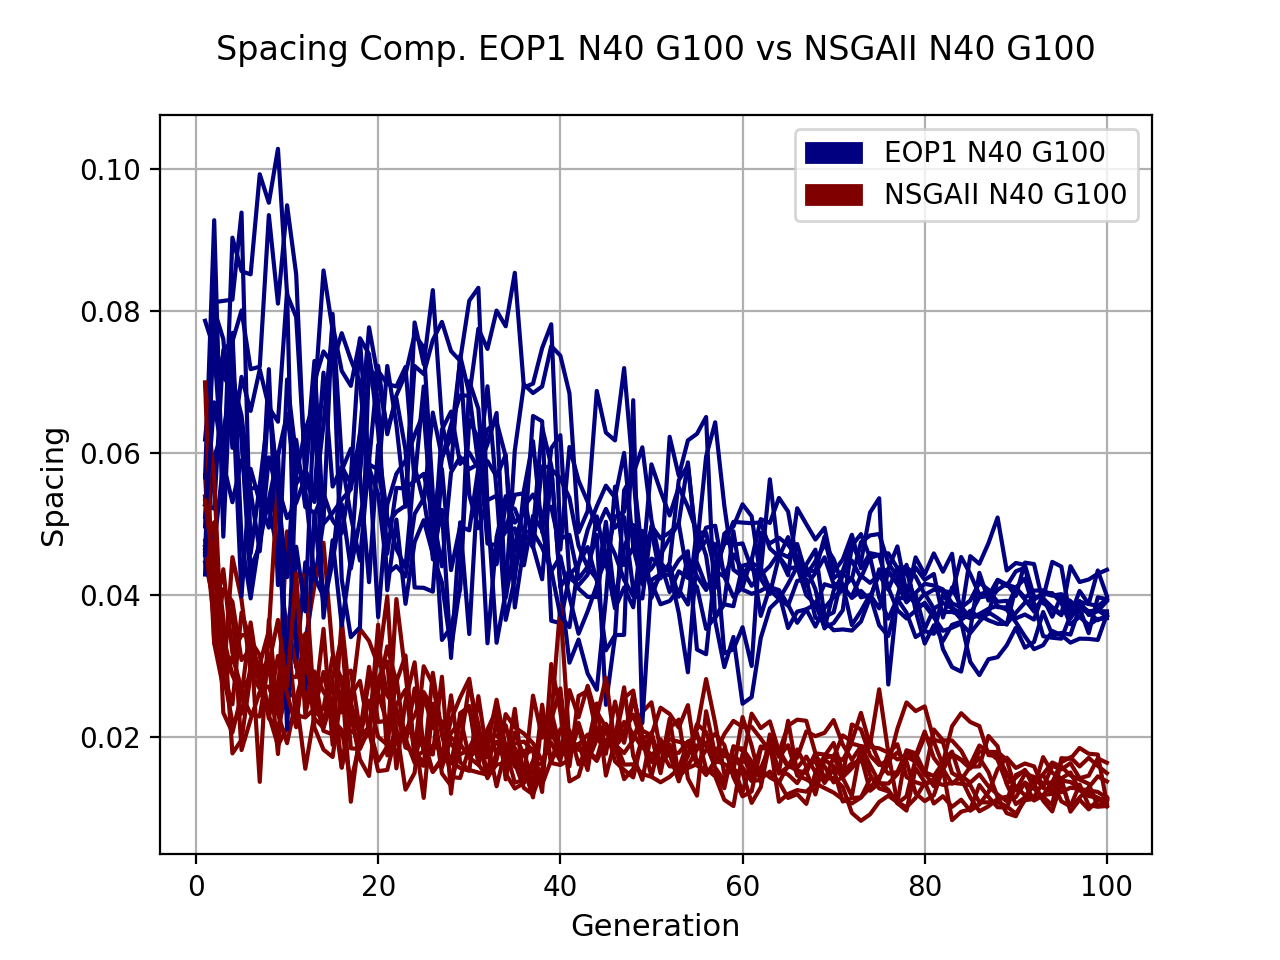
\includegraphics[scale=0.35]{../METRICS_PLOTS/Spacing_COMP_EOP1N40G100_NSGAIIN40G100.png}
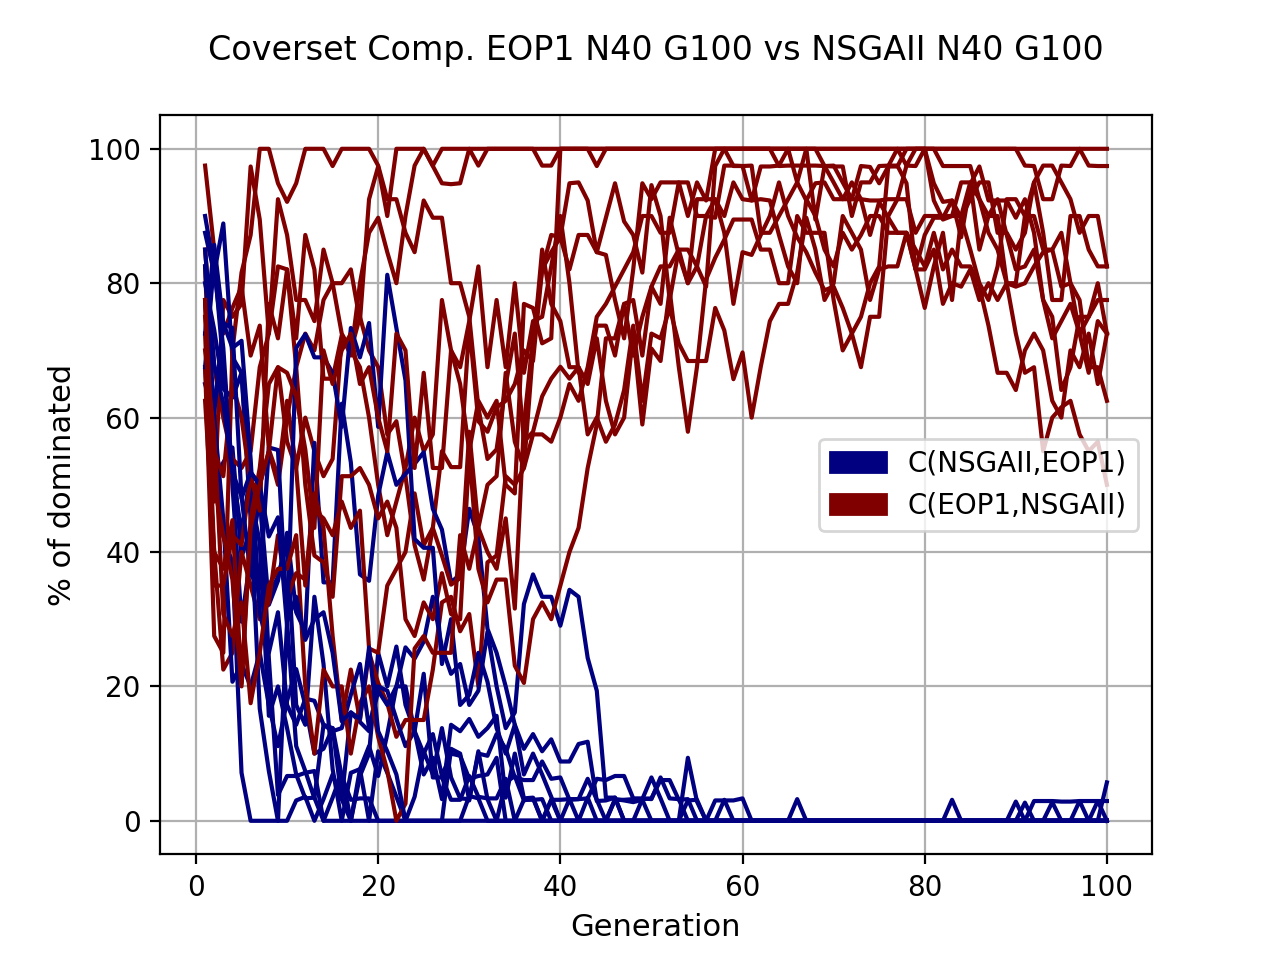
\includegraphics[scale=0.35]{../METRICS_PLOTS/CoverSet_COMP_EOP1N40G100_NSGAIIN40G100.png}\\
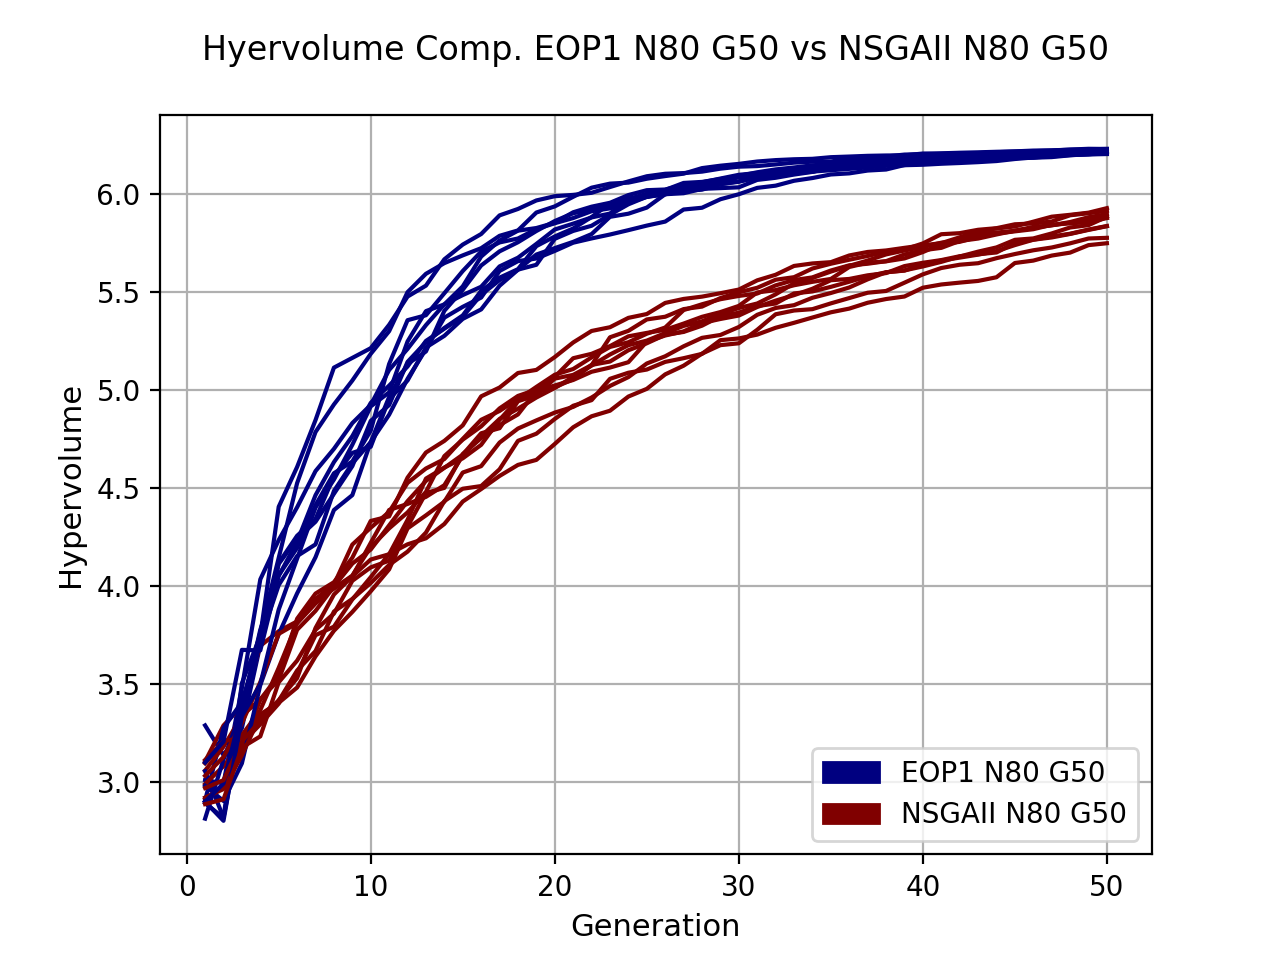
\includegraphics[scale=0.35]{../METRICS_PLOTS/Hypervol_COMP_EOP1N80G50_NSGAIIN80G50.png}
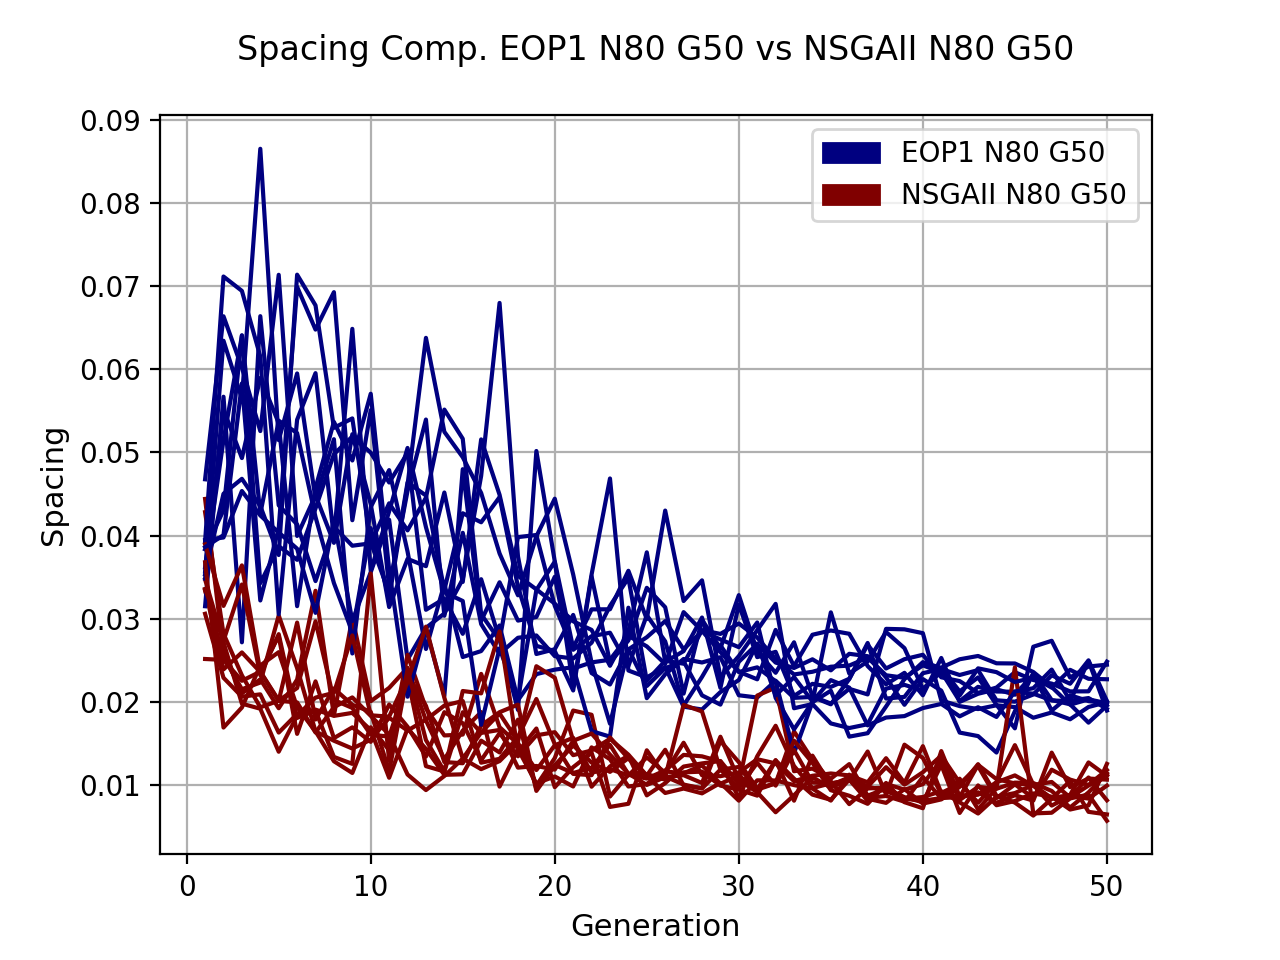
\includegraphics[scale=0.35]{../METRICS_PLOTS/Spacing_COMP_EOP1N80G50_NSGAIIN80G50.png}
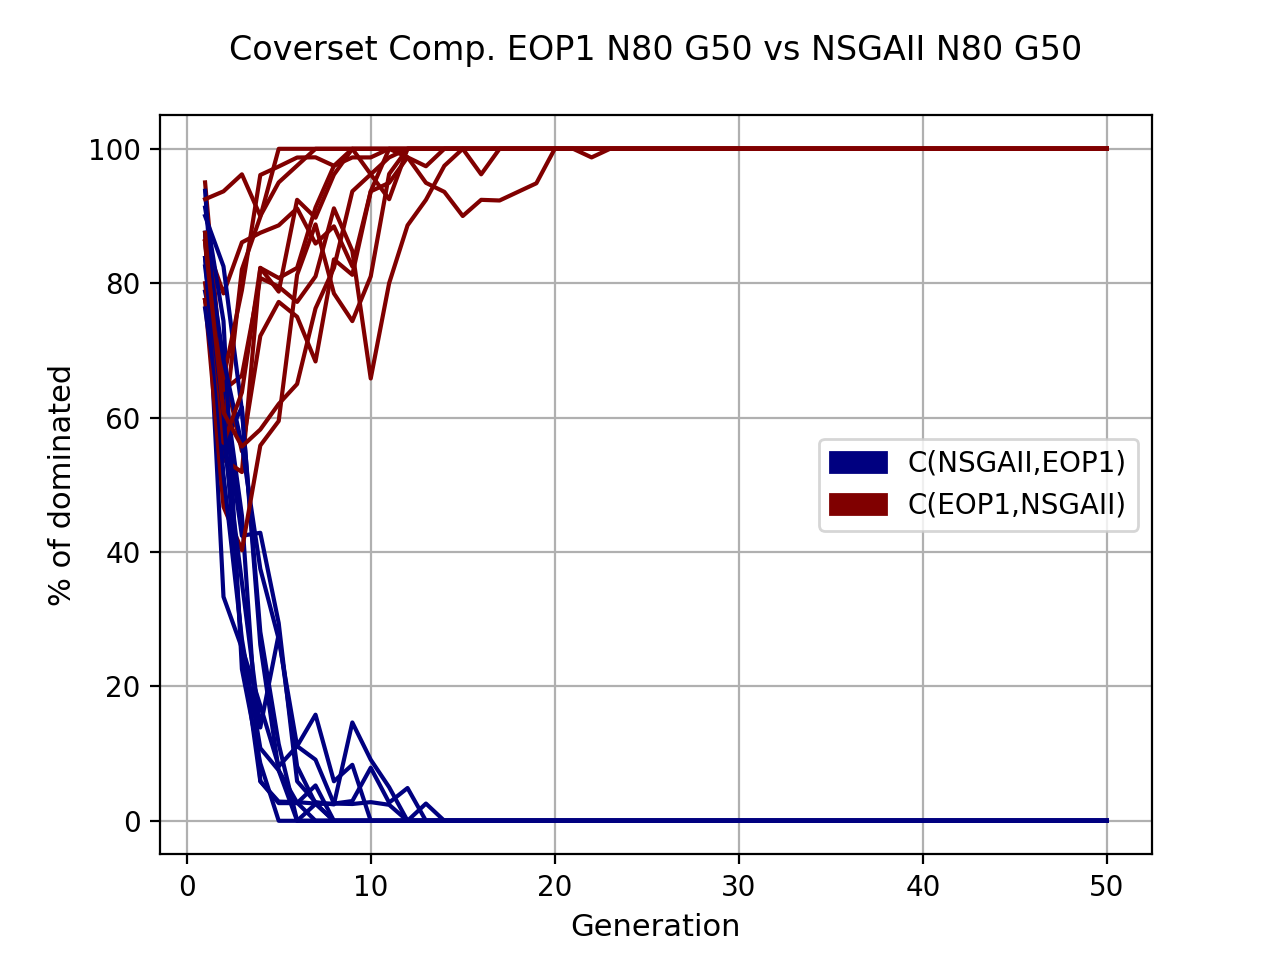
\includegraphics[scale=0.35]{../METRICS_PLOTS/CoverSet_COMP_EOP1N80G50_NSGAIIN80G50.png}\\
\end{center}

\begin{figure}[H]
\centering
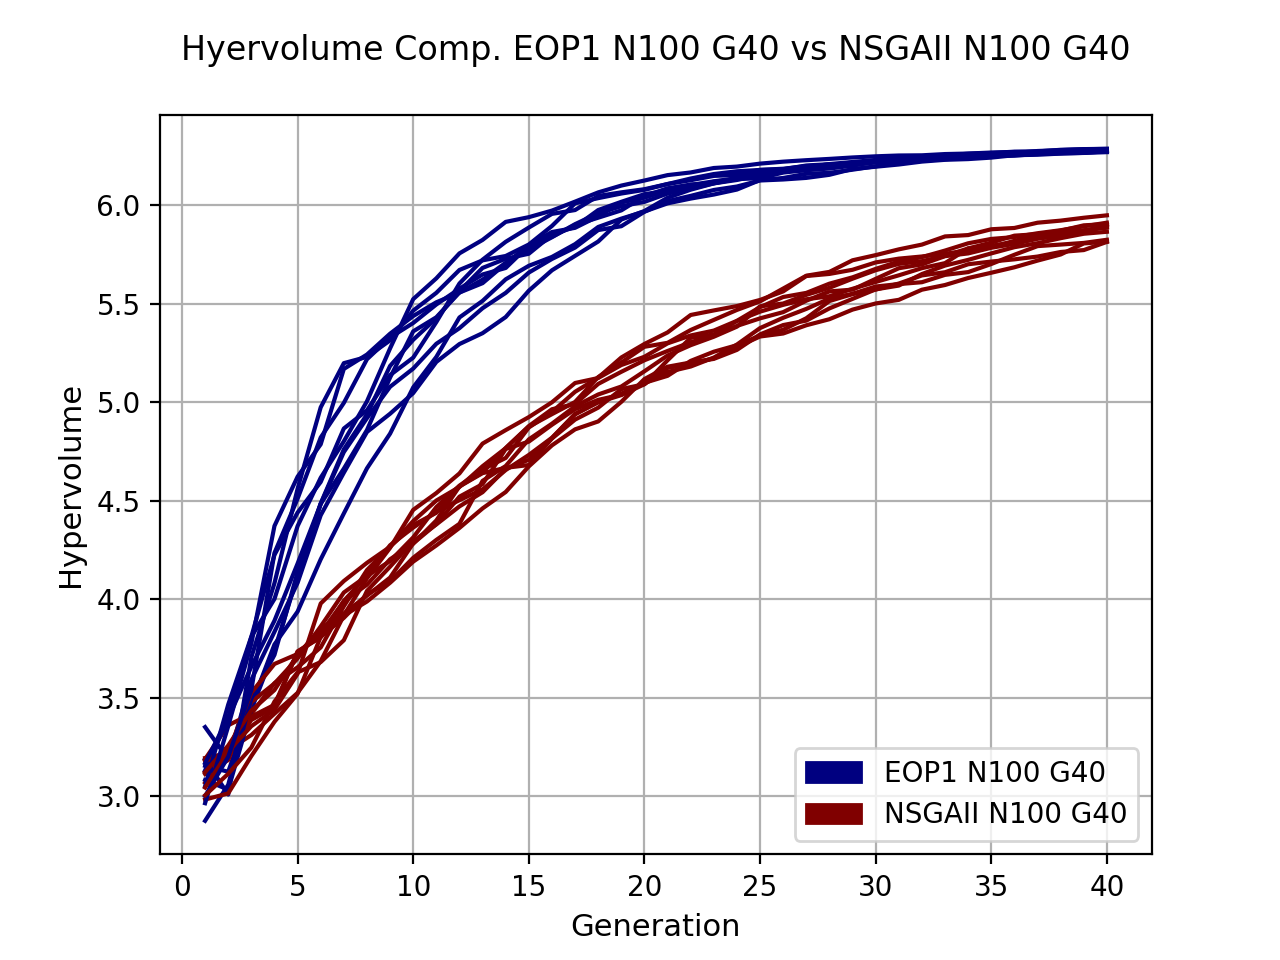
\includegraphics[scale=0.35]{../METRICS_PLOTS/Hypervol_COMP_EOP1N100G40_NSGAIIN100G40.png}
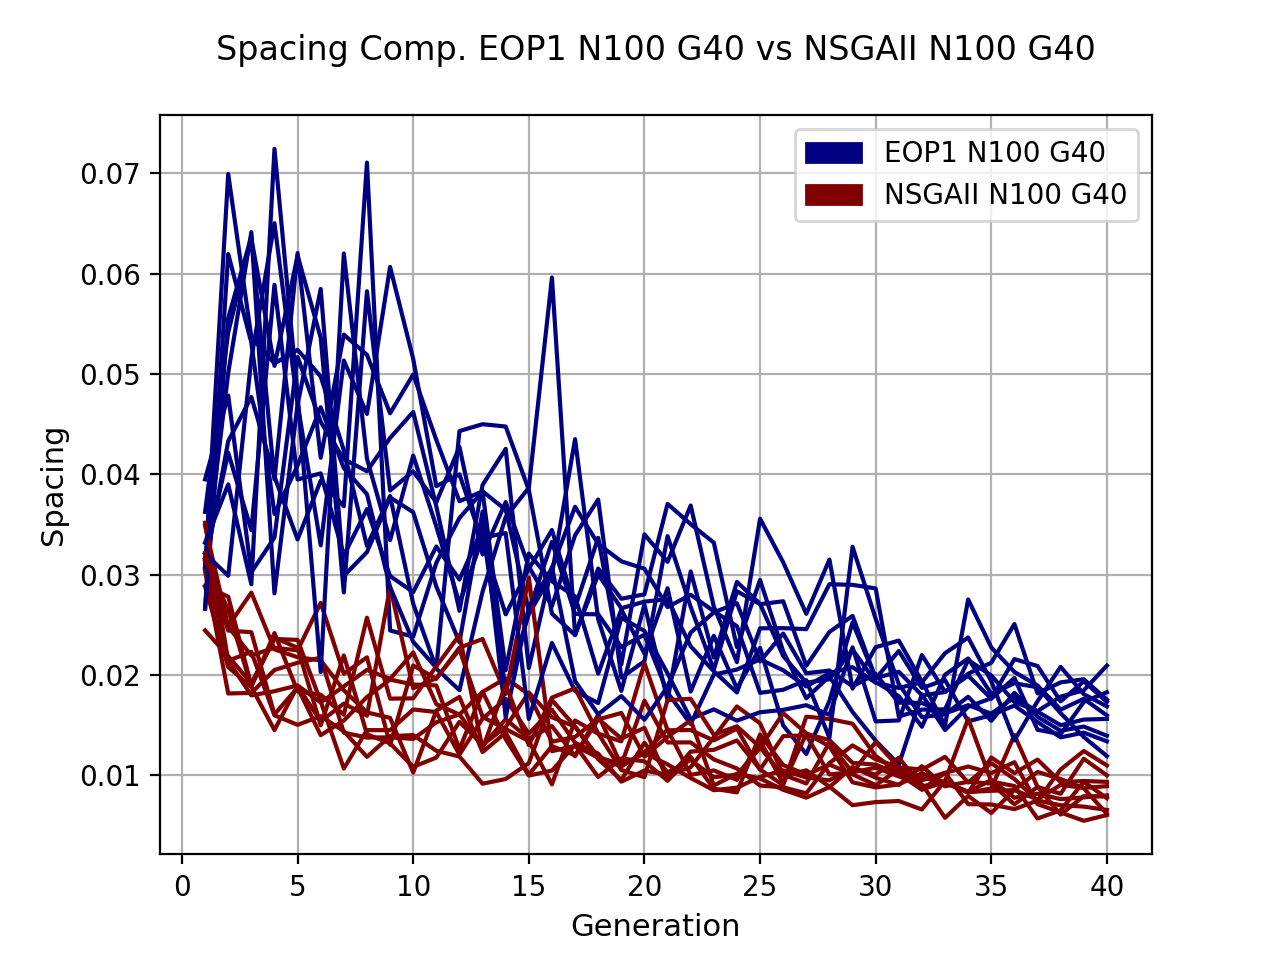
\includegraphics[scale=0.35]{../METRICS_PLOTS/Spacing_COMP_EOP1N100G40_NSGAIIN100G40.png}
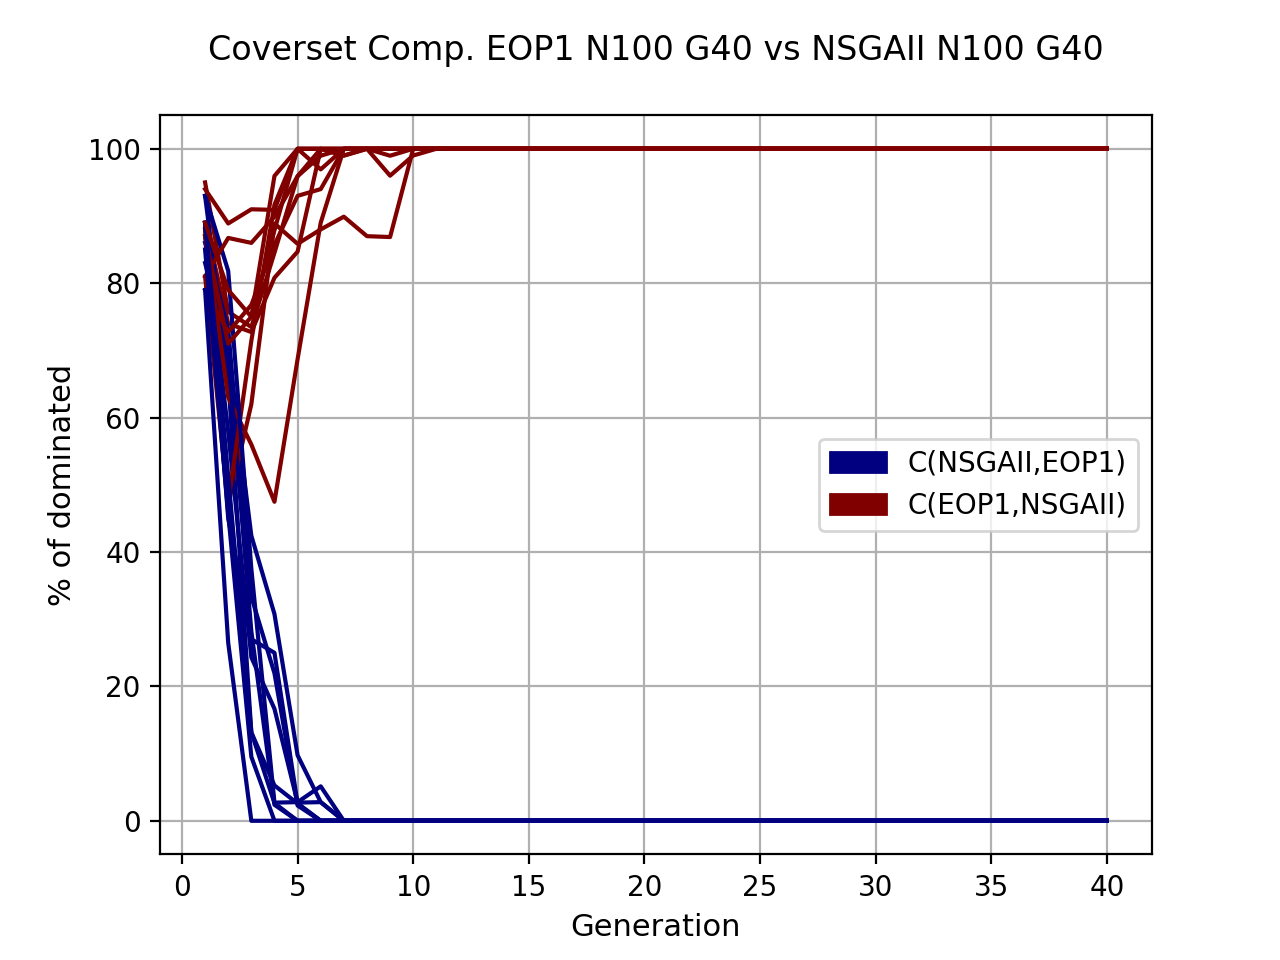
\includegraphics[scale=0.35]{../METRICS_PLOTS/CoverSet_COMP_EOP1N100G40_NSGAIIN100G40.png}\\
\caption{MOEA/D + EOP1. Comparación de métricas con NSGAII para 4000 EV.}
\label{fig:9}
\end{figure}





\subsection{Evaluación MOEA/D + EOP2 con ZDT3}

De igual manera a lo presentado para EOP1 vamos a realizar algunas pruebas para comprobar la efectividad del algoritmo con EOP2. Tanto utilizando una capacidad de cómputo de $10000$ evaluaciones como una de $4000$ evaluaciones (con los mismos repartos ya presentados).\\

\justify
\subsubsection{Experimentación con 1OOOO ev.}

En la \hyperref[fig:10]{\textit{figura 10}} presentamos tres gráficos pertenecientes a una ejecución característica del algoritmo con el operador evolutivo EOP3, $N=100, G=100$ y $T=15$ (para todos los casos se ha tomado un $15\%$  (recuérdese que en los anexos se muestran varias ejecuciones que validan las discusiones) el primer diagrama muestra el desarrollo de las soluciones en el espacio de objetivos a lo largo de la ejecución del algoritmo (en las distintas generaciones). En él podemos apreciar que, tal como esperábamos a medida que el algoritmo avanza (pasan las generaciones) las soluciones tinden a ir convergiendo hacia el frente real de Pareto (señalado en gris), sin embargo sí podemos notar que dicha convergencia es (generalmente) más lenta que en el caso anterior, aunque parecen alcanzarse buenos valores en la mayoría de las ejecuciones, aunque alguna no haga (ver \textit{s1} en los anexos). Otro aspecto a destacar es la diversidad, en los algoritmos evolutivos es corriente que las soluciones tiendan a concentrarse (se pierde diversidad); en este caso podemos ver dicha tendencia pero al mismo tiempo se puede notar que se tiende a conservar cierta dispersión en los puntos lo que denota una intención de mantener la diversidad (objetivo de todo algoritmo evolutivo).\\

En el segundo diagrama se presenta el conjunto de las soluciones no dominadas calculadas por el algoritmo, que parece estar bastante próximo al frente real de Pareto, tanto en proximidad (convergencia) como en cobertura (dispersión) en los puntos del frente. Lo que denota, a priori, y a falta de métricas un buen comportamiento del algoritmo. De hecho, esos puntos podrían ser considerados como la salida del algoritmo, esto es la aproximación al frente de Pareto que parece ser relativamente fiel al frente real (mostrado en gris).\\

Finalmente, presentamos una gráfica comparativa para nuestro algoritmo y para el algoritmo \textit{NSGA-II}. Para ello hemos representado las soluciones en el espacio de objetivos, las cuales corresponden a la última generación de ejecuciones en iguales condiciones $(G=100, N=100)$ para ambos algoritmos. Podemos ver que en cuanto a convergencia (proximidad al frente real) el frente del nuestro algoritmo es sensiblemente mejor que el frente proporcionado por  \textit{NSGA-II} (una mayoría de los puntos rojos están por debajo de los azules), mientras que en dispersión parece que los puntos del frente de \textit{NSGA-II} se distribuyen más uniformemente que los de nuestro algoritmo. Pero nótese que si consideramos como salida la proporcionada por el frente de las soluciones no dominadas tanto la cobertura como la convergencia parecen aceptables.\\

\begin{minipage}[H]{\linewidth}
\begin{minipage}[b]{0.3\linewidth}

\begin{figure}[H]
        \centering
        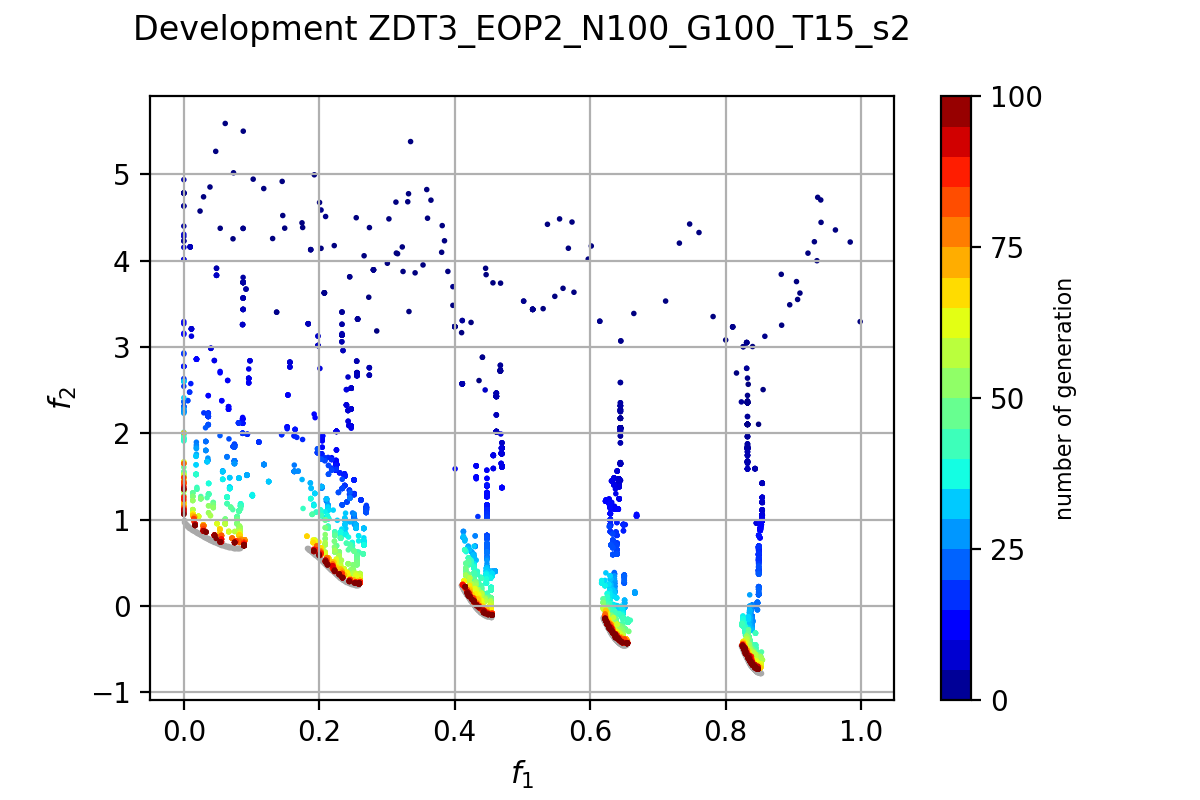
\includegraphics[scale=0.4]{figures/ZDT3_EOP2_N100_G100_T15/s2_dev.png}\\
        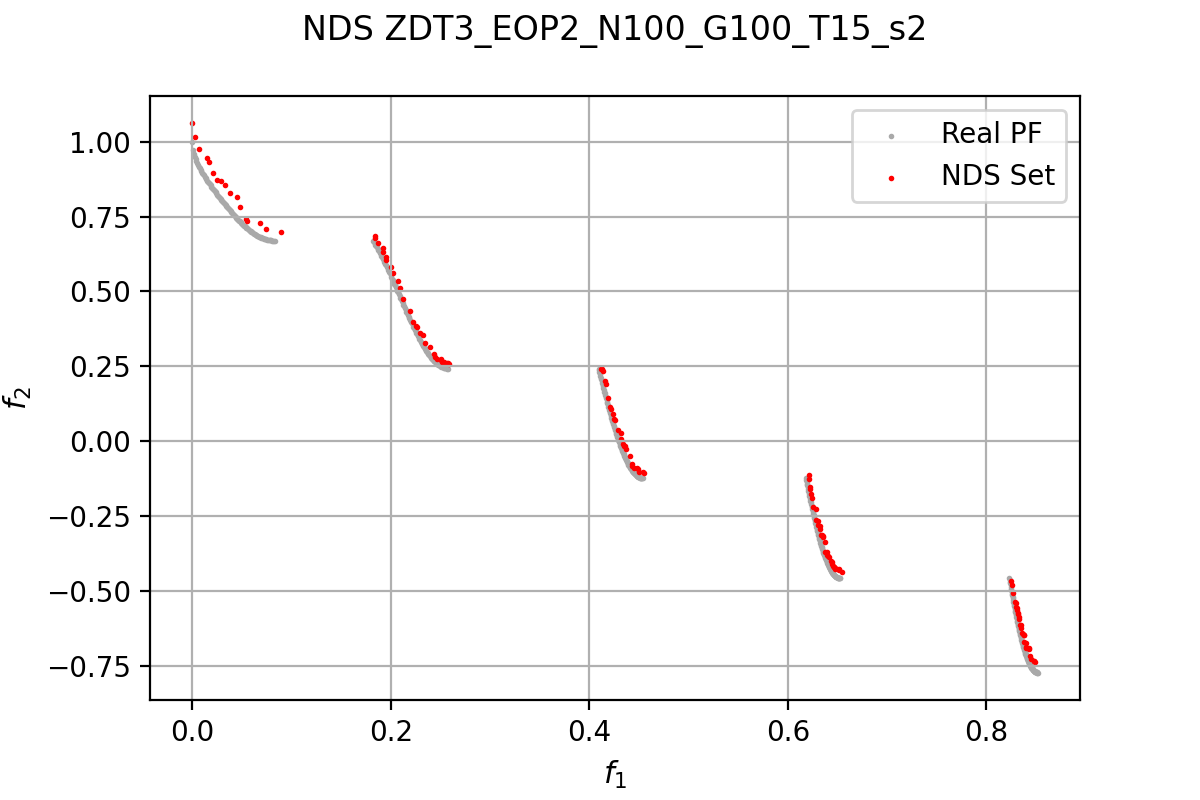
\includegraphics[scale=0.36]{figures/ZDT3_EOP2_N100_G100_T15/s2_nds.png}\\
        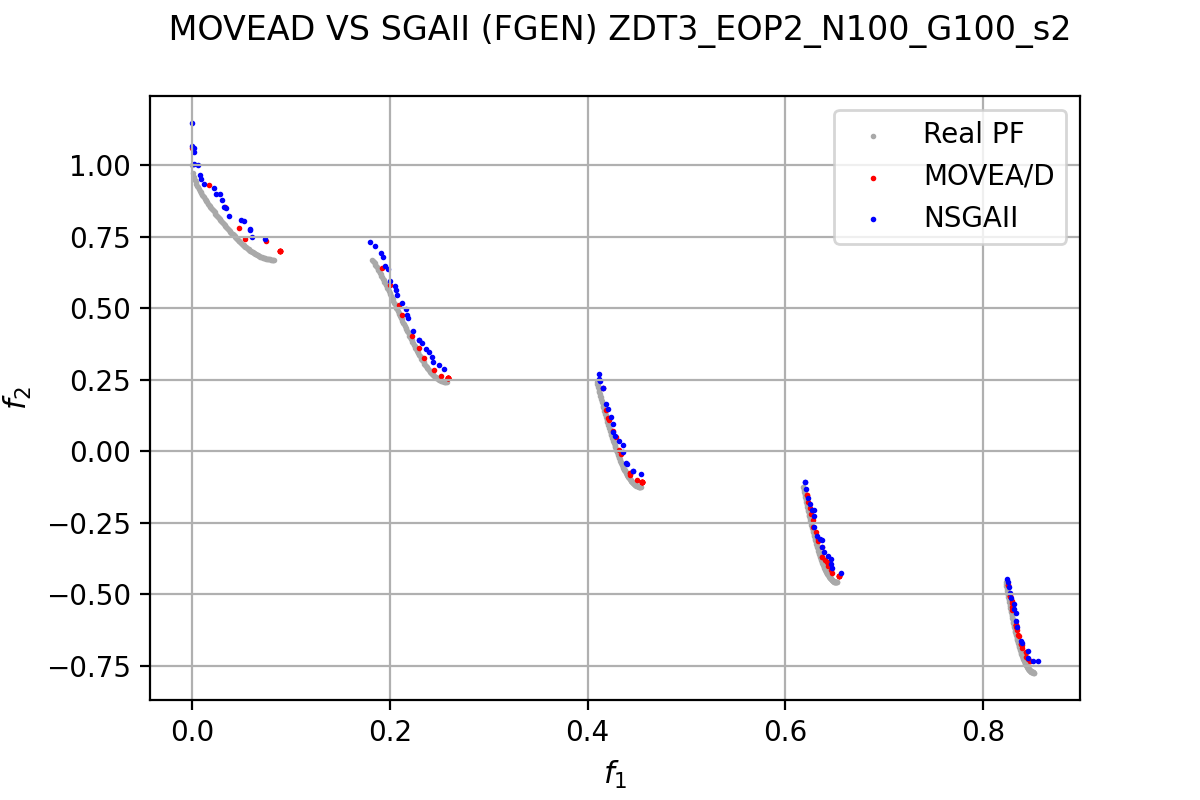
\includegraphics[scale=0.36]{figures/ZDT3_EOP2_N100_G100_T15/s2_comp.png}\\
        \caption{\centering MOEA/D + EOP2 (N100G100)}
        \label{fig:10}
    \end{figure}
\end{minipage} \quad
\begin{minipage}[b]{0.3\linewidth}
\begin{figure}[H]
        \centering
        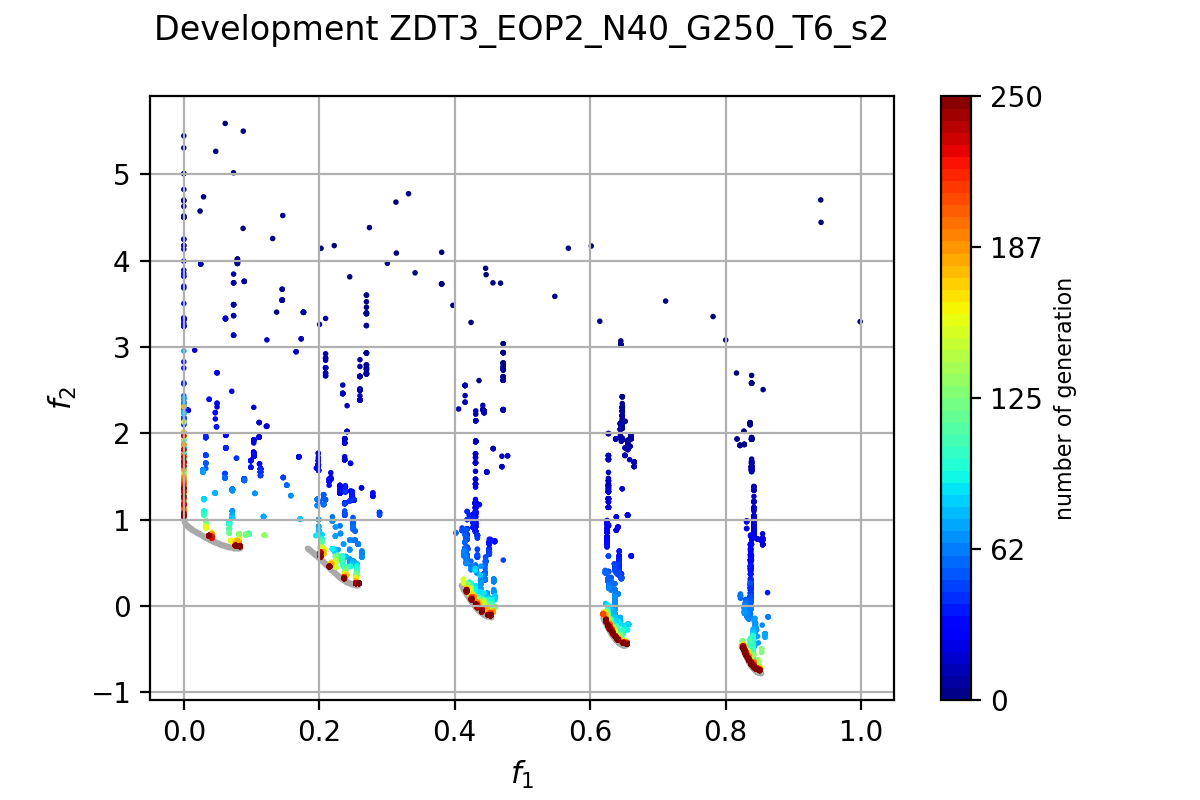
\includegraphics[scale=0.4]{figures/ZDT3_EOP2_N40_G250_T6/s2_dev.png}\\
        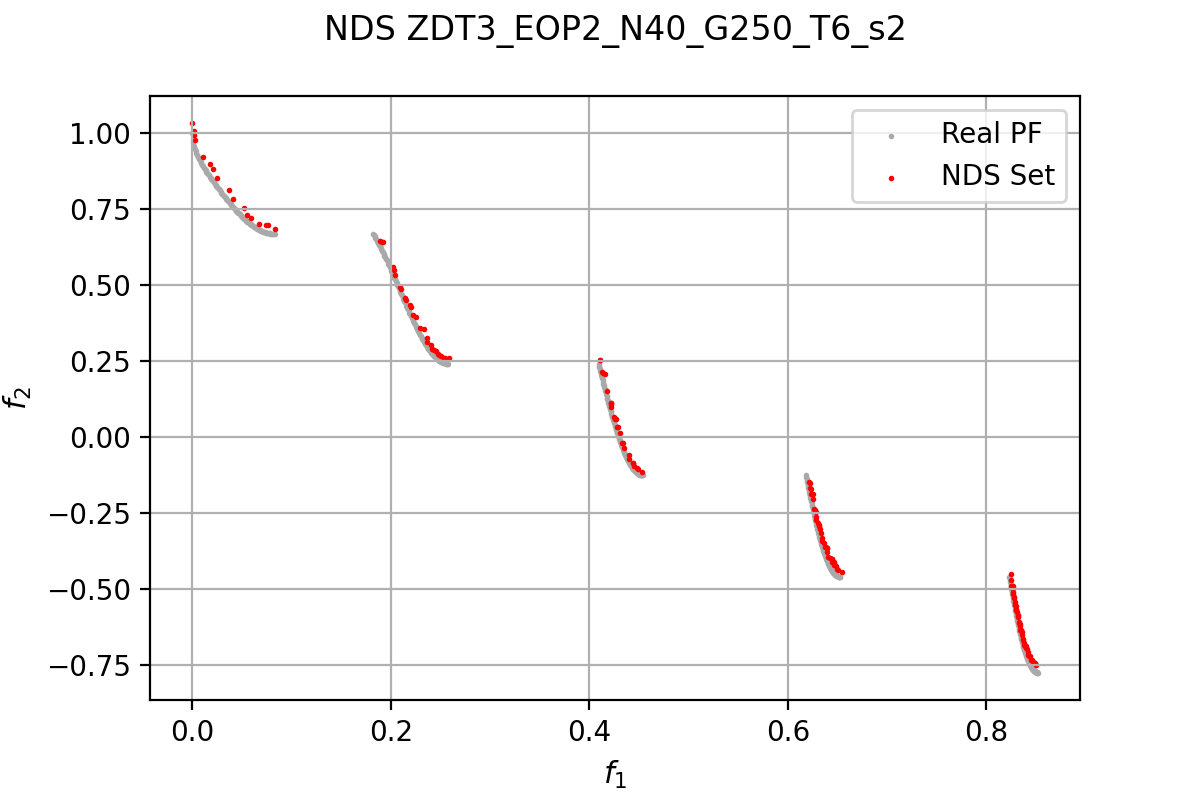
\includegraphics[scale=0.36]{figures/ZDT3_EOP2_N40_G250_T6/s2_nds.png}\\
        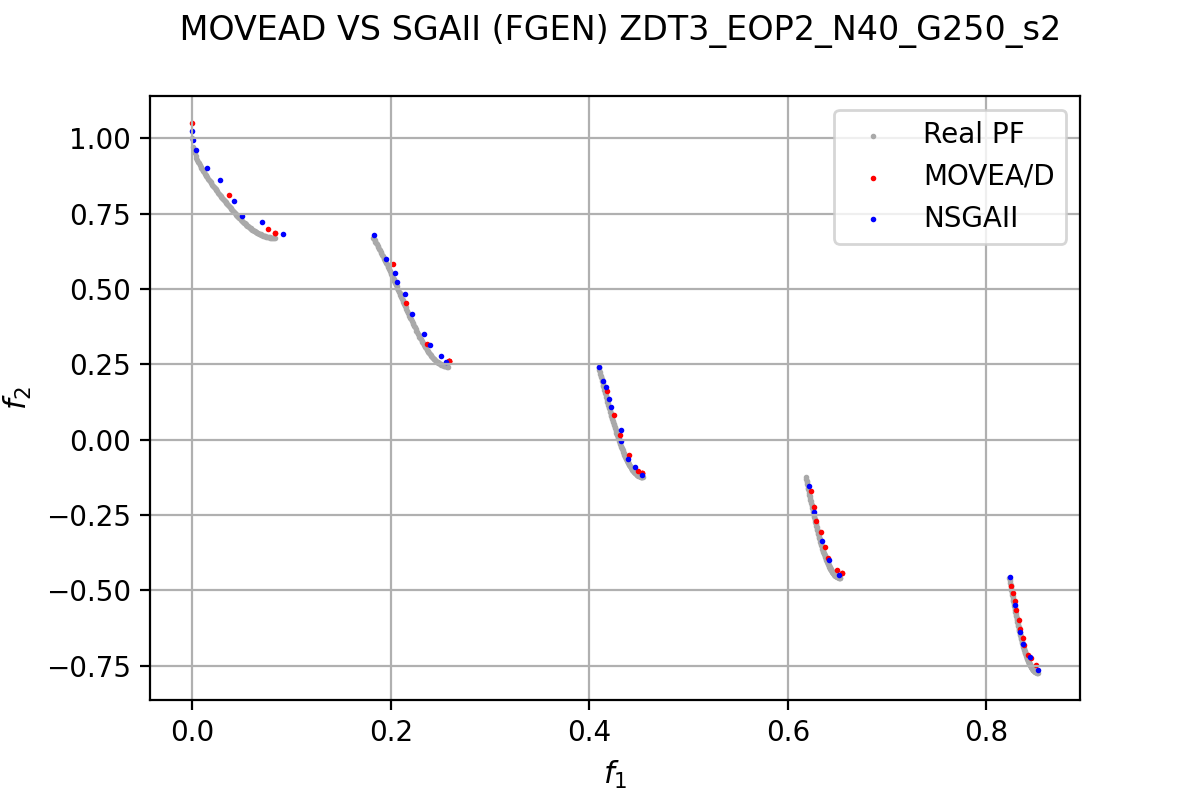
\includegraphics[scale=0.36]{figures/ZDT3_EOP2_N40_G250_T6/s2_comp.png}\\
        \caption{\centering MOEA/D + EOP2 (N40G250)}
        \label{fig:11}
    \end{figure}
\end{minipage} \quad
\begin{minipage}[b]{0.3\linewidth}
    \begin{figure}[H]
        \centering
        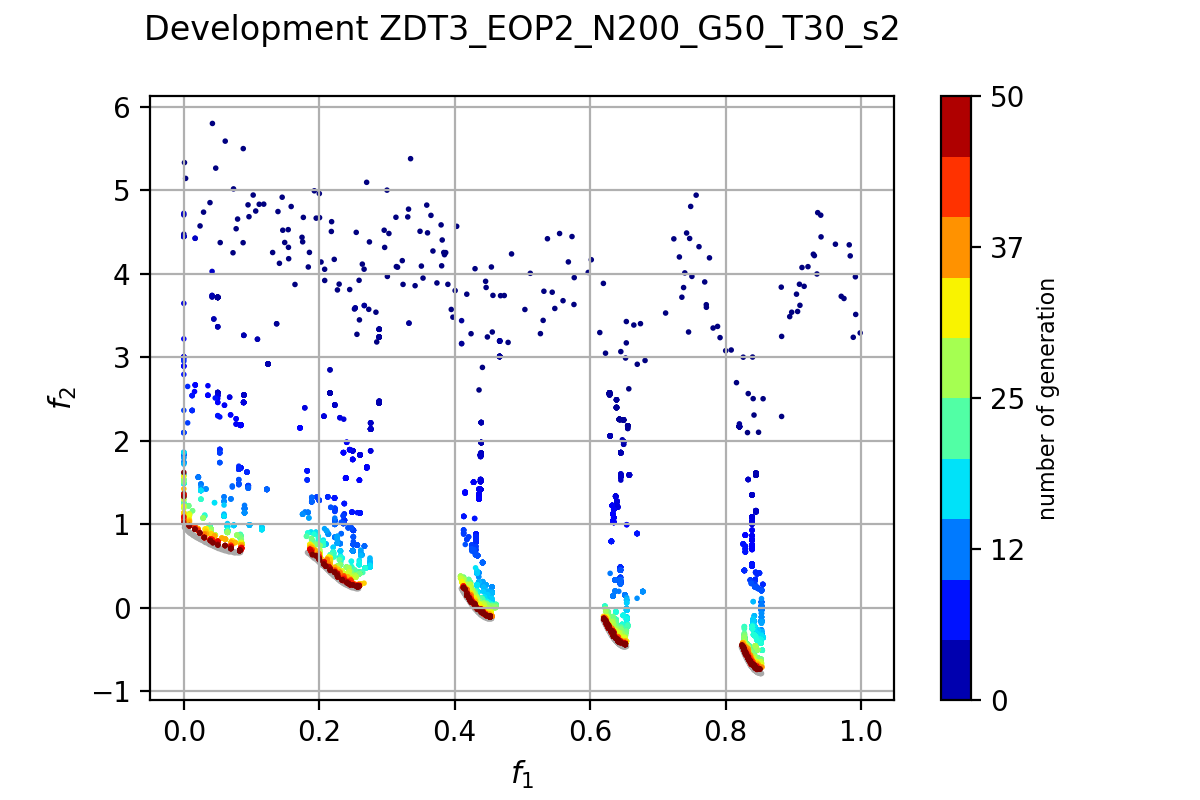
\includegraphics[scale=0.4]{figures/ZDT3_EOP2_N200_G50_T30/s2_dev.png}\\
        \includegraphics[scale=0.36]{figures/ZDT3_EOP2_N200_G50_T30/s2_nds.png}\\
        \includegraphics[scale=0.36]{figures/ZDT3_EOP2_N200_G50_T30/s2_comp.png}\\
        \caption{\centering MOEA/D + EOP2 (N200G50)}
        \label{fig:12}
    \end{figure}
    \end{minipage}\\
\end{minipage}\\



Veámos ahora unas gráficas análogas a las presentadas pero para el caso $(G=250, N=40)$ en la \hyperref[fig:11]{\textit{figura 11}} podemos notar que el comportamiento es similar al caso anterior, esto es, como se espera a través de las generaciones las soluciones van aproximándose la convergencia al igual que en el caso anterior sigue siendo es buena, sin embargo se nota que la reducción en el número de subproblemas afecta de manera notable a la dispersión, sobre todo en las últimas generaciones. Sin embargo, si miramos el frente de soluciones no dominadas, vemos que tanto en convergencia (a priori, sin otro algoritmo de referencia) que tanto el grado de convergencia de las soluciones como el grado de dispersión hacen que se aproximen en buena medida al frente real de Pareto, por lo que nos incita a pensar que la pérdida de diversidad debe darse relativamente al final porque existen soluciones buenas a lo largo prácticamente de todo el frente. Si comparamos ahora la última generación con la del algoritmo \textit{NSGA-II} (ejecutado en las mismas condiciones) podemos ver que ahora la superioridad no es tan patente como en el casi anterior y ambos algoritmos alcanzan un grado análogo de convergencia y dispersión (en este último aspecto quizá \textit{NSGA-II} parezca un poco mejor).\\


Y en último lugar comprobemos cuál es el resultado de elevar el número de subproblemas frente al número de generaciones. Dado que según hemos visto hasta ahora lo convergencia suele ser rápida, y que el número de subproblemas favorecerá la diversidad, a priori el comportamiento debería ser satisfactorio. Veámos qué ocurre para el caso $(G=250, N=40)$ en las gráficas presentadas en la \hyperref[fig:12]{\textit{figura 12}}. Podemos notar que la convergencia es bastante buena y la diversidad también permite que en las últimas generaciones se cubran los tramos del frente de manera más o menos uniforme. De hecho, si observamos el diagrama de las soluciones no dominadas podemos notar que, primero el ajuste es ligeramente peor que en los otros casos (normal dado que tiene menos generaciones para tratar de ajustarse) y la cobertura es buena y se reparte de forma más o menos uniforme. Si comparamos con la ejecución del \textit{NSGA-II} en este caso nuestro algoritmo es claramente mejor en convergencia y posiblemente en cobertura. \\

Finalmente vamos a realizar una comparativa entre los tres casos tanto para los frentes de la última generación como para los frentes \textit{NSD}. En la \hyperref[fig:13]{\textit{figura 13}} se muestran las dos gráficas de comparativa de los frente anteriormente indicados. En cuanto a las soluciones de la generación final todas se encuentran bastante superpuestas, quizá la la verde con una menor dispersión pareciendo que un número de subproblemas más elevado proporciona una mejor solución, aunque los resultados no son concluyentes y trataremos de realizar un estudio más profundo con el uso de las métricas. En cuanto al NSD,los resultados no son nada concluyentes, así que intentaremos clarificarlos con el uso de métricas y el correspondiente estudio estadístico de las mismas.\\ 

\begin{center}
\includegraphics[scale=0.8]{figures/COMPARISIONS_EOP2/GCOMP_FGEN_s2.png}\\
\end{center}
\begin{figure}[H]
\centering
\includegraphics[scale=0.8]{figures/COMPARISIONS_EOP2/GCOMP_NDS_s2.png}\\
\caption{MOEA/D + EOP2. Comparación de casos}
\label{fig:13}
\end{figure}



\subsubsection{Análisis de métricas para 10000 ev.}

Presentado el estudio preliminar anterior vamos a tratar de profundizar para exclarecer y llevar a cabo una discusión más profunda de los casos anteriores. Para ello realizaremos un estudio de algunas métricas para los casos ya presentados. Tales métricas corresponden al hipervolumen, espaciado y cover set.\\

Comencemos viendo algunas gráficas asociadas a las métricas para los casos planteados en el apartado anterior. En la \hyperref[fig:14]{figura 14} se muestra la evolución de hipervolumen y el espaciado en durante las distintas generaciones para 10 ejecuciones del algoritmo. Podemos observar que en todos los casos  el desarrollo del hipervolumen se comporta de manera bastante uniforme para todas las ejecuciones, sin embargo en el primer caso el espaciado sí varía considerablemente desde menos de 0.04 para algunas ejecuciones hasta casi 0.10 en otras.\\

Aunque no es posible hacer un análisis conjunto del hipervolumen (ya que el punto de referencia para su cálculo es distinto en cada caso) sí podemos destacar la rápida convergencia del algoritmo, menos clara que para EOP1 (hecho que destacamos también en el estudio preliminar) y el aparente estancamiento final, por lo que es preferible primar el número de subproblemas frente al número de generaciones (en valores razonables)como sugiere también el comportamiento del espaciado, que para el segundo y el tercer caso se comporta de manera más iniforme, para ambos con valores entre 0.01 y 0.03\\


\begin{figure}[H]
\centering
\includegraphics[scale=0.5]{figures/METRICS_EOP2/Hypervol_N40_G250.png}\quad 
\includegraphics[scale=0.5]{figures/METRICS_EOP2/Spacing_N40_G250.png}\\
\includegraphics[scale=0.5]{figures/METRICS_EOP2/Hypervol_N100_G100.png} \quad 
\includegraphics[scale=0.5]{figures/METRICS_EOP2/Spacing_N100_G100.png}\\
\includegraphics[scale=0.5]{figures/METRICS_EOP2/Hypervol_N200_G50.png}\quad 
\includegraphics[scale=0.5]{figures/METRICS_EOP2/Spacing_N200_G50.png}\\
\caption{MOEA/D + EOP2. Méticas para 10000 EV}
\label{fig:14}
\end{figure}


\begin{figure}[H]
\centering
\includegraphics[scale=0.35]{../METRICS_PLOTS/Hypervol_COMP_EOP2N40G250_NSGAIIN40G250.png}
\includegraphics[scale=0.35]{../METRICS_PLOTS/Spacing_COMP_EOP2N40G250_NSGAIIN40G250.png}
\includegraphics[scale=0.35]{../METRICS_PLOTS/CoverSet_COMP_EOP2N40G250_NSGAIIN40G250.png}\\
\includegraphics[scale=0.35]{../METRICS_PLOTS/Hypervol_COMP_EOP2N100G100_NSGAIIN100G100.png}
\includegraphics[scale=0.35]{../METRICS_PLOTS/Spacing_COMP_EOP2N100G100_NSGAIIN100G100.png}
\includegraphics[scale=0.35]{../METRICS_PLOTS/CoverSet_COMP_EOP2N100G100_NSGAIIN100G100.png}\\
\includegraphics[scale=0.35]{../METRICS_PLOTS/Hypervol_COMP_EOP2N200G50_NSGAIIN200G50.png}
\includegraphics[scale=0.35]{../METRICS_PLOTS/Spacing_COMP_EOP2N200G50_NSGAIIN200G50.png}
\includegraphics[scale=0.35]{../METRICS_PLOTS/CoverSet_COMP_EOP2N200G50_NSGAIIN200G50.png}\\
\caption{MOEA/D + EOP2. Comparación de métricas con NSGAII para 10000 EV.}
\label{fig:15}
\end{figure}

A continuación presentaremos algunas gráficas comparativas del comportamiento del algoritmo frente a \textit{NSGAII}. En la \hyperref[fig:15]{figura 15} se muestran las graficas con dichas comparativas en las que podemos notar que en todos los casos el espaciado en el algoritmo \textit{NSGAII} se comporta mejor que en algoritmo propuesto mientras que el hipervolumen para el caso ($N=40$, $G=250$) es favorable al algoritmo \textit{NSGAII} y favorable a nuestro algoritmo para el resto de los casos. Como vimos en el estudio preliminar el algoritmo, con los suficientes subproblemas, sí suele converger a soluciones mejores que el algoritmo \textit{NSGAII} pero también suele tender a concentrar más las soluciones.\\

Sin embargo si comprobamos la métrica cover set, sí podemos ver que en el primer caso ninguno de los frentes es dominado más de un 50\% por el otro en la mayoría de las ejecuciones, pero aún así \textit{NSGAII} tiende a quedar por debajo. Para el segundo y el tercer caso ($N100$ y $N200$) el algoritmo propuesto tiende a dominar al \textit{NSGAII}. Más concretamente para el segundo caso en casi todas las ejecuciones el frente del algoritmo \textit{NSGAII} quedó dominado por el de \textit{MOEA/D + EOP2} entre el 50\% y el 80\% de sus puntos, mientras que el frente de  \textit{NSGAII} domina al \textit{MOEA/D + EOP2} en menos de un 20\% en prácticamente todas de las ejecuciones. En el último caso, los resultados sí son claros, el frente de \textit{NSGAII} queda dominado por el de nuestro algoritmo en más de un 90\% en todas las ejecuciones mientras que el caso contrario no es apreciable para ningún punto de ninguna de las ejecuciones (en más de 1\% o 2\%). De forma que queda patente los resultados que ya comentamos para el operador EOP1 pero que en este caso se manifiestan con mayor relevancia, la cantidad de subproblemas es mucho más beneficiosa que la cantidad de generaciones.\\

Aunque en este apartado no hemos realizado (explícitamente) un análisis de las soluciones (población final y NSD) en el último apartado de esta sección presentaremos una comparativa conjunta de las últimas generaciones y de los conjuntos no dominados (NSD) para todos los casos y todos los algoritmos.	\\

\noindent\textbf{EXPERIMENTACIÓN PARA 4000 EVALUACIONES}\\

Ya presentamos para 10000 evaluaciones el comportamiento del algoritmo es adecuado, esto es, a través de las generaciones los individuos se aproximan al frente. No vamos a volver a presentarlo para el caso de 4000 evaluaciones, pues sigue lógicamente el mismo esquema (en los apéndices se presentan las gráficas que atestiguan lo expuesto). Por tanto pasaremos directamente a evaluar las métricas y a razonar directamente sobre los resultados obtenidos en dicho análisis.  \\

En la \hyperref[fig:16]{figura 16} se presentan las gráficas del desarrollo del hypervolumen y el espaciado para cada uno de los casos coniderados en las 4000 evaluaciones en contreto $(N=40, G=100)$, $(N=80, G=50)$, $(N=100, G=40)$. Como podemos apreciar el comportamiento es similar a los presentados para las 10000 evaluaciones, pero sin embargo es notable el espacio de mejora del algoritmo dado el estado de crecimiento de la curva en todos los casos, lo que parece indicar que más iteraciones y más subproblemas sí serían útiles para la mejora del algoritmo, al contrario que en EOP1 no parece haberse alcanzado el estancamiento. También es notable la gran variabilidad del espaciado dada la falta de subproblemas y generaciones, disminuyendo dicha variabilidad sensiblemente con el aumento de los subproblemas, sobre todo en el tercer caso.\\

Si realizamos una comparativa (al igual que en el caso de 10000 ev) con el algoritmo \textit{NSGAII} obtenemos conclusiones sensiblemente distintas a las presentadas para 10000 evaluaciones y para EOP1, no para el espaciado en el que \textit{NSGAII} supera (valor más bajo) a nuestro algoritmo, aunque sí se denota una notable mejora con el aumento de los subproblemas. Pero en el caso del hipervolumen en el primer caso $(N=40, G=100)$ \textit{NSGAII} supera a nuesto algoritmo en prácticamente la totalidad de las ejecuciones, mientras que en el segundo y tercer caso nuestro algoritmo consigue superarlo en este aspecto. En cuanto al cover set, para el caso $N=40$ más del 50\%   del frente (final) de nuestro algoritmo es dominado por el de \textit{NSGAII} en prácticamente todas las ejecuciones, mientras que apenas un 8\% del frente de nuestro algoritmo domina al competidor. En los otros dos casos el cover set es mucho más claro de forma que para ambos casos en buena parte de las ejecuciones más del 75\% del frente es dominado por el frente final de nuestro algoritmo, mientras que para pocas ejecuciones se produce una dominancia de \textit{NSGAII} en más de un 1\% o 2\%.\\

De todo ello destacamos la bondad de nuestro algoritmo en cuanto a la convergencia, no tanto para el espaciado (sobre todo si consideramos la última generación, si consideramos el frente NSD veremos que el espaciado mejora notablemente, presentado en la comparativa final de la \hyperref[table:1]{tabla 1}) y en cuanto al cover set, con el número adecuado de subproblemas (mejor que de generaciones) nuestro algoritmo domina practicamente en su totalidad a \textit{NSGAII}. Sí hemos de destacar que EOP se comportaba mejor ante la falta de generaciones (esto es su convergencia era más rápida). \\

\begin{figure}[H]
\centering
\includegraphics[scale=0.43]{figures/METRICS_EOP2/Hypervol_N40_G100.png} \quad 
\includegraphics[scale=0.43]{figures/METRICS_EOP2/Spacing_N40_G100.png}\\
\includegraphics[scale=0.43]{figures/METRICS_EOP2/Hypervol_N80_G50.png}\quad 
\includegraphics[scale=0.43]{figures/METRICS_EOP2/Spacing_N80_G50.png}\\
\includegraphics[scale=0.43]{figures/METRICS_EOP2/Hypervol_N100_G40.png}\quad 
\includegraphics[scale=0.43]{figures/METRICS_EOP2/Spacing_N100_G40.png}\\
\caption{MOEA/D + EOP2. Métricas para 4000EV}
\label{fig:16}
\end{figure}


\begin{figure}[H]
\centering
\includegraphics[scale=0.35]{../METRICS_PLOTS/Hypervol_COMP_EOP2N40G100_NSGAIIN40G100.png}
\includegraphics[scale=0.35]{../METRICS_PLOTS/Spacing_COMP_EOP2N40G100_NSGAIIN40G100.png}
\includegraphics[scale=0.35]{../METRICS_PLOTS/CoverSet_COMP_EOP2N40G100_NSGAIIN40G100.png}\\
\includegraphics[scale=0.35]{../METRICS_PLOTS/Hypervol_COMP_EOP2N80G50_NSGAIIN80G50.png}
\includegraphics[scale=0.35]{../METRICS_PLOTS/Spacing_COMP_EOP2N80G50_NSGAIIN80G50.png}
\includegraphics[scale=0.35]{../METRICS_PLOTS/CoverSet_COMP_EOP2N80G50_NSGAIIN80G50.png}\\
\includegraphics[scale=0.35]{../METRICS_PLOTS/Hypervol_COMP_EOP2N100G40_NSGAIIN100G40.png}
\includegraphics[scale=0.35]{../METRICS_PLOTS/Spacing_COMP_EOP2N100G40_NSGAIIN100G40.png}
\includegraphics[scale=0.35]{../METRICS_PLOTS/CoverSet_COMP_EOP2N100G40_NSGAIIN100G40.png}\\
\caption{MOEA/D + EOP2. Comparación de métricas con NSGAII para 4000 EV.}
\label{fig:17}
\end{figure}


\subsection{Evaluación MOEA/D + EOP3 con ZDT3}

De igual manera a lo presentado para EOP1 y EOP2 vamos a realizar algunas pruebas para comprobar la efectividad del algoritmo con EOP3. Tanto utilizando una capacidad de cómputo de $10000$ evaluaciones como una de $4000$ evaluaciones (con los mismos repartos ya presentados).\\

\justify
\subsubsection{Experimentación con 1OOOO ev.}

En la \hyperref[fig:18]{\textit{figura 18}} presentamos tres gráficos pertenecientes a una ejecución característica del algoritmo con el operador evolutivo EOP3, $N=100, G=100$ y $T=15$ (para todos los casos se ha tomado un $15\%$  (recuérdese que en los anexos se muestran varias ejecuciones que validan las discusiones) el primer diagrama muestra el desarrollo de las soluciones en el espacio de objetivos a lo largo de la ejecución del algoritmo (en las distintas generaciones). En él podemos apreciar que, tal como esperábamos a medida que el algoritmo avanza (pasan las generaciones) las soluciones tinden a ir convergiendo hacia el frente real de Pareto (señalado en gris), de forma muy rápida. Otro aspecto a destacar es la diversidad, en los algoritmos evolutivos es corriente que las soluciones tiendan a concentrarse (se pierde diversidad); en este caso podemos ver dicha tendencia claramente, lo que produce lógicamente, que las soluciones no se distribuyan uniformemente, dándose un fénomeno habitual en algoritmos genéticos (del que hemos heredado este tercer operador) conocido como convergencia temprana (efecto indeseable).\\

En el segundo diagrama se presenta el conjunto de las soluciones no dominadas calculadas por el algoritmo, que parece estar bastante próximo al frente real de Paretoen cuanto a convergencia, pero sí es notable la pérdida clara de uniformidad en las soluciones frente a los resultados presentados en los operadores anteriores.\\

Finalmente, presentamos una gráfica comparativa para nuestro algoritmo y para el algoritmo \textit{NSGA-II}. Para ello hemos representado las soluciones en el espacio de objetivos, las cuales corresponden a la última generación de ejecuciones en iguales condiciones $(G=100, N=100)$ para ambos algoritmos. Podemos ver que en cuanto a convergencia (proximidad al frente real) el frente del nuestro algoritmo es ligeramente mejor que el frente proporcionado por  \textit{NSGA-II} (una mayoría de los puntos rojos están por debajo de los azules), mientras que en dispersión claramente los puntos del frente de \textit{NSGA-II} se distribuyen más uniformemente que los de nuestro algoritmo.\\

Veámos ahora unas gráficas análogas a las presentadas pero para el caso $(G=250, N=40)$ en la \hyperref[fig:19]{\textit{figura 19}} podemos notar que el comportamiento es similar al caso anterior dándose exactamente el mismo efecto, pero en este caso la diferencia con\textit{NSGAII} en convergencia es menor, debido a que NSGAII ha mejorado en ese aspecto (beneficiándose mucho más de las iteraciones que nuestro algoritmo, al que no le aportan mucho, a partir de un valor razonable). Si miramos el frente de soluciones no dominadas, vemos una situación muy similar a la anterior donde la mayoría de los puntos estan situados sobre el frente pero las soluciones no están uniformemente repartidas sino que tienden a estar bastante concentradas. En comparación con \textit{NSGAII} la convergencia de nuestro algoritmo parece ligeramente mejor mientras que en la distribución es sensiblemente peor.\\

Y en último lugar comprobemos cuál es el resultado de elevar el número de subproblemas frente al número de generaciones. Dado que según hemos visto hasta ahora lo convergencia suele ser rápida, y que el número de subproblemas favorecerá la diversidad, a priori el comportamiento debería ser satisfactorio. Veámos qué ocurre para el caso $(G=250, N=40)$ en las gráficas presentadas en la \hyperref[fig:20]{\textit{figura 20}}. Podemos notar que la convergencia es bastante buena pero la concentración de las soluciones y la rápida pérdida de la diversidad es patente. De hecho, si observamos el diagrama de las soluciones no dominadas podemos seguir notando que la distribución no es para nada uniforme. Si comparamos con la ejecución del \textit{NSGA-II} en este caso nuestro algoritmo es claramente mejor en convergencia y pero no en cobertura, aunque una mayoría de los puntos (lo veremos cuando analicemos las métricas) sí parecen estar dominados por los de nuestro algoritmo. \\

\begin{minipage}[H]{\linewidth}
\begin{minipage}[b]{0.3\linewidth}

\begin{figure}[H]
        \centering
        \includegraphics[scale=0.4]{figures/ZDT3_EOP3_N100_G100_T15/s3_dev.png}\\
        \includegraphics[scale=0.36]{figures/ZDT3_EOP3_N100_G100_T15/s3_nds.png}\\
        \includegraphics[scale=0.36]{figures/ZDT3_EOP3_N100_G100_T15/s3_comp.png}\\
        \caption{\centering MOEA/D + EOP3 (N100G100)}
        \label{fig:18}
    \end{figure}
\end{minipage} \quad
\begin{minipage}[b]{0.3\linewidth}
\begin{figure}[H]
        \centering
        \includegraphics[scale=0.4]{figures/ZDT3_EOP3_N40_G250_T6/s3_dev.png}\\
        \includegraphics[scale=0.36]{figures/ZDT3_EOP3_N40_G250_T6/s3_nds.png}\\
        \includegraphics[scale=0.36]{figures/ZDT3_EOP3_N40_G250_T6/s3_comp.png}\\
        \caption{\centering MOEA/D + EOP3 (N40G250)}
        \label{fig:19}
    \end{figure}
\end{minipage} \quad
\begin{minipage}[b]{0.3\linewidth}
    \begin{figure}[H]
        \centering
        \includegraphics[scale=0.4]{figures/ZDT3_EOP3_N200_G50_T30/s3_dev.png}\\
        \includegraphics[scale=0.36]{figures/ZDT3_EOP3_N200_G50_T30/s3_nds.png}\\
        \includegraphics[scale=0.36]{figures/ZDT3_EOP3_N200_G50_T30/s3_comp.png}\\
        \caption{\centering MOEA/D + EOP3 (N200G50)}
        \label{fig:20}
    \end{figure}
    \end{minipage}\\
\end{minipage}\\

Finalmente vamos a realizar una comparativa entre los tres casos tanto para los frentes de la última generación como para los frentes \textit{NSD}. En la \hyperref[fig:21]{\textit{figura 21}} se muestran las dos gráficas de comparativa de los frente anteriormente indicados. En cuanto a las soluciones de la generación final todas se encuentran bastante superpuestas, en cuanto a convergencia todos tienen un comportamiento muy parecido, y quizá la el frente rojo, correspondiente al tercer caso denote una mejor cobertura del frente. En cuanto al NSD las sensaciones son análoga sy nada concluyentes, así que intentaremos clarificarlos con el uso de métricas y el correspondiente estudio estadístico de las mismas.\\ 

\begin{center}
\includegraphics[scale=0.8]{figures/COMPARISIONS_EOP3/GCOMP_FGEN_s3.png}\\
\end{center}
\begin{figure}[H]
\centering
\includegraphics[scale=0.8]{figures/COMPARISIONS_EOP3/GCOMP_NDS_s3.png}\\
\caption{MOEA/D + EOP3. Comparación de casos}
\label{fig:21}
\end{figure}



\subsubsection{Análisis de métricas para 10000 ev.}

Presentado el estudio preliminar anterior vamos a tratar de profundizar para exclarecer y llevar a cabo una discusión más profunda de los casos anteriores. Para ello realizaremos un estudio de algunas métricas para los casos ya presentados. Tales métricas corresponden al hipervolumen, espaciado y cover set.\\

Comencemos viendo algunas gráficas asociadas a las métricas para los casos planteados en el apartado anterior. En la \hyperref[fig:22]{figura 22} se muestra la evolución de hipervolumen y el espaciado en durante las distintas generaciones para 10 ejecuciones del algoritmo. Podemos observar que en todos los casos tanto el desarrollo del hipervolumen como el de el espaciado se comporta de forma bastante uniforme para todas las ejecuciones.\\

Aunque no es posible hacer un análisis conjunto del hipervolumen (ya que el punto de referencia para su cálculo es distinto en cada caso) sí podemos destacar la rápida convergencia del algoritmo, beneficiándose también del número de subproblemas más que de el número de generaciones observando una tendencia de estancamiento a partir de en torno al 40\% de las generaciones, en los tres casos. Observando además el beneficio del incremento del número de subproblemas en el espaciado, cuyo valor suele tender a disminuir con dicho aumento, de forma que parece claro que es preferible dedicar (de forma razonable) más parte de la potencia computacional al número de subproblemas en vez de al número de generaciones. \\

\begin{center}
\includegraphics[scale=0.5]{figures/METRICS_EOP3/Hypervol_N40_G250.png}\quad 
\includegraphics[scale=0.5]{figures/METRICS_EOP3/Spacing_N40_G250.png}\\
\includegraphics[scale=0.5]{figures/METRICS_EOP3/Hypervol_N100_G100.png} \quad 
\includegraphics[scale=0.5]{figures/METRICS_EOP3/Spacing_N100_G100.png}\\
\end{center}

\begin{figure}[H]
\centering
\includegraphics[scale=0.5]{figures/METRICS_EOP3/Hypervol_N200_G50.png}\quad 
\includegraphics[scale=0.5]{figures/METRICS_EOP3/Spacing_N200_G50.png}\\
\caption{MOEA/D + EOP3. Méticas para 10000 EV}
\label{fig:22}
\end{figure}


\begin{figure}[H]
\centering
\includegraphics[scale=0.35]{../METRICS_PLOTS/Hypervol_COMP_EOP3N40G250_NSGAIIN40G250.png}
\includegraphics[scale=0.35]{../METRICS_PLOTS/Spacing_COMP_EOP3N40G250_NSGAIIN40G250.png}
\includegraphics[scale=0.35]{../METRICS_PLOTS/CoverSet_COMP_EOP3N40G250_NSGAIIN40G250.png}\\
\includegraphics[scale=0.35]{../METRICS_PLOTS/Hypervol_COMP_EOP3N100G100_NSGAIIN100G100.png}
\includegraphics[scale=0.35]{../METRICS_PLOTS/Spacing_COMP_EOP3N100G100_NSGAIIN100G100.png}
\includegraphics[scale=0.35]{../METRICS_PLOTS/CoverSet_COMP_EOP3N100G100_NSGAIIN100G100.png}\\
\includegraphics[scale=0.35]{../METRICS_PLOTS/Hypervol_COMP_EOP3N200G50_NSGAIIN200G50.png}
\includegraphics[scale=0.35]{../METRICS_PLOTS/Spacing_COMP_EOP3N200G50_NSGAIIN200G50.png}
\includegraphics[scale=0.35]{../METRICS_PLOTS/CoverSet_COMP_EOP3N200G50_NSGAIIN200G50.png}\\
\caption{MOEA/D + EOP3. Comparación de métricas con NSGAII para 10000 EV.}
\label{fig:23}
\end{figure}

A continuación presentaremos algunas gráficas comparativas del comportamiento del algoritmo frente a \textit{NSGAII}. En la \hyperref[fig:23]{figura 23} se muestran las graficas con dichas comparativas en las que podemos notar que en todos los casos el espaciado en el algoritmo \textit{NSGAII} se comporta mejor que en algoritmo propuesto mientras que el hipervolumen el comportamiento es el contrario de forma muy notable para los casos con más subproblemas. Como vimos en el estudio preliminar el algoritmo, con los suficientes subproblemas, sí suele converger a soluciones mejores que el algoritmo \textit{NSGAII} pero también suele tender a concentrar más las soluciones.\\

Sin embargo si comprobamos la métrica cover set, sí podemos ver que en el primer caso ninguno de los frentes es dominado más de un 40\% por el otro en la mayoría de las ejecuciones, pero aún así nuestro algoritmo queda en todos los casos por debajo, no superando para ninguna de las ejecuciones el 17\% de dominancia. Para el segundo y tercer caso la situación es mucho clara, de forma que en casi todas las ejecuciones el frente del algoritmo \textit{NSGAII} quedó dominado por el de \textit{MOEA/D + EOP2} entre el 50\% y el 80\% de sus puntos, mientras que el frente de  \textit{NSGAII} domina al \textit{MOEA/D + EOP2} en menos de un 10\% en todas de las ejecuciones y para el tercer caso, el frente de \textit{NSGAII} queda dominado por el de nuestro algoritmo en más de un 95\% en todas las ejecuciones mientras que el caso contrario no es apreciable para ningún punto de ninguna de las ejecuciones (en más de 1\% o 2\%). De forma que queda patente los resultados que ya comentamos para el operador EOP1 pero que en este caso se manifiestan con mayor relevancia, la cantidad de subproblemas es mucho más beneficiosa que la cantidad de generaciones.\\

Aunque en este apartado no hemos realizado (explícitamente) un análisis de las soluciones (población final y NSD) en el último apartado de esta sección presentaremos una comparativa conjunta de las últimas generaciones y de los conjuntos no dominados (NSD) para todos los casos y todos los algoritmos.	\\

\noindent\textbf{EXPERIMENTACIÓN PARA 4000 EVALUACIONES}\\

Ya presentamos para 10000 evaluaciones el comportamiento del algoritmo es adecuado, esto es, a través de las generaciones los individuos se aproximan al frente. No vamos a volver a presentarlo para el caso de 4000 evaluaciones, pues sigue lógicamente el mismo esquema (en los apéndices se presentan las gráficas que atestiguan lo expuesto). Por tanto pasaremos directamente a evaluar las métricas y a razonar directamente sobre los resultados obtenidos en dicho análisis.  \\

En la \hyperref[fig:24]{figura 24} se presentan las gráficas del desarrollo del hypervolumen y el espaciado para cada uno de los casos coniderados en las 4000 evaluaciones en contreto $(N=40, G=100)$, $(N=80, G=50)$, $(N=100, G=40)$. Como podemos apreciar el comportamiento es similar a los presentados para las 10000 evaluaciones, de hecho se empieza a atisvar la mencionada llegada a la zona de estanco y sí es notable la gran variabilidad del espaciado dada la falta de subproblemas y generaciones, disminuyendo dicha variabilidad ligeramente con el aumento de los subproblemas..\\

Si realizamos una comparativa (al igual que en el caso de 10000 ev) con el algoritmo \textit{NSGAII} obtenemos conclusiones análogas a las presentadas para 10000 evaluaciones, de forma que en el espaciado \textit{NSGAII} supera (valor más bajo) a nuestro algoritmo, aunque sí se denota una mejora con el aumento de los subproblemas. En el caso del hipervolumen nuestro algoritmo supera a \textit{NSGAII} en prácticamente la totalidad de las ejecuciones. En cuanto al cover set,  para el caso $N=40$ más del 50\%  del frente (final) de \textit{NSGAII} es dominado por nuestro algoritmo en todas las ejecuciones, mientras que apenas un no se aprecia (ni un 1\% o 2\%) del caso contrario. En los otros casos la situación es más clara dominando nuestro algoritmo más del 90\% del frente de \textit{NSGAII} en todas las ejecuciones y siendo inapreciable el caso opuesto\\

De todo ello destacamos la bondad de nuestro algoritmo en cuanto a la convergencia, no  para el espaciado  y en cuanto al cover set, con el número adecuado de subproblemas (mejor que de generaciones) nuestro algoritmo domina practicamente en su totalidad a \textit{NSGAII}. Si destacamos frente a EOP1 y EOP2 la severa pérdida de diversidad que lo lleva a un reparto poco uniforme de las soluciones a lo largo del frente.\\

\begin{figure}[H]
\centering
\includegraphics[scale=0.43]{figures/METRICS_EOP3/Hypervol_N40_G100.png} \quad 
\includegraphics[scale=0.43]{figures/METRICS_EOP3/Spacing_N40_G100.png}\\
\includegraphics[scale=0.43]{figures/METRICS_EOP3/Hypervol_N80_G50.png}\quad 
\includegraphics[scale=0.43]{figures/METRICS_EOP3/Spacing_N80_G50.png}\\
\includegraphics[scale=0.43]{figures/METRICS_EOP3/Hypervol_N100_G40.png}\quad 
\includegraphics[scale=0.43]{figures/METRICS_EOP3/Spacing_N100_G40.png}\\
\caption{MOEA/D + EOP3. Métricas para 4000EV}
\label{fig:24}
\end{figure}


\begin{figure}[H]
\centering
\includegraphics[scale=0.35]{../METRICS_PLOTS/Hypervol_COMP_EOP3N40G100_NSGAIIN40G100.png}
\includegraphics[scale=0.35]{../METRICS_PLOTS/Spacing_COMP_EOP3N40G100_NSGAIIN40G100.png}
\includegraphics[scale=0.35]{../METRICS_PLOTS/CoverSet_COMP_EOP3N40G100_NSGAIIN40G100.png}\\
\includegraphics[scale=0.35]{../METRICS_PLOTS/Hypervol_COMP_EOP3N80G50_NSGAIIN80G50.png}
\includegraphics[scale=0.35]{../METRICS_PLOTS/Spacing_COMP_EOP3N80G50_NSGAIIN80G50.png}
\includegraphics[scale=0.35]{../METRICS_PLOTS/CoverSet_COMP_EOP3N80G50_NSGAIIN80G50.png}\\
\includegraphics[scale=0.35]{../METRICS_PLOTS/Hypervol_COMP_EOP3N100G40_NSGAIIN100G40.png}
\includegraphics[scale=0.35]{../METRICS_PLOTS/Spacing_COMP_EOP3N100G40_NSGAIIN100G40.png}
\includegraphics[scale=0.35]{../METRICS_PLOTS/CoverSet_COMP_EOP3N100G40_NSGAIIN100G40.png}\\
\caption{MOEA/D + EOP3. Comparación de métricas con NSGAII para 4000 EV.}
\label{fig:25}
\end{figure}

\subsection{Comparativa final de los algoritmos}

Para terminar el análisis vamos a presentar un análisis estadístico de las métricas de hipervolumen, espaciado y coverset sobre las soluciones proporcionadas por los distintos algoritmos, que acrediten (o desmientan) los resultados que venimos presentando hasta el momento. Comencemos presentando los resultados para las generaciones finales (incluyendo a \textit{NSGAII}) y después presentaremos también los resultados dados por NDS. Para cada una de las tablas se ha tomado el mismo punto de referencia para la evaluación del hipervolumen, de forma que los resultados aquí presentados son totalmente comparables entre sí).\\

En la \hyperref[table:1]{tabla 1} se presentan los resultados de la comparativa de las métricas de hipervolumen y espaciado para 4000 EV. Podemos ver en la misma que el algoritmo \textit{MOEA/D EOP1} (con $N=100, G=40$), aunque en el espaciado como venimos presentando el mejor es \textit{NSGAII}. Sin embargo, es mucho más considerable la ganancia hipervolumen de nuestro algoritmo frente a la pérdida de espaciado. Tanto es así que si acudimos a la \hyperref[table:5]{tabla 5} vemos que en cuanto al cover set, vemos que el frente de nuestro algoritmo domina al 100\% del frente de \textit{NSGAII} en el 100\% de las ejecuciones. Por lo tanto podemos considerar que bajo 4000 evaluaciones nuestro algoritmo es mejor que \textit{NSGAII} y además que, como ya hemos resaltado, es mucho más conveniente primar el número de subproblemas frente al número de generaciones. Además los resultados de las tablas refuerzan todos los análisis que hemos venido presentando tanto para \textit{EOP1}, \textit{EOP2} y \textit{EOP3}. \\

Si pasamos ahora a evaluar estas mismas métricas sobre 10000 evaluaciones, en la \hyperref[table:2]{tabla 2} se presentan los resultados de la comparativa de las métricas de hipervolumen y espaciado y en la \hyperref[table:6]{tabla 6} el cover set, podemos ver reflejada una situación análoga a la presentada para 4000EV. En el que \textit{EOP1} vuelve a ser el mejor en cuanto a hipervolumen y \textit{NSGAII} en cuanto a espaciado, repitiéndose también la dominancia de nuestro algoritmo sobre el competidor en más del 99\% del frente casi la totalidad de las ejecuciones y dándose el caso contrario para el 0\% del frente en la totalidad de las ejecuciones, por lo que nuestro algoritmo vence también a \textit{NSGAII} con un mayor poder computacional y siempre mejorando con el mayor uso  un mayor número de subproblemas (aunque en este caso los casos $N100$ y $N200$ son prácticamente equivalentes.\\


Finalmente vamos a comentar algunos resultados acerca de las soluciones dada por los frentes NDS. En la \hyperref[table:2]{tabla 2} se presentan los resultados de la comparativa de las métricas de hipervolumen y espaciado y en la \hyperref[table:6]{tabla 6} el cover set para los casos con 4000EV. Podemos observar que en este aspecto EOP1 vuelve a ser el mejor valorado frente a EOP2 y EOP3 tanto en hipervolumen como en espaciado. En hipervolumen si es notable que el operador EOP3 es prcticamente equivalente a EOP1 pero en cuanto al espaciado EOP1 es claramente vencedor, logrando los mejores valores para el caso con 100 subproblemas, logrando valores comparables en espaciado a los presentados para la generación final de \textit{NSGAII}. En cuanto al cover set,  vemos que es clara la dominancia de EOP1 y EOP3 sobre EOP2, pero entre ellos es menos clara (a pesar de que EOP3 tiende a dominar a EOP1 en más del 40\% del frente). En el caso de 10000EV, los resultados son similares a los presentados para 40000EV, aunque disminuyendo la dominancia en coverset de EOP3 a EOP1.\\ 

\section{Conclusion final}

Después de los resultados presentados de la experimentación realizada, es destacable la mejora de nuestro algoritmo frente a \textit{NSGAII} especialmente en el caso de \textit{EOP1}. Destacando, además, la rápida convergencia de nuestro algoritmo comprobando complementariamente el beneficio del aumento del número de subproblemas tanto para la convergencia, como por supuesto para el espaciado, de forma que a un poder computacional de 4000EV el algoritmo con mejor comportamiento corresponde a \textit{MOEA/D + EOP1} con una población de 100 individuos y 40 generaciones mientras que para 10000EV el mejor resultado se alcanzó con ese mismo algoritmo y con 200 individuos y 50 generaciones. Además los otros dos operadores evaluados demostraron un comportamiento aceptable, sobre todo en las 10000 evaluaciones, concretamente EOP3 quien (aunque con falta de diversidad) consiguió resultados muy buenos.Por último destacar el beneficio del NDS, en cuanto a la cobertura del frente, sin descompensar la convergencia, que proporcionó, sobre todo para EOP1 una aproximación muy cercana al frente real de Pareto.\\


\begin{table}[H]
\centering
\renewcommand{\arraystretch}{1.5}
\begin{tabular}{ccccccc}
\toprule
ALGORITHM  &    N &    G &   Hv\_mean &    Hv\_std &  Spc\_mean &   Spc\_std \\
\midrule
MOEA/D EOP1 &   40 &  100 &  2.088514 &  0.015041 &  0.038675 &  0.001963 \\
MOEA/D EOP1 &   80 &   50 &  2.107404 &  0.009019 &  0.020931 &  0.002098 \\
MOEA/D EOP1 &  100 &   40 &  \textbf{2.103889} &  \textbf{0.004384} &  0.016192 &  0.002490 \\
MOEA/D EOP2 &   40 &  100 &  1.899492 &  0.059507 &  0.063062 &  0.019576 \\
MOEA/D EOP2 &   80 &   50 &  1.929259 &  0.064898 &  0.045417 &  0.014444 \\
MOEA/D EOP2 &  100 &   40 &  1.938250 &  0.070247 &  0.042124 &  0.010837 \\
MOEA/D EOP3 &   40 &  100 &  2.106688 &  0.034493 &  0.055301 &  0.027549 \\
MOEA/D EOP3 &   80 &   50 &  2.121596 &  0.023985 &  0.032382 &  0.009011 \\
MOEA/D EOP3 &  100 &   40 &  2.119973 &  0.010458 &  0.032826 &  0.013621 \\
NSGAII &   40 &  100 &  2.012664 &  0.023211 &  0.012071 &  0.002019 \\
NSGAII &   80 &   50 &  1.790951 &  0.047534 &  0.009881 &  0.002221 \\
NSGAII &  100 &   40 &  1.745769 &  0.036844 &  \textbf{0.008174} &  \textbf{0.001572} \\
\bottomrule
\end{tabular}
\caption{ZDT3- Comparativa completa Hipervol. y Spacing (FGEN, 4000EV)}
\label{table:1}
\end{table}

\begin{table}[H]
\centering
\renewcommand{\arraystretch}{1.5}
\begin{tabular}{ccccccc}
\toprule
ALGORITHM &    N &    G &   Hv\_mean &    Hv\_std &  Spc\_mean &   Spc\_std \\
\midrule
MOEA/D EOP1 &   40 &  250 &  1.684281 &  0.001819 &  0.037795 &  0.001208 \\
MOEA/D EOP1 &  100 &  100 &  1.693973 &  0.001051 &  0.015474 &  0.000347 \\
MOEA/D EOP1 &  200 &   50 &  \textbf{1.694149} &  \textbf{0.00286}7 &  0.008268 &  0.000891 \\
MOEA/D EOP2 &   40 &  250 &  1.660451 &  0.008558 &  0.052216 &  0.015527 \\
MOEA/D EOP2 &  100 &  100 &  1.660273 &  0.047921 &  0.022429 &  0.008742 \\
MOEA/D EOP2 &  200 &   50 &  1.675938 &  0.006607 &  0.015855 &  0.008601 \\
MOEA/D EOP3 &   40 &  250 &  1.682167 &  0.002680 &  0.043343 &  0.007077 \\
MOEA/D EOP3 &  100 &  100 &  1.688566 &  0.002852 &  0.022407 &  0.006816 \\
MOEA/D EOP3 &  200 &   50 &  1.686791 &  0.005307 &  0.016195 &  0.005595 \\
NSGAII &   40 &  250 &  1.685467 &  0.003161 &  0.013168 &  0.001379 \\
NSGAII &  100 &  100 &  1.656455 &  0.006912 &  0.004888 &  0.000580 \\
NSGAII &  200 &   50 &  1.522302 &  0.017832 &  \textbf{0.004105} &  \textbf{0.000507} \\
\bottomrule
\end{tabular}

\caption{ZDT3- Comparativa completa Hipervol. y Spacing (FGEN, 10000EV)}
\label{table:2}
\end{table}

\begin{table}[H]
\centering
\renewcommand{\arraystretch}{1.5}
\begin{tabular}{ccccccc}
\toprule
   ALGORITHM &    N &    G &   Hv\_mean &    Hv\_std &  Spc\_mean &   Spc\_std \\
\midrule
 MOEA/D EOP1 &   40 &  100 &  1.451592 &  0.030917 &  0.027312 &  0.017374 \\
 MOEA/D EOP1 &   80 &   50 &  \textbf{1.497310} &  \textbf{0.007318} &  0.009470 &  0.002279 \\
 MOEA/D EOP1 &  100 &   40 &  1.496890 &  0.004449 &  \textbf{0.008987} &  \textbf{0.001489} \\
 MOEA/D EOP2 &   40 &  100 &  1.302208 &  0.055153 &  0.024994 &  0.009511 \\
 MOEA/D EOP2 &   80 &   50 &  1.334811 &  0.064589 &  0.022065 &  0.007143 \\
 MOEA/D EOP2 &  100 &   40 &  1.344495 &  0.072631 &  0.021256 &  0.011216 \\
 MOEA/D EOP3 &   40 &  100 &  1.449614 &  0.083014 &  0.098708 &  0.068756 \\
 MOEA/D EOP3 &   80 &   50 &  1.496368 &  0.043114 &  0.079722 &  0.058070 \\
 MOEA/D EOP3 &  100 &   40 &  1.498124 &  0.029528 &  0.062702 &  0.025272 \\
\bottomrule
\end{tabular}

\caption{ZDT3- Comparativa completa Hipervol. y Spacing (NDS, 4000EV)}
\label{table:3}
\end{table}

\begin{table}[H]
\centering
\renewcommand{\arraystretch}{1.5}
\begin{tabular}{ccccccc}
\toprule
   ALGORITHM &    N &    G &   Hv\_mean &    Hv\_std &  Spc\_mean &   Spc\_std \\
\midrule
 MOEA/D EOP1 &   40 &  250 &  1.235404 &  0.248486 &  0.014032 &  0.016374 \\
 MOEA/D EOP1 &  100 &  100 &  1.259206 &  0.266413 &  0.004887 &  0.003128 \\
 MOEA/D EOP1 &  200 &   50 &  \textbf{1.263475} &  \textbf{0.271422} &  \textbf{0.003192} &  \textbf{0.000780} \\
 MOEA/D EOP2 &   40 &  250 &  1.223784 &  0.249435 &  0.017460 &  0.015928 \\
 MOEA/D EOP2 &  100 &  100 &  1.232368 &  0.273584 &  0.006281 &  0.001798 \\
 MOEA/D EOP2 &  200 &   50 &  1.247745 &  0.273041 &  0.005406 &  0.000924 \\
 MOEA/D EOP3 &   40 &  250 &  1.213916 &  0.233524 &  0.064273 &  0.069826 \\
 MOEA/D EOP3 &  100 &  100 &  1.236160 &  0.251089 &  0.055110 &  0.052205 \\
 MOEA/D EOP3 &  200 &   50 &  1.250131 &  0.262513 &  0.042286 &  0.036711 \\
\bottomrule
\end{tabular}
\caption{ZDT3- Comparativa completa Hipervol. y Spacing (NDS, 10000EV)}
\label{table:4}
\end{table}

\begin{table}[H]
\centering
\renewcommand{\arraystretch}{1.5}
\begin{tabular}{cccccccc}
\toprule
 \multirow{2}{*}{ALG1} &    \multirow{2}{*}{ALG2} &    \multirow{2}{*}{N} &    \multirow{2}{*}{G} &  \multicolumn{2}{c}{c(ALG2, ALG1)} &  \multicolumn{2}{c}{c(ALG1, ALG2)} \\ \cline{5-6} \cline{7-8}
   &   &   &   &  Mean &  Std &  Mean &  Std \\
\midrule
 EOP1 &    EOP2 &   40 &  100 &            0.000000 &           0.000000 &            0.974490 &       1.110223e-16 \\
 EOP1 &    EOP2 &   80 &   50 &            0.000000 &           0.000000 &            0.974490 &       1.110223e-16 \\
 EOP1 &    EOP2 &  100 &   40 &            0.000000 &           0.000000 &            0.974490 &       1.110223e-16 \\
 EOP1 &    EOP3 &   40 &  100 &            0.000000 &           0.000000 &            0.974490 &       1.110223e-16 \\
 EOP1 &    EOP3 &   80 &   50 &            0.000000 &           0.000000 &            0.974490 &       1.110223e-16 \\
 EOP1 &    EOP3 &  100 &   40 &            0.000000 &           0.000000 &            0.974490 &       1.110223e-16 \\
 EOP1 &  NSGAII &   40 &  100 &            0.008655 &           0.018388 &            0.769936 &       1.416819e-01 \\
 EOP1 &  NSGAII &   80 &   50 &            0.000000 &           0.000000 &            1.000000 &       0.000000e+00 \\
 EOP1 &  NSGAII &  100 &   40 &            0.000000 &           0.000000 &            1.000000 &       0.000000e+00 \\
 EOP2 &    EOP3 &   40 &  100 &            0.000000 &           0.000000 &            1.000000 &       0.000000e+00 \\
 EOP2 &    EOP3 &   80 &   50 &            0.000000 &           0.000000 &            1.000000 &       0.000000e+00 \\
 EOP2 &    EOP3 &  100 &   40 &            0.000000 &           0.000000 &            1.000000 &       0.000000e+00 \\
 EOP2 &  NSGAII &   40 &  100 &            0.696330 &           0.245986 &            0.050897 &       1.056916e-01 \\
 EOP2 &  NSGAII &   80 &   50 &            0.042708 &           0.100827 &            0.794910 &       1.437527e-01 \\
 EOP2 &  NSGAII &  100 &   40 &            0.040767 &           0.089379 &            0.842722 &       2.059881e-01 \\
 EOP3 &  NSGAII &   40 &  100 &            0.000000 &           0.000000 &            0.772244 &       1.208985e-01 \\
 EOP3 &  NSGAII &   80 &   50 &            0.000000 &           0.000000 &            0.989873 &       2.320291e-02 \\
 EOP3 &  NSGAII &  100 &   40 &            0.000000 &           0.000000 &            0.992815 &       1.531966e-02 \\
\bottomrule
\end{tabular}
\caption{ZDT3- Comparativa completa Cover Set (FGEN, 4000EV)}
\label{table:5}
\end{table}

\begin{table}[H]
\centering
\renewcommand{\arraystretch}{1.5}
\begin{tabular}{cccccccc}
\toprule
 \multirow{2}{*}{ALG1} &    \multirow{2}{*}{ALG2} &    \multirow{2}{*}{N} &    \multirow{2}{*}{G} &  \multicolumn{2}{c}{c(ALG2, ALG1)} &  \multicolumn{2}{c}{c(ALG1, ALG2)} \\ \cline{5-6} \cline{7-8}
   &   &   &   &  Mean &  Std &  Mean &  Std \\
\midrule
 EOP1 &    EOP2 &   40 &  250 &            0.000000 &           0.000000 &            0.989899 &       1.110223e-16 \\
 EOP1 &    EOP2 &  100 &  100 &            0.000000 &           0.000000 &            0.989899 &       1.110223e-16 \\
 EOP1 &    EOP2 &  200 &   50 &            0.000000 &           0.000000 &            0.989899 &       1.110223e-16 \\
 EOP1 &    EOP3 &   40 &  250 &            0.000000 &           0.000000 &            0.989899 &       1.110223e-16 \\
 EOP1 &    EOP3 &  100 &  100 &            0.000000 &           0.000000 &            0.989899 &       1.110223e-16 \\
 EOP1 &    EOP3 &  200 &   50 &            0.000000 &           0.000000 &            0.989899 &       1.110223e-16 \\
 EOP1 &  NSGAII &   40 &  250 &            0.053730 &           0.054245 &            0.220000 &       7.483315e-02 \\
 EOP1 &  NSGAII &  100 &  100 &            0.000000 &           0.000000 &            0.907915 &       3.822231e-02 \\
 EOP1 &  NSGAII &  200 &   50 &            0.000000 &           0.000000 &            0.992347 &       2.295918e-02 \\
 EOP2 &    EOP3 &   40 &  250 &            0.000000 &           0.000000 &            1.000000 &       0.000000e+00 \\
 EOP2 &    EOP3 &  100 &  100 &            0.000000 &           0.000000 &            1.000000 &       0.000000e+00 \\
 EOP2 &    EOP3 &  200 &   50 &            0.000000 &           0.000000 &            1.000000 &       0.000000e+00 \\
 EOP2 &  NSGAII &   40 &  250 &            0.260153 &           0.118778 &            0.040000 &       4.636809e-02 \\
 EOP2 &  NSGAII &  100 &  100 &            0.136465 &           0.281695 &            0.576990 &       2.292387e-01 \\
 EOP2 &  NSGAII &  200 &   50 &            0.000000 &           0.000000 &            0.965804 &       4.469600e-02 \\
 EOP3 &  NSGAII &   40 &  250 &            0.040089 &           0.032455 &            0.255000 &       7.053368e-02 \\
 EOP3 &  NSGAII &  100 &  100 &            0.008386 &           0.018737 &            0.610813 &       9.586192e-02 \\
 EOP3 &  NSGAII &  200 &   50 &            0.000000 &           0.000000 &            0.987302 &       1.287349e-02 \\
\bottomrule
\end{tabular}
\caption{ZDT3- Comparativa completa Cover Set (FGEN, 10000EV)}
\label{table:6}
\end{table}

\begin{table}[H]
\centering
\renewcommand{\arraystretch}{1.5}
\begin{tabular}{cccccccc}
\toprule
 \multirow{2}{*}{ALG1} &    \multirow{2}{*}{ALG2} &    \multirow{2}{*}{N} &    \multirow{2}{*}{G} &  \multicolumn{2}{c}{c(ALG2, ALG1)} &  \multicolumn{2}{c}{c(ALG1, ALG2)} \\ \cline{5-6} \cline{7-8}
   &   &   &   &  Mean &  Std &  Mean &  Std \\
\midrule
 EOP1 &  EOP2 &   40 &  100 &            0.000000 &           0.000000 &            0.995505 &           0.008991 \\
 EOP1 &  EOP2 &   80 &   50 &            0.000000 &           0.000000 &            0.997826 &           0.006522 \\
 EOP1 &  EOP2 &  100 &   40 &            0.002469 &           0.007407 &            0.993750 &           0.018750 \\
 EOP1 &  EOP3 &   40 &  100 &            0.491354 &           0.096355 &            0.048016 &           0.060577 \\
 EOP1 &  EOP3 &   80 &   50 &            0.454795 &           0.087867 &            0.027795 &           0.028894 \\
 EOP1 &  EOP3 &  100 &   40 &            0.414962 &           0.051668 &            0.049302 &           0.048648 \\
 EOP2 &  EOP3 &   40 &  100 &            0.915397 &           0.097093 &            0.003846 &           0.011538 \\
 EOP2 &  EOP3 &   80 &   50 &            0.921391 &           0.085503 &            0.000000 &           0.000000 \\
 EOP2 &  EOP3 &  100 &   40 &            0.842845 &           0.108491 &            0.005556 &           0.016667 \\
\bottomrule
\end{tabular}
\caption{ZDT3- Comparativa completa Cover Set (NDS, 4000EV)}
\label{table:7}
\end{table}

\begin{table}[H]
\centering
\renewcommand{\arraystretch}{1.5}
\begin{tabular}{cccccccc}
\toprule
 \multirow{2}{*}{ALG1} &    \multirow{2}{*}{ALG2} &    \multirow{2}{*}{N} &    \multirow{2}{*}{G} &  \multicolumn{2}{c}{c(ALG2, ALG1)} &  \multicolumn{2}{c}{c(ALG1, ALG2)} \\ \cline{5-6} \cline{7-8}
   &   &   &   &  Mean &  Std &  Mean &  Std \\
\midrule
 EOP1 &  EOP2 &   40 &  250 &            0.024549 &           0.020495 &            0.873728 &           0.080861 \\
 EOP1 &  EOP2 &  100 &  100 &            0.018487 &           0.022481 &            0.910285 &           0.068369 \\
 EOP1 &  EOP2 &  200 &   50 &            0.020209 &           0.019274 &            0.877289 &           0.088478 \\
 EOP1 &  EOP3 &   40 &  250 &            0.247131 &           0.056417 &            0.131976 &           0.067172 \\
 EOP1 &  EOP3 &  100 &  100 &            0.247053 &           0.049638 &            0.084933 &           0.036117 \\
 EOP1 &  EOP3 &  200 &   50 &            0.290046 &           0.064070 &            0.082858 &           0.032555 \\
 EOP2 &  EOP3 &   40 &  250 &            0.541899 &           0.074144 &            0.032363 &           0.023784 \\
 EOP2 &  EOP3 &  100 &  100 &            0.599404 &           0.152908 &            0.019685 &           0.016970 \\
 EOP2 &  EOP3 &  200 &   50 &            0.603076 &           0.116967 &            0.025308 &           0.022203 \\
\bottomrule
\end{tabular}
\caption{ZDT3- Comparativa completa Cover Set (NDS, 10000EV)}
\label{table:8}
\end{table}






\bibliography{references} 
\bibliographystyle{IEEEtran}

% \appendix
% \section{Graficas de evaluación de MOEA/D + EPO1 PARA ZDT3}
% 
\begin{figure}[H]
    \centering
    \begin{tabular}{c c}
    \includegraphics[scale=0.45]{figures/ZDT3_EOP1_N100_G100_T15/s1_dev.png} &
    \includegraphics[scale=0.45]{figures/ZDT3_EOP1_N100_G100_T15/s1_nds.png}\\
    \includegraphics[scale=0.45]{figures/ZDT3_EOP1_N100_G100_T15/s5_dev.png} &
    \includegraphics[scale=0.45]{figures/ZDT3_EOP1_N100_G100_T15/s5_nds.png}\\
    \includegraphics[scale=0.45]{figures/ZDT3_EOP1_N100_G100_T15/s8_dev.png} &
    \includegraphics[scale=0.45]{figures/ZDT3_EOP1_N100_G100_T15/s8_nds.png}\\
    \includegraphics[scale=0.45]{figures/ZDT3_EOP1_N100_G100_T15/s99_dev.png} &
    \includegraphics[scale=0.45]{figures/ZDT3_EOP1_N100_G100_T15/s99_nds.png}\\
    \end{tabular}
    \caption{MOEA/D + EOP1 para ZDT3 con N100 G100 T15 }
    \label{fig:2}
\end{figure}

\begin{figure}[H]
    \centering
    \begin{tabular}{c c}
    \includegraphics[scale=0.5]{figures/ZDT3_EOP1_N100_G100_T15/s1_comp.png} &
    \includegraphics[scale=0.5]{figures/ZDT3_EOP1_N100_G100_T15/s2_comp.png}\\
    \includegraphics[scale=0.5]{figures/ZDT3_EOP1_N100_G100_T15/s3_comp.png} &
    \includegraphics[scale=0.5]{figures/ZDT3_EOP1_N100_G100_T15/s4_comp.png}\\
    \includegraphics[scale=0.5]{figures/ZDT3_EOP1_N100_G100_T15/s5_comp.png} &
    \includegraphics[scale=0.5]{figures/ZDT3_EOP1_N100_G100_T15/s7_comp.png}\\
    \includegraphics[scale=0.5]{figures/ZDT3_EOP1_N100_G100_T15/s9_comp.png} &
    \includegraphics[scale=0.5]{figures/ZDT3_EOP1_N100_G100_T15/s99_comp.png}\\
    \end{tabular}
    \caption{\centering MOEA/D + EOP1 vs NSGAII para ZDT3 con N100 G100 T15}
    \label{fig:3}
\end{figure}

\begin{figure}[H]
    \centering
    \begin{tabular}{c c}
    \includegraphics[scale=0.5]{figures/ZDT3_EOP1_N40_G250_T6/s1_dev.png} &
    \includegraphics[scale=0.5]{figures/ZDT3_EOP1_N40_G250_T6/s1_nds.png}\\
    \includegraphics[scale=0.5]{figures/ZDT3_EOP1_N40_G250_T6/s5_dev.png} &
    \includegraphics[scale=0.5]{figures/ZDT3_EOP1_N40_G250_T6/s5_nds.png}\\
    \includegraphics[scale=0.5]{figures/ZDT3_EOP1_N40_G250_T6/s8_dev.png} &
    \includegraphics[scale=0.5]{figures/ZDT3_EOP1_N40_G250_T6/s8_nds.png}\\
    \includegraphics[scale=0.5]{figures/ZDT3_EOP1_N40_G250_T6/s99_dev.png} &
    \includegraphics[scale=0.5]{figures/ZDT3_EOP1_N40_G250_T6/s99_nds.png}\\
    \end{tabular}
    \caption{MOEA/D + EOP1 para ZDT3 con N40 G250 T6 }
    \label{fig:4}
\end{figure}


\begin{figure}[H]
    \centering
    \begin{tabular}{c c}
    \includegraphics[scale=0.5]{figures/ZDT3_EOP1_N40_G250_T6/s1_comp.png} &
    \includegraphics[scale=0.5]{figures/ZDT3_EOP1_N40_G250_T6/s2_comp.png}\\
    \includegraphics[scale=0.5]{figures/ZDT3_EOP1_N40_G250_T6/s3_comp.png} &
    \includegraphics[scale=0.5]{figures/ZDT3_EOP1_N40_G250_T6/s4_comp.png}\\
    \includegraphics[scale=0.5]{figures/ZDT3_EOP1_N40_G250_T6/s5_comp.png} &
    \includegraphics[scale=0.5]{figures/ZDT3_EOP1_N40_G250_T6/s7_comp.png}\\
    \includegraphics[scale=0.5]{figures/ZDT3_EOP1_N40_G250_T6/s9_comp.png} &
    \includegraphics[scale=0.5]{figures/ZDT3_EOP1_N40_G250_T6/s99_comp.png}\\
    \end{tabular}
    \caption{\centering MOEA/D + EOP1 vs NSGAII para ZDT3 con N40 G250 T6}
    \label{fig:5}
\end{figure}

\begin{figure}[H]
    \centering
    \begin{tabular}{c c}
    \includegraphics[scale=0.5]{figures/ZDT3_EOP1_N200_G50_T30/s1_dev.png} &
    \includegraphics[scale=0.5]{figures/ZDT3_EOP1_N200_G50_T30/s1_nds.png}\\
    \includegraphics[scale=0.5]{figures/ZDT3_EOP1_N200_G50_T30/s5_dev.png} &
    \includegraphics[scale=0.5]{figures/ZDT3_EOP1_N200_G50_T30/s5_nds.png}\\
    \includegraphics[scale=0.5]{figures/ZDT3_EOP1_N200_G50_T30/s8_dev.png} &
    \includegraphics[scale=0.5]{figures/ZDT3_EOP1_N200_G50_T30/s8_nds.png}\\
    \includegraphics[scale=0.5]{figures/ZDT3_EOP1_N200_G50_T30/s99_dev.png} &
    \includegraphics[scale=0.5]{figures/ZDT3_EOP1_N200_G50_T30/s99_nds.png}\\
    \end{tabular}
    \caption{MOEA/D + EOP1 para ZDT3 con N200 G50 T30 }
    \label{fig:6}
\end{figure}

\begin{figure}[H]
    \centering
    \begin{tabular}{c c}
    \includegraphics[scale=0.5]{figures/ZDT3_EOP1_N200_G50_T30/s1_comp.png} &
    \includegraphics[scale=0.5]{figures/ZDT3_EOP1_N200_G50_T30/s2_comp.png}\\
    \includegraphics[scale=0.5]{figures/ZDT3_EOP1_N200_G50_T30/s3_comp.png} &
    \includegraphics[scale=0.5]{figures/ZDT3_EOP1_N200_G50_T30/s4_comp.png}\\
    \includegraphics[scale=0.5]{figures/ZDT3_EOP1_N200_G50_T30/s5_comp.png} &
    \includegraphics[scale=0.5]{figures/ZDT3_EOP1_N200_G50_T30/s7_comp.png}\\
    \includegraphics[scale=0.5]{figures/ZDT3_EOP1_N200_G50_T30/s9_comp.png} &
    \includegraphics[scale=0.5]{figures/ZDT3_EOP1_N200_G50_T30/s99_comp.png}\\
    \end{tabular}
    \caption{\centering MOEA/D + EOP1 vs NSGAII para ZDT3 con N200 G50 T30}
    \label{fig:7}
\end{figure}

\begin{figure}[H]
    \centering
    \begin{tabular}{c c}
    \includegraphics[scale=0.5]{figures/ZDT3_EOP1_N80_G50_T12/s1_dev.png} &
    \includegraphics[scale=0.5]{figures/ZDT3_EOP1_N80_G50_T12/s1_nds.png}\\
    \includegraphics[scale=0.5]{figures/ZDT3_EOP1_N80_G50_T12/s5_dev.png} &
    \includegraphics[scale=0.5]{figures/ZDT3_EOP1_N80_G50_T12/s5_nds.png}\\
    \includegraphics[scale=0.5]{figures/ZDT3_EOP1_N80_G50_T12/s8_dev.png} &
    \includegraphics[scale=0.5]{figures/ZDT3_EOP1_N80_G50_T12/s8_nds.png}\\
    \includegraphics[scale=0.5]{figures/ZDT3_EOP1_N80_G50_T12/s99_dev.png} &
    \includegraphics[scale=0.5]{figures/ZDT3_EOP1_N80_G50_T12/s99_nds.png}\\
    \end{tabular}
    \caption{MOEA/D + EOP1 para ZDT3 con N80 G50 T12 }
    \label{fig:8}
\end{figure}

\begin{figure}[H]
    \centering
    \begin{tabular}{c c}
    \includegraphics[scale=0.5]{figures/ZDT3_EOP1_N80_G50_T12/s1_comp.png} &
    \includegraphics[scale=0.5]{figures/ZDT3_EOP1_N80_G50_T12/s2_comp.png}\\
    \includegraphics[scale=0.5]{figures/ZDT3_EOP1_N80_G50_T12/s3_comp.png} &
    \includegraphics[scale=0.5]{figures/ZDT3_EOP1_N80_G50_T12/s4_comp.png}\\
    \includegraphics[scale=0.5]{figures/ZDT3_EOP1_N80_G50_T12/s5_comp.png} &
    \includegraphics[scale=0.5]{figures/ZDT3_EOP1_N80_G50_T12/s7_comp.png}\\
    \includegraphics[scale=0.5]{figures/ZDT3_EOP1_N80_G50_T12/s9_comp.png} &
    \includegraphics[scale=0.5]{figures/ZDT3_EOP1_N80_G50_T12/s99_comp.png}\\
    \end{tabular}
    \caption{\centering MOEA/D + EOP1 vs NSGAII para ZDT3 con N80 G50 T12}
    \label{fig:9}
\end{figure}


\begin{figure}[H]
    \centering
    \begin{tabular}{c c}
    \includegraphics[scale=0.5]{figures/ZDT3_EOP1_N100_G40_T15/s1_dev.png} &
    \includegraphics[scale=0.5]{figures/ZDT3_EOP1_N100_G40_T15/s1_nds.png}\\
    \includegraphics[scale=0.5]{figures/ZDT3_EOP1_N100_G40_T15/s5_dev.png} &
    \includegraphics[scale=0.5]{figures/ZDT3_EOP1_N100_G40_T15/s5_nds.png}\\
    \includegraphics[scale=0.5]{figures/ZDT3_EOP1_N100_G40_T15/s8_dev.png} &
    \includegraphics[scale=0.5]{figures/ZDT3_EOP1_N100_G40_T15/s8_nds.png}\\
    \includegraphics[scale=0.5]{figures/ZDT3_EOP1_N100_G40_T15/s99_dev.png} &
    \includegraphics[scale=0.5]{figures/ZDT3_EOP1_N100_G40_T15/s99_nds.png}\\
    \end{tabular}
    \caption{MOEA/D + EOP1 para ZDT3 con N100 G40 T15 }
    \label{fig:10}
\end{figure}

\begin{figure}[H]
    \centering
    \begin{tabular}{c c}
    \includegraphics[scale=0.5]{figures/ZDT3_EOP1_N100_G40_T15/s1_comp.png} &
    \includegraphics[scale=0.5]{figures/ZDT3_EOP1_N100_G40_T15/s2_comp.png}\\
    \includegraphics[scale=0.5]{figures/ZDT3_EOP1_N100_G40_T15/s3_comp.png} &
    \includegraphics[scale=0.5]{figures/ZDT3_EOP1_N100_G40_T15/s4_comp.png}\\
    \includegraphics[scale=0.5]{figures/ZDT3_EOP1_N100_G40_T15/s5_comp.png} &
    \includegraphics[scale=0.5]{figures/ZDT3_EOP1_N100_G40_T15/s7_comp.png}\\
    \includegraphics[scale=0.5]{figures/ZDT3_EOP1_N100_G40_T15/s9_comp.png} &
    \includegraphics[scale=0.5]{figures/ZDT3_EOP1_N100_G40_T15/s99_comp.png}\\
    \end{tabular}
    \caption{\centering MOEA/D + EOP1 vs NSGAII para ZDT3 con N100 G40 T15}
    \label{fig:11}
\end{figure}


\begin{figure}[H]
    \centering
    \begin{tabular}{c c}
    \includegraphics[scale=0.5]{figures/ZDT3_EOP1_N40_G100_T6/s1_dev.png} &
    \includegraphics[scale=0.5]{figures/ZDT3_EOP1_N40_G100_T6/s1_nds.png}\\
    \includegraphics[scale=0.5]{figures/ZDT3_EOP1_N40_G100_T6/s5_dev.png} &
    \includegraphics[scale=0.5]{figures/ZDT3_EOP1_N40_G100_T6/s5_nds.png}\\
    \includegraphics[scale=0.5]{figures/ZDT3_EOP1_N40_G100_T6/s8_dev.png} &
    \includegraphics[scale=0.5]{figures/ZDT3_EOP1_N40_G100_T6/s8_nds.png}\\
    \includegraphics[scale=0.5]{figures/ZDT3_EOP1_N40_G100_T6/s99_dev.png} &
    \includegraphics[scale=0.5]{figures/ZDT3_EOP1_N40_G100_T6/s99_nds.png}\\
    \end{tabular}
    \caption{MOEA/D + EOP1 para ZDT3 con N40 G100 T6 }
    \label{fig:12}
\end{figure}

\begin{figure}[H]
    \centering
    \begin{tabular}{c c}
    \includegraphics[scale=0.5]{figures/ZDT3_EOP1_N40_G100_T6/s1_comp.png} &
    \includegraphics[scale=0.5]{figures/ZDT3_EOP1_N40_G100_T6/s2_comp.png}\\
    \includegraphics[scale=0.5]{figures/ZDT3_EOP1_N40_G100_T6/s3_comp.png} &
    \includegraphics[scale=0.5]{figures/ZDT3_EOP1_N40_G100_T6/s4_comp.png}\\
    \includegraphics[scale=0.5]{figures/ZDT3_EOP1_N40_G100_T6/s5_comp.png} &
    \includegraphics[scale=0.5]{figures/ZDT3_EOP1_N40_G100_T6/s7_comp.png}\\
    \includegraphics[scale=0.5]{figures/ZDT3_EOP1_N40_G100_T6/s9_comp.png} &
    \includegraphics[scale=0.5]{figures/ZDT3_EOP1_N40_G100_T6/s99_comp.png}\\
    \end{tabular}
    \caption{\centering MOEA/D + EOP1 vs NSGAII para ZDT3 con N40 G100 T6}
    \label{fig:13}
\end{figure}

\begin{figure}[H]
    \centering
    \begin{tabular}{c c}
    \includegraphics[scale=0.5]{figures/ZDT3_EOP1_N80_G50_T12/s1_dev.png} &
    \includegraphics[scale=0.5]{figures/ZDT3_EOP1_N80_G50_T12/s1_nds.png}\\
    \includegraphics[scale=0.5]{figures/ZDT3_EOP1_N80_G50_T12/s5_dev.png} &
    \includegraphics[scale=0.5]{figures/ZDT3_EOP1_N80_G50_T12/s5_nds.png}\\
    \includegraphics[scale=0.5]{figures/ZDT3_EOP1_N80_G50_T12/s8_dev.png} &
    \includegraphics[scale=0.5]{figures/ZDT3_EOP1_N80_G50_T12/s8_nds.png}\\
    \includegraphics[scale=0.5]{figures/ZDT3_EOP1_N80_G50_T12/s99_dev.png} &
    \includegraphics[scale=0.5]{figures/ZDT3_EOP1_N80_G50_T12/s99_nds.png}\\
    \end{tabular}
    \caption{MOEA/D + EOP1 para ZDT3 con N80 G50 T12 }
    \label{fig:14}
\end{figure}

\begin{figure}[H]
    \centering
    \begin{tabular}{c c}
    \includegraphics[scale=0.5]{figures/ZDT3_EOP1_N80_G50_T12/s1_comp.png} &
    \includegraphics[scale=0.5]{figures/ZDT3_EOP1_N80_G50_T12/s2_comp.png}\\
    \includegraphics[scale=0.5]{figures/ZDT3_EOP1_N80_G50_T12/s3_comp.png} &
    \includegraphics[scale=0.5]{figures/ZDT3_EOP1_N80_G50_T12/s4_comp.png}\\
    \includegraphics[scale=0.5]{figures/ZDT3_EOP1_N80_G50_T12/s5_comp.png} &
    \includegraphics[scale=0.5]{figures/ZDT3_EOP1_N80_G50_T12/s7_comp.png}\\
    \includegraphics[scale=0.5]{figures/ZDT3_EOP1_N80_G50_T12/s9_comp.png} &
    \includegraphics[scale=0.5]{figures/ZDT3_EOP1_N80_G50_T12/s99_comp.png}\\
    \end{tabular}
    \caption{\centering MOEA/D + EOP1 vs NSGAII para ZDT3 con N80 G50 T12}
    \label{fig:15}
\end{figure}
% \section{Graficas de evaluación de MOEA/D + EPO2 PARA ZDT3}
% 
\begin{figure}[H]
    \centering
    \begin{tabular}{c c}
    \includegraphics[scale=0.45]{figures/ZDT3_EOP2_N100_G100_T15/s1_dev.png} &
    \includegraphics[scale=0.45]{figures/ZDT3_EOP2_N100_G100_T15/s1_nds.png}\\
    \includegraphics[scale=0.45]{figures/ZDT3_EOP2_N100_G100_T15/s5_dev.png} &
    \includegraphics[scale=0.45]{figures/ZDT3_EOP2_N100_G100_T15/s5_nds.png}\\
    \includegraphics[scale=0.45]{figures/ZDT3_EOP2_N100_G100_T15/s8_dev.png} &
    \includegraphics[scale=0.45]{figures/ZDT3_EOP2_N100_G100_T15/s8_nds.png}\\
    \includegraphics[scale=0.45]{figures/ZDT3_EOP2_N100_G100_T15/s99_dev.png} &
    \includegraphics[scale=0.45]{figures/ZDT3_EOP2_N100_G100_T15/s99_nds.png}\\
    \end{tabular}
    \caption{MOEA/D + EOP2 para ZDT3 con N100 G100 T15 }
    \label{fig:2}
\end{figure}

\begin{figure}[H]
    \centering
    \begin{tabular}{c c}
    \includegraphics[scale=0.5]{figures/ZDT3_EOP2_N100_G100_T15/s1_comp.png} &
    \includegraphics[scale=0.5]{figures/ZDT3_EOP2_N100_G100_T15/s2_comp.png}\\
    \includegraphics[scale=0.5]{figures/ZDT3_EOP2_N100_G100_T15/s3_comp.png} &
    \includegraphics[scale=0.5]{figures/ZDT3_EOP2_N100_G100_T15/s4_comp.png}\\
    \includegraphics[scale=0.5]{figures/ZDT3_EOP2_N100_G100_T15/s5_comp.png} &
    \includegraphics[scale=0.5]{figures/ZDT3_EOP2_N100_G100_T15/s7_comp.png}\\
    \includegraphics[scale=0.5]{figures/ZDT3_EOP2_N100_G100_T15/s9_comp.png} &
    \includegraphics[scale=0.5]{figures/ZDT3_EOP2_N100_G100_T15/s99_comp.png}\\
    \end{tabular}
    \caption{\centering MOEA/D + EOP2 vs NSGAII para ZDT3 con N100 G100 T15}
    \label{fig:3}
\end{figure}

\begin{figure}[H]
    \centering
    \begin{tabular}{c c}
    \includegraphics[scale=0.5]{figures/ZDT3_EOP2_N40_G250_T6/s1_dev.png} &
    \includegraphics[scale=0.5]{figures/ZDT3_EOP2_N40_G250_T6/s1_nds.png}\\
    \includegraphics[scale=0.5]{figures/ZDT3_EOP2_N40_G250_T6/s5_dev.png} &
    \includegraphics[scale=0.5]{figures/ZDT3_EOP2_N40_G250_T6/s5_nds.png}\\
    \includegraphics[scale=0.5]{figures/ZDT3_EOP2_N40_G250_T6/s8_dev.png} &
    \includegraphics[scale=0.5]{figures/ZDT3_EOP2_N40_G250_T6/s8_nds.png}\\
    \includegraphics[scale=0.5]{figures/ZDT3_EOP2_N40_G250_T6/s99_dev.png} &
    \includegraphics[scale=0.5]{figures/ZDT3_EOP2_N40_G250_T6/s99_nds.png}\\
    \end{tabular}
    \caption{MOEA/D + EOP2 para ZDT3 con N40 G250 T6 }
    \label{fig:4}
\end{figure}


\begin{figure}[H]
    \centering
    \begin{tabular}{c c}
    \includegraphics[scale=0.5]{figures/ZDT3_EOP2_N40_G250_T6/s1_comp.png} &
    \includegraphics[scale=0.5]{figures/ZDT3_EOP2_N40_G250_T6/s2_comp.png}\\
    \includegraphics[scale=0.5]{figures/ZDT3_EOP2_N40_G250_T6/s3_comp.png} &
    \includegraphics[scale=0.5]{figures/ZDT3_EOP2_N40_G250_T6/s4_comp.png}\\
    \includegraphics[scale=0.5]{figures/ZDT3_EOP2_N40_G250_T6/s5_comp.png} &
    \includegraphics[scale=0.5]{figures/ZDT3_EOP2_N40_G250_T6/s7_comp.png}\\
    \includegraphics[scale=0.5]{figures/ZDT3_EOP2_N40_G250_T6/s9_comp.png} &
    \includegraphics[scale=0.5]{figures/ZDT3_EOP2_N40_G250_T6/s99_comp.png}\\
    \end{tabular}
    \caption{\centering MOEA/D + EOP2 vs NSGAII para ZDT3 con N40 G250 T6}
    \label{fig:5}
\end{figure}

\begin{figure}[H]
    \centering
    \begin{tabular}{c c}
    \includegraphics[scale=0.5]{figures/ZDT3_EOP2_N200_G50_T30/s1_dev.png} &
    \includegraphics[scale=0.5]{figures/ZDT3_EOP2_N200_G50_T30/s1_nds.png}\\
    \includegraphics[scale=0.5]{figures/ZDT3_EOP2_N200_G50_T30/s5_dev.png} &
    \includegraphics[scale=0.5]{figures/ZDT3_EOP2_N200_G50_T30/s5_nds.png}\\
    \includegraphics[scale=0.5]{figures/ZDT3_EOP2_N200_G50_T30/s8_dev.png} &
    \includegraphics[scale=0.5]{figures/ZDT3_EOP2_N200_G50_T30/s8_nds.png}\\
    \includegraphics[scale=0.5]{figures/ZDT3_EOP2_N200_G50_T30/s99_dev.png} &
    \includegraphics[scale=0.5]{figures/ZDT3_EOP2_N200_G50_T30/s99_nds.png}\\
    \end{tabular}
    \caption{MOEA/D + EOP2 para ZDT3 con N200 G50 T30 }
    \label{fig:6}
\end{figure}

\begin{figure}[H]
    \centering
    \begin{tabular}{c c}
    \includegraphics[scale=0.5]{figures/ZDT3_EOP2_N200_G50_T30/s1_comp.png} &
    \includegraphics[scale=0.5]{figures/ZDT3_EOP2_N200_G50_T30/s2_comp.png}\\
    \includegraphics[scale=0.5]{figures/ZDT3_EOP2_N200_G50_T30/s3_comp.png} &
    \includegraphics[scale=0.5]{figures/ZDT3_EOP2_N200_G50_T30/s4_comp.png}\\
    \includegraphics[scale=0.5]{figures/ZDT3_EOP2_N200_G50_T30/s5_comp.png} &
    \includegraphics[scale=0.5]{figures/ZDT3_EOP2_N200_G50_T30/s7_comp.png}\\
    \includegraphics[scale=0.5]{figures/ZDT3_EOP2_N200_G50_T30/s9_comp.png} &
    \includegraphics[scale=0.5]{figures/ZDT3_EOP2_N200_G50_T30/s99_comp.png}\\
    \end{tabular}
    \caption{\centering MOEA/D + EOP2 vs NSGAII para ZDT3 con N200 G50 T30}
    \label{fig:7}
\end{figure}

\begin{figure}[H]
    \centering
    \begin{tabular}{c c}
    \includegraphics[scale=0.5]{figures/ZDT3_EOP2_N80_G50_T12/s1_dev.png} &
    \includegraphics[scale=0.5]{figures/ZDT3_EOP2_N80_G50_T12/s1_nds.png}\\
    \includegraphics[scale=0.5]{figures/ZDT3_EOP2_N80_G50_T12/s5_dev.png} &
    \includegraphics[scale=0.5]{figures/ZDT3_EOP2_N80_G50_T12/s5_nds.png}\\
    \includegraphics[scale=0.5]{figures/ZDT3_EOP2_N80_G50_T12/s8_dev.png} &
    \includegraphics[scale=0.5]{figures/ZDT3_EOP2_N80_G50_T12/s8_nds.png}\\
    \includegraphics[scale=0.5]{figures/ZDT3_EOP2_N80_G50_T12/s99_dev.png} &
    \includegraphics[scale=0.5]{figures/ZDT3_EOP2_N80_G50_T12/s99_nds.png}\\
    \end{tabular}
    \caption{MOEA/D + EOP2 para ZDT3 con N80 G50 T12 }
    \label{fig:8}
\end{figure}

\begin{figure}[H]
    \centering
    \begin{tabular}{c c}
    \includegraphics[scale=0.5]{figures/ZDT3_EOP2_N80_G50_T12/s1_comp.png} &
    \includegraphics[scale=0.5]{figures/ZDT3_EOP2_N80_G50_T12/s2_comp.png}\\
    \includegraphics[scale=0.5]{figures/ZDT3_EOP2_N80_G50_T12/s3_comp.png} &
    \includegraphics[scale=0.5]{figures/ZDT3_EOP2_N80_G50_T12/s4_comp.png}\\
    \includegraphics[scale=0.5]{figures/ZDT3_EOP2_N80_G50_T12/s5_comp.png} &
    \includegraphics[scale=0.5]{figures/ZDT3_EOP2_N80_G50_T12/s7_comp.png}\\
    \includegraphics[scale=0.5]{figures/ZDT3_EOP2_N80_G50_T12/s9_comp.png} &
    \includegraphics[scale=0.5]{figures/ZDT3_EOP2_N80_G50_T12/s99_comp.png}\\
    \end{tabular}
    \caption{\centering MOEA/D + EOP2 vs NSGAII para ZDT3 con N80 G50 T12}
    \label{fig:9}
\end{figure}


\begin{figure}[H]
    \centering
    \begin{tabular}{c c}
    \includegraphics[scale=0.5]{figures/ZDT3_EOP2_N100_G40_T15/s1_dev.png} &
    \includegraphics[scale=0.5]{figures/ZDT3_EOP2_N100_G40_T15/s1_nds.png}\\
    \includegraphics[scale=0.5]{figures/ZDT3_EOP2_N100_G40_T15/s5_dev.png} &
    \includegraphics[scale=0.5]{figures/ZDT3_EOP2_N100_G40_T15/s5_nds.png}\\
    \includegraphics[scale=0.5]{figures/ZDT3_EOP2_N100_G40_T15/s8_dev.png} &
    \includegraphics[scale=0.5]{figures/ZDT3_EOP2_N100_G40_T15/s8_nds.png}\\
    \includegraphics[scale=0.5]{figures/ZDT3_EOP2_N100_G40_T15/s99_dev.png} &
    \includegraphics[scale=0.5]{figures/ZDT3_EOP2_N100_G40_T15/s99_nds.png}\\
    \end{tabular}
    \caption{MOEA/D + EOP2 para ZDT3 con N100 G40 T15 }
    \label{fig:10}
\end{figure}

\begin{figure}[H]
    \centering
    \begin{tabular}{c c}
    \includegraphics[scale=0.5]{figures/ZDT3_EOP2_N100_G40_T15/s1_comp.png} &
    \includegraphics[scale=0.5]{figures/ZDT3_EOP2_N100_G40_T15/s2_comp.png}\\
    \includegraphics[scale=0.5]{figures/ZDT3_EOP2_N100_G40_T15/s3_comp.png} &
    \includegraphics[scale=0.5]{figures/ZDT3_EOP2_N100_G40_T15/s4_comp.png}\\
    \includegraphics[scale=0.5]{figures/ZDT3_EOP2_N100_G40_T15/s5_comp.png} &
    \includegraphics[scale=0.5]{figures/ZDT3_EOP2_N100_G40_T15/s7_comp.png}\\
    \includegraphics[scale=0.5]{figures/ZDT3_EOP2_N100_G40_T15/s9_comp.png} &
    \includegraphics[scale=0.5]{figures/ZDT3_EOP2_N100_G40_T15/s99_comp.png}\\
    \end{tabular}
    \caption{\centering MOEA/D + EOP2 vs NSGAII para ZDT3 con N100 G40 T15}
    \label{fig:11}
\end{figure}


\begin{figure}[H]
    \centering
    \begin{tabular}{c c}
    \includegraphics[scale=0.5]{figures/ZDT3_EOP2_N40_G100_T6/s1_dev.png} &
    \includegraphics[scale=0.5]{figures/ZDT3_EOP2_N40_G100_T6/s1_nds.png}\\
    \includegraphics[scale=0.5]{figures/ZDT3_EOP2_N40_G100_T6/s5_dev.png} &
    \includegraphics[scale=0.5]{figures/ZDT3_EOP2_N40_G100_T6/s5_nds.png}\\
    \includegraphics[scale=0.5]{figures/ZDT3_EOP2_N40_G100_T6/s8_dev.png} &
    \includegraphics[scale=0.5]{figures/ZDT3_EOP2_N40_G100_T6/s8_nds.png}\\
    \includegraphics[scale=0.5]{figures/ZDT3_EOP2_N40_G100_T6/s99_dev.png} &
    \includegraphics[scale=0.5]{figures/ZDT3_EOP2_N40_G100_T6/s99_nds.png}\\
    \end{tabular}
    \caption{MOEA/D + EOP2 para ZDT3 con N40 G100 T6 }
    \label{fig:12}
\end{figure}

\begin{figure}[H]
    \centering
    \begin{tabular}{c c}
    \includegraphics[scale=0.5]{figures/ZDT3_EOP2_N40_G100_T6/s1_comp.png} &
    \includegraphics[scale=0.5]{figures/ZDT3_EOP2_N40_G100_T6/s2_comp.png}\\
    \includegraphics[scale=0.5]{figures/ZDT3_EOP2_N40_G100_T6/s3_comp.png} &
    \includegraphics[scale=0.5]{figures/ZDT3_EOP2_N40_G100_T6/s4_comp.png}\\
    \includegraphics[scale=0.5]{figures/ZDT3_EOP2_N40_G100_T6/s5_comp.png} &
    \includegraphics[scale=0.5]{figures/ZDT3_EOP2_N40_G100_T6/s7_comp.png}\\
    \includegraphics[scale=0.5]{figures/ZDT3_EOP2_N40_G100_T6/s9_comp.png} &
    \includegraphics[scale=0.5]{figures/ZDT3_EOP2_N40_G100_T6/s99_comp.png}\\
    \end{tabular}
    \caption{\centering MOEA/D + EOP2 vs NSGAII para ZDT3 con N40 G100 T6}
    \label{fig:13}
\end{figure}

\begin{figure}[H]
    \centering
    \begin{tabular}{c c}
    \includegraphics[scale=0.5]{figures/ZDT3_EOP2_N80_G50_T12/s1_dev.png} &
    \includegraphics[scale=0.5]{figures/ZDT3_EOP2_N80_G50_T12/s1_nds.png}\\
    \includegraphics[scale=0.5]{figures/ZDT3_EOP2_N80_G50_T12/s5_dev.png} &
    \includegraphics[scale=0.5]{figures/ZDT3_EOP2_N80_G50_T12/s5_nds.png}\\
    \includegraphics[scale=0.5]{figures/ZDT3_EOP2_N80_G50_T12/s8_dev.png} &
    \includegraphics[scale=0.5]{figures/ZDT3_EOP2_N80_G50_T12/s8_nds.png}\\
    \includegraphics[scale=0.5]{figures/ZDT3_EOP2_N80_G50_T12/s99_dev.png} &
    \includegraphics[scale=0.5]{figures/ZDT3_EOP2_N80_G50_T12/s99_nds.png}\\
    \end{tabular}
    \caption{MOEA/D + EOP2 para ZDT3 con N80 G50 T12 }
    \label{fig:14}
\end{figure}

\begin{figure}[H]
    \centering
    \begin{tabular}{c c}
    \includegraphics[scale=0.5]{figures/ZDT3_EOP2_N80_G50_T12/s1_comp.png} &
    \includegraphics[scale=0.5]{figures/ZDT3_EOP2_N80_G50_T12/s2_comp.png}\\
    \includegraphics[scale=0.5]{figures/ZDT3_EOP2_N80_G50_T12/s3_comp.png} &
    \includegraphics[scale=0.5]{figures/ZDT3_EOP2_N80_G50_T12/s4_comp.png}\\
    \includegraphics[scale=0.5]{figures/ZDT3_EOP2_N80_G50_T12/s5_comp.png} &
    \includegraphics[scale=0.5]{figures/ZDT3_EOP2_N80_G50_T12/s7_comp.png}\\
    \includegraphics[scale=0.5]{figures/ZDT3_EOP2_N80_G50_T12/s9_comp.png} &
    \includegraphics[scale=0.5]{figures/ZDT3_EOP2_N80_G50_T12/s99_comp.png}\\
    \end{tabular}
    \caption{\centering MOEA/D + EOP2 vs NSGAII para ZDT3 con N80 G50 T12}
    \label{fig:15}
\end{figure}
% \section{Graficas de evaluación de MOEA/D + EPO3 PARA ZDT3}
% 
\begin{figure}[H]
    \centering
    \begin{tabular}{c c}
    \includegraphics[scale=0.45]{figures/ZDT3_EOP3_N100_G100_T15/s1_dev.png} &
    \includegraphics[scale=0.45]{figures/ZDT3_EOP3_N100_G100_T15/s1_nds.png}\\
    \includegraphics[scale=0.45]{figures/ZDT3_EOP3_N100_G100_T15/s5_dev.png} &
    \includegraphics[scale=0.45]{figures/ZDT3_EOP3_N100_G100_T15/s5_nds.png}\\
    \includegraphics[scale=0.45]{figures/ZDT3_EOP3_N100_G100_T15/s8_dev.png} &
    \includegraphics[scale=0.45]{figures/ZDT3_EOP3_N100_G100_T15/s8_nds.png}\\
    \includegraphics[scale=0.45]{figures/ZDT3_EOP3_N100_G100_T15/s99_dev.png} &
    \includegraphics[scale=0.45]{figures/ZDT3_EOP3_N100_G100_T15/s99_nds.png}\\
    \end{tabular}
    \caption{MOEA/D + EOP3 para ZDT3 con N100 G100 T15 }
    \label{fig:2}
\end{figure}

\begin{figure}[H]
    \centering
    \begin{tabular}{c c}
    \includegraphics[scale=0.5]{figures/ZDT3_EOP3_N100_G100_T15/s1_comp.png} &
    \includegraphics[scale=0.5]{figures/ZDT3_EOP3_N100_G100_T15/s2_comp.png}\\
    \includegraphics[scale=0.5]{figures/ZDT3_EOP3_N100_G100_T15/s3_comp.png} &
    \includegraphics[scale=0.5]{figures/ZDT3_EOP3_N100_G100_T15/s4_comp.png}\\
    \includegraphics[scale=0.5]{figures/ZDT3_EOP3_N100_G100_T15/s5_comp.png} &
    \includegraphics[scale=0.5]{figures/ZDT3_EOP3_N100_G100_T15/s7_comp.png}\\
    \includegraphics[scale=0.5]{figures/ZDT3_EOP3_N100_G100_T15/s9_comp.png} &
    \includegraphics[scale=0.5]{figures/ZDT3_EOP3_N100_G100_T15/s99_comp.png}\\
    \end{tabular}
    \caption{\centering MOEA/D + EOP3 vs NSGAII para ZDT3 con N100 G100 T15}
    \label{fig:3}
\end{figure}

\begin{figure}[H]
    \centering
    \begin{tabular}{c c}
    \includegraphics[scale=0.5]{figures/ZDT3_EOP3_N40_G250_T6/s1_dev.png} &
    \includegraphics[scale=0.5]{figures/ZDT3_EOP3_N40_G250_T6/s1_nds.png}\\
    \includegraphics[scale=0.5]{figures/ZDT3_EOP3_N40_G250_T6/s5_dev.png} &
    \includegraphics[scale=0.5]{figures/ZDT3_EOP3_N40_G250_T6/s5_nds.png}\\
    \includegraphics[scale=0.5]{figures/ZDT3_EOP3_N40_G250_T6/s8_dev.png} &
    \includegraphics[scale=0.5]{figures/ZDT3_EOP3_N40_G250_T6/s8_nds.png}\\
    \includegraphics[scale=0.5]{figures/ZDT3_EOP3_N40_G250_T6/s99_dev.png} &
    \includegraphics[scale=0.5]{figures/ZDT3_EOP3_N40_G250_T6/s99_nds.png}\\
    \end{tabular}
    \caption{MOEA/D + EOP3 para ZDT3 con N40 G250 T6 }
    \label{fig:4}
\end{figure}


\begin{figure}[H]
    \centering
    \begin{tabular}{c c}
    \includegraphics[scale=0.5]{figures/ZDT3_EOP3_N40_G250_T6/s1_comp.png} &
    \includegraphics[scale=0.5]{figures/ZDT3_EOP3_N40_G250_T6/s2_comp.png}\\
    \includegraphics[scale=0.5]{figures/ZDT3_EOP3_N40_G250_T6/s3_comp.png} &
    \includegraphics[scale=0.5]{figures/ZDT3_EOP3_N40_G250_T6/s4_comp.png}\\
    \includegraphics[scale=0.5]{figures/ZDT3_EOP3_N40_G250_T6/s5_comp.png} &
    \includegraphics[scale=0.5]{figures/ZDT3_EOP3_N40_G250_T6/s7_comp.png}\\
    \includegraphics[scale=0.5]{figures/ZDT3_EOP3_N40_G250_T6/s9_comp.png} &
    \includegraphics[scale=0.5]{figures/ZDT3_EOP3_N40_G250_T6/s99_comp.png}\\
    \end{tabular}
    \caption{\centering MOEA/D + EOP3 vs NSGAII para ZDT3 con N40 G250 T6}
    \label{fig:5}
\end{figure}

\begin{figure}[H]
    \centering
    \begin{tabular}{c c}
    \includegraphics[scale=0.5]{figures/ZDT3_EOP3_N200_G50_T30/s1_dev.png} &
    \includegraphics[scale=0.5]{figures/ZDT3_EOP3_N200_G50_T30/s1_nds.png}\\
    \includegraphics[scale=0.5]{figures/ZDT3_EOP3_N200_G50_T30/s5_dev.png} &
    \includegraphics[scale=0.5]{figures/ZDT3_EOP3_N200_G50_T30/s5_nds.png}\\
    \includegraphics[scale=0.5]{figures/ZDT3_EOP3_N200_G50_T30/s8_dev.png} &
    \includegraphics[scale=0.5]{figures/ZDT3_EOP3_N200_G50_T30/s8_nds.png}\\
    \includegraphics[scale=0.5]{figures/ZDT3_EOP3_N200_G50_T30/s99_dev.png} &
    \includegraphics[scale=0.5]{figures/ZDT3_EOP3_N200_G50_T30/s99_nds.png}\\
    \end{tabular}
    \caption{MOEA/D + EOP3 para ZDT3 con N200 G50 T30 }
    \label{fig:6}
\end{figure}

\begin{figure}[H]
    \centering
    \begin{tabular}{c c}
    \includegraphics[scale=0.5]{figures/ZDT3_EOP3_N200_G50_T30/s1_comp.png} &
    \includegraphics[scale=0.5]{figures/ZDT3_EOP3_N200_G50_T30/s2_comp.png}\\
    \includegraphics[scale=0.5]{figures/ZDT3_EOP3_N200_G50_T30/s3_comp.png} &
    \includegraphics[scale=0.5]{figures/ZDT3_EOP3_N200_G50_T30/s4_comp.png}\\
    \includegraphics[scale=0.5]{figures/ZDT3_EOP3_N200_G50_T30/s5_comp.png} &
    \includegraphics[scale=0.5]{figures/ZDT3_EOP3_N200_G50_T30/s7_comp.png}\\
    \includegraphics[scale=0.5]{figures/ZDT3_EOP3_N200_G50_T30/s9_comp.png} &
    \includegraphics[scale=0.5]{figures/ZDT3_EOP3_N200_G50_T30/s99_comp.png}\\
    \end{tabular}
    \caption{\centering MOEA/D + EOP3 vs NSGAII para ZDT3 con N200 G50 T30}
    \label{fig:7}
\end{figure}

\begin{figure}[H]
    \centering
    \begin{tabular}{c c}
    \includegraphics[scale=0.5]{figures/ZDT3_EOP3_N80_G50_T12/s1_dev.png} &
    \includegraphics[scale=0.5]{figures/ZDT3_EOP3_N80_G50_T12/s1_nds.png}\\
    \includegraphics[scale=0.5]{figures/ZDT3_EOP3_N80_G50_T12/s5_dev.png} &
    \includegraphics[scale=0.5]{figures/ZDT3_EOP3_N80_G50_T12/s5_nds.png}\\
    \includegraphics[scale=0.5]{figures/ZDT3_EOP3_N80_G50_T12/s8_dev.png} &
    \includegraphics[scale=0.5]{figures/ZDT3_EOP3_N80_G50_T12/s8_nds.png}\\
    \includegraphics[scale=0.5]{figures/ZDT3_EOP3_N80_G50_T12/s99_dev.png} &
    \includegraphics[scale=0.5]{figures/ZDT3_EOP3_N80_G50_T12/s99_nds.png}\\
    \end{tabular}
    \caption{MOEA/D + EOP3 para ZDT3 con N80 G50 T12 }
    \label{fig:8}
\end{figure}

\begin{figure}[H]
    \centering
    \begin{tabular}{c c}
    \includegraphics[scale=0.5]{figures/ZDT3_EOP3_N80_G50_T12/s1_comp.png} &
    \includegraphics[scale=0.5]{figures/ZDT3_EOP3_N80_G50_T12/s2_comp.png}\\
    \includegraphics[scale=0.5]{figures/ZDT3_EOP3_N80_G50_T12/s3_comp.png} &
    \includegraphics[scale=0.5]{figures/ZDT3_EOP3_N80_G50_T12/s4_comp.png}\\
    \includegraphics[scale=0.5]{figures/ZDT3_EOP3_N80_G50_T12/s5_comp.png} &
    \includegraphics[scale=0.5]{figures/ZDT3_EOP3_N80_G50_T12/s7_comp.png}\\
    \includegraphics[scale=0.5]{figures/ZDT3_EOP3_N80_G50_T12/s9_comp.png} &
    \includegraphics[scale=0.5]{figures/ZDT3_EOP3_N80_G50_T12/s99_comp.png}\\
    \end{tabular}
    \caption{\centering MOEA/D + EOP3 vs NSGAII para ZDT3 con N80 G50 T12}
    \label{fig:9}
\end{figure}


\begin{figure}[H]
    \centering
    \begin{tabular}{c c}
    \includegraphics[scale=0.5]{figures/ZDT3_EOP3_N100_G40_T15/s1_dev.png} &
    \includegraphics[scale=0.5]{figures/ZDT3_EOP3_N100_G40_T15/s1_nds.png}\\
    \includegraphics[scale=0.5]{figures/ZDT3_EOP3_N100_G40_T15/s5_dev.png} &
    \includegraphics[scale=0.5]{figures/ZDT3_EOP3_N100_G40_T15/s5_nds.png}\\
    \includegraphics[scale=0.5]{figures/ZDT3_EOP3_N100_G40_T15/s8_dev.png} &
    \includegraphics[scale=0.5]{figures/ZDT3_EOP3_N100_G40_T15/s8_nds.png}\\
    \includegraphics[scale=0.5]{figures/ZDT3_EOP3_N100_G40_T15/s99_dev.png} &
    \includegraphics[scale=0.5]{figures/ZDT3_EOP3_N100_G40_T15/s99_nds.png}\\
    \end{tabular}
    \caption{MOEA/D + EOP3 para ZDT3 con N100 G40 T15 }
    \label{fig:10}
\end{figure}

\begin{figure}[H]
    \centering
    \begin{tabular}{c c}
    \includegraphics[scale=0.5]{figures/ZDT3_EOP3_N100_G40_T15/s1_comp.png} &
    \includegraphics[scale=0.5]{figures/ZDT3_EOP3_N100_G40_T15/s2_comp.png}\\
    \includegraphics[scale=0.5]{figures/ZDT3_EOP3_N100_G40_T15/s3_comp.png} &
    \includegraphics[scale=0.5]{figures/ZDT3_EOP3_N100_G40_T15/s4_comp.png}\\
    \includegraphics[scale=0.5]{figures/ZDT3_EOP3_N100_G40_T15/s5_comp.png} &
    \includegraphics[scale=0.5]{figures/ZDT3_EOP3_N100_G40_T15/s7_comp.png}\\
    \includegraphics[scale=0.5]{figures/ZDT3_EOP3_N100_G40_T15/s9_comp.png} &
    \includegraphics[scale=0.5]{figures/ZDT3_EOP3_N100_G40_T15/s99_comp.png}\\
    \end{tabular}
    \caption{\centering MOEA/D + EOP3 vs NSGAII para ZDT3 con N100 G40 T15}
    \label{fig:11}
\end{figure}


\begin{figure}[H]
    \centering
    \begin{tabular}{c c}
    \includegraphics[scale=0.5]{figures/ZDT3_EOP3_N40_G100_T6/s1_dev.png} &
    \includegraphics[scale=0.5]{figures/ZDT3_EOP3_N40_G100_T6/s1_nds.png}\\
    \includegraphics[scale=0.5]{figures/ZDT3_EOP3_N40_G100_T6/s5_dev.png} &
    \includegraphics[scale=0.5]{figures/ZDT3_EOP3_N40_G100_T6/s5_nds.png}\\
    \includegraphics[scale=0.5]{figures/ZDT3_EOP3_N40_G100_T6/s8_dev.png} &
    \includegraphics[scale=0.5]{figures/ZDT3_EOP3_N40_G100_T6/s8_nds.png}\\
    \includegraphics[scale=0.5]{figures/ZDT3_EOP3_N40_G100_T6/s99_dev.png} &
    \includegraphics[scale=0.5]{figures/ZDT3_EOP3_N40_G100_T6/s99_nds.png}\\
    \end{tabular}
    \caption{MOEA/D + EOP3 para ZDT3 con N40 G100 T6 }
    \label{fig:12}
\end{figure}

\begin{figure}[H]
    \centering
    \begin{tabular}{c c}
    \includegraphics[scale=0.5]{figures/ZDT3_EOP3_N40_G100_T6/s1_comp.png} &
    \includegraphics[scale=0.5]{figures/ZDT3_EOP3_N40_G100_T6/s2_comp.png}\\
    \includegraphics[scale=0.5]{figures/ZDT3_EOP3_N40_G100_T6/s3_comp.png} &
    \includegraphics[scale=0.5]{figures/ZDT3_EOP3_N40_G100_T6/s4_comp.png}\\
    \includegraphics[scale=0.5]{figures/ZDT3_EOP3_N40_G100_T6/s5_comp.png} &
    \includegraphics[scale=0.5]{figures/ZDT3_EOP3_N40_G100_T6/s7_comp.png}\\
    \includegraphics[scale=0.5]{figures/ZDT3_EOP3_N40_G100_T6/s9_comp.png} &
    \includegraphics[scale=0.5]{figures/ZDT3_EOP3_N40_G100_T6/s99_comp.png}\\
    \end{tabular}
    \caption{\centering MOEA/D + EOP3 vs NSGAII para ZDT3 con N40 G100 T6}
    \label{fig:13}
\end{figure}

\begin{figure}[H]
    \centering
    \begin{tabular}{c c}
    \includegraphics[scale=0.5]{figures/ZDT3_EOP3_N80_G50_T12/s1_dev.png} &
    \includegraphics[scale=0.5]{figures/ZDT3_EOP3_N80_G50_T12/s1_nds.png}\\
    \includegraphics[scale=0.5]{figures/ZDT3_EOP3_N80_G50_T12/s5_dev.png} &
    \includegraphics[scale=0.5]{figures/ZDT3_EOP3_N80_G50_T12/s5_nds.png}\\
    \includegraphics[scale=0.5]{figures/ZDT3_EOP3_N80_G50_T12/s8_dev.png} &
    \includegraphics[scale=0.5]{figures/ZDT3_EOP3_N80_G50_T12/s8_nds.png}\\
    \includegraphics[scale=0.5]{figures/ZDT3_EOP3_N80_G50_T12/s99_dev.png} &
    \includegraphics[scale=0.5]{figures/ZDT3_EOP3_N80_G50_T12/s99_nds.png}\\
    \end{tabular}
    \caption{MOEA/D + EOP3 para ZDT3 con N80 G50 T12 }
    \label{fig:14}
\end{figure}

\begin{figure}[H]
    \centering
    \begin{tabular}{c c}
    \includegraphics[scale=0.5]{figures/ZDT3_EOP3_N80_G50_T12/s1_comp.png} &
    \includegraphics[scale=0.5]{figures/ZDT3_EOP3_N80_G50_T12/s2_comp.png}\\
    \includegraphics[scale=0.5]{figures/ZDT3_EOP3_N80_G50_T12/s3_comp.png} &
    \includegraphics[scale=0.5]{figures/ZDT3_EOP3_N80_G50_T12/s4_comp.png}\\
    \includegraphics[scale=0.5]{figures/ZDT3_EOP3_N80_G50_T12/s5_comp.png} &
    \includegraphics[scale=0.5]{figures/ZDT3_EOP3_N80_G50_T12/s7_comp.png}\\
    \includegraphics[scale=0.5]{figures/ZDT3_EOP3_N80_G50_T12/s9_comp.png} &
    \includegraphics[scale=0.5]{figures/ZDT3_EOP3_N80_G50_T12/s99_comp.png}\\
    \end{tabular}
    \caption{\centering MOEA/D + EOP3 vs NSGAII para ZDT3 con N80 G50 T12}
    \label{fig:15}
\end{figure}

\end{document}
